\documentclass{default}

% Allows hyperlinks to the included schematic.
\newcounter{includepdfpage}

\begin{document}

\tableofcontents
\hypersetup{linkcolor=red}

\chapter{Attribution \& Intent}
\label{cha:attribution}

This design is adapted from
\href{http://hforsten.com/third-version-of-homemade-6-ghz-fmcw-radar.html}{a blog post by Henrik
  Forst\'en}. A large portion of the design and schematics as well as parts of the description are
his and should be thus credited. I've made a number of modifications to the schematic and attempted
to thoroughly document the radar's operation in an effort to understand it. I hope that the
description below will be useful to others who want to understand how a radar can be built from
scratch.

\chapter{Overview}
\label{cha:overview}

\section{Distance Calculation}
\label{sec:distance}

The principle of operation of an FMCW radar is shown in Fig.~\ref{fig:fmcw-principle}. A sinusoidal
signal that ramps in frequency is transmitted through air via an antenna. The reflected signal
(which is just a phase-shifted version of the original signal) is picked up by another antenna (or
set of antennas) and modulated with the original signal. The distance to the object can be computed
from the result, shown in Eq.~\ref{eq:fmcw-principle}, where $\Delta f$ is the frequency difference,
$t_{\text{ramp}}$ is the known ramp duration, $f_{\text{ramp}}$ is the difference between the high
and low ramp frequencies, $c$ is the speed of light and the 2 is present because the time measured
is the round-trip time.

\begin{figure}[h]
        \centering
        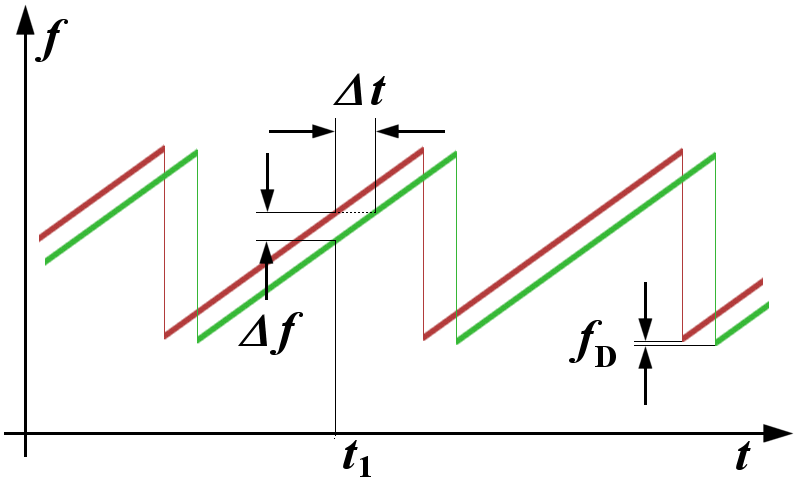
\includegraphics[width=0.75\textwidth]{data/fmcw-principle}
        \caption{FMCW radar operation: a delayed signal is modulated with the original signal and
          the distance to the remote object can be backed out from the phase difference between the
          two signals.}
        \label{fig:fmcw-principle}
\end{figure}

\begin{equation}
        \label{eq:fmcw-principle}
        d = \frac{c t_{\text{ramp}} \Delta f}{2 f_{\text{ramp}}}
\end{equation}

To calculate the frequency difference, we first express it in terms of the round-trip time,
$t_{\text{d}}$:

\begin{equation}
        \Delta f = \frac{t_{\text{d}} f_{\text{ramp}}}{t_{\text{ramp}}}
\end{equation}

The transmitted signal during one ramp is:

\begin{align}
  f(t) &= \sin\left(\omega t\right) \\
       &= \sin\left(2 \pi f(t) t\right) \\
       &= \sin\left(2 \pi t \left( f_0 + t \frac{f_{\text{ramp}}}{t_{\text{ramp}}} \right) \right)
\end{align}

The received signal (which is just a phase shifted version of the transmitted signal) is
$f(t-t_{\text{d}})$. Using the mixer output we can compute the time delay:

\begin{align}
  m &= f(t) f(t-t_{\text{d}}) && \text{$m$ is the mixer output.} \\
    &= \sin(\omega t) \sin(\omega (t-t_{\text{d}})) \\
    &= \cos(\omega t_{\text{d}})/2 && \text{\footnotemark} \\
  t_{\text{d}} &= \frac{\arccos(2m)}{2 \pi \left(f_0 + t \frac{f_{\text{ramp}}}{t_{\text{ramp}}} \right)}
\end{align}
\footnotetext{We've used the identity
  $\sin\theta\sin\phi = \left[\cos(\theta - \phi) - \cos(\theta + \phi)\right]/2$ and the fact that
  the sum term is outside the IF amplifier pass-band and will be filtered out.}

The distance can be computed with Eq.~\ref{eq:fmcw-distance}.

\begin{equation}
        \label{eq:fmcw-distance}
        d = \frac{c \arccos(2m)}{4 \pi \left(f_0 + t \frac{f_{\text{ramp}}}{t_{\text{ramp}}} \right)}
\end{equation}

\section{Angle Calculation}
\label{sec:angle}



\chapter{Circuit Description}
\label{cha:circuit}

\section{Power}
\label{sec:power}
\textit{\hyperlink{schematic.8}{schematic}}

\fixme{I think this section needs information about PSRRs, especially for regulators that feed RF
  circuits.}

\fixme{Another thing that needs clarification is where should the LDO's be placed? Should they be
  located near the loads they serve or the switching converters? My guess would be near the
  converters since that decreases the part of the board that is exposed to the switching noise.}

\subsection{Overview}
\label{sec:power-overview}

A barrel jack is used to feed a 12V input to the board which is then administered to a 10V output
linear regulator and two buck converters that output 5.6V and 3.6V. The buck converters in turn pass
their voltages on to several LDO voltage regulators for input to the various digital ICs on the
board. The benefit of chaining switching converters to linear regulators is greater energy
efficiency and better noise suppression than can be achieved by using either alone. An LED indicates
when power is administered to the board.

\subsection{Barrel Jack / Power Input}
\label{sec:power-input}

A ferrite bead pi filter is placed at the output of the barrel jack connection. The ferrite bead is
rated for $5.1A$, which is more than double the absolute max current draw of the radar. The barrel
connector is a switched jack, but we do not use a battery on this PCB so the 3rd pin is grounded.

\subsection{TPS5420D Buck Converter}
\label{sec:tps5420d}

\subsubsection{Description}
\label{sec:tps5420d-description}

The TPS5420D is an internally-compensated buck converter with a fixed switching frequency of
$500\si{kHz}$, whose block diagram is shown in Figure~\ref{fig:tps5420d-block}. The converter first
compares the divided voltage output with a $1.221V$ reference and uses an error amplifier to amplify
the difference. It then feeds that difference into a PWM comparator along with a sawtooth ramp
waveform. If the PWM comparator outputs a high voltage the switch is turned off, effectively
decreasing the duty cycle. Conversely, a low voltage saturates the transistor and increases the duty
cycle. This has the effect of converging the output voltage to its set point. The TPS5420 has a ramp
time of between $6.6$ and $10 \si{ms}$.

\begin{figure}[h]
        \centering
        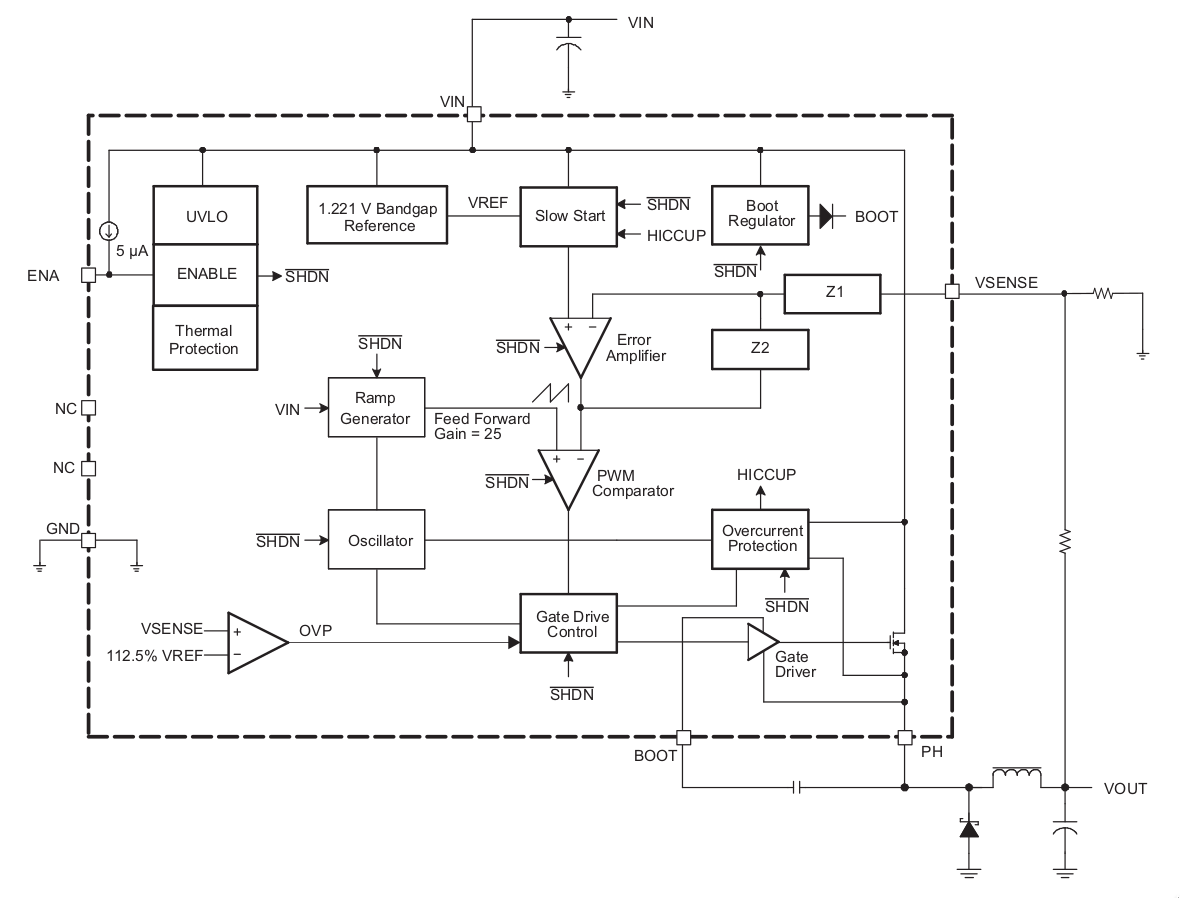
\includegraphics[width=0.9\textwidth]{data/tps5420d-block-diagram}
        \caption{TPS5420D Block Diagram}
        \label{fig:tps5420d-block}
\end{figure}

\subsubsection{Pinout}
\label{sec:tps5420d-pinout}

\fixme{What is the point of BOOT?}
\label{tab:tps5420d-pinout}
\begin{tabularx}{\textwidth}{l l X}
        \caption{TPS5420D pinout.}                                                               \\
        \toprule
        \textbf{\#} & \textbf{Pin} & \textbf{Description}                                        \\
        \midrule
        1           & BOOT         &                                                             \\
        2, 3        & NC           & No connect.                                                 \\
        4           & VSENSE       & Feedback voltage for the regulator. This compares the divided output with a 1.221V
        reference.                                                                               \\
        5           & ENA          & Enable pin. This can be left floating to enable the device. \\
        6           & GND          & Ground.                                                     \\
        7           & VIN          & Input supply voltage.                                       \\
        8           & PH           & Output voltage.                                             \\
        \bottomrule
\end{tabularx}

\subsubsection{Component Selection}
\label{sec:tps5420d-component-selection}

An inductor is chosen such that it satisfies the following 3 requirements:
\begin{enumerate}
\item The inductance is given by Equation~\ref{eq:buck-inductance}.
\item The current rating is at least 2x the maximum load current.
\item The self-resonant frequency is at least 10x the switching frequency.
\end{enumerate}

\begin{equation}
        \label{eq:buck-inductance}
        L_{\text{min}} = \frac{T}{2} \frac{V_{\text{out}}}{I_{\text{out(min)}}} \left(1 -
                \frac{V_{\text{out}}}{V_{\text{in}}}\right)
\end{equation}

The requirements are given in Table~\ref{tab:buck-inductor-reqs}. All of these requirements are
satisfied by the \href{https://www.bourns.com/docs/Product-Datasheets/SRR1210A.pdf}{SRR1210A-330M}
$33\si{\mu H}$ Bourns ferrite bead.

\label{tab:buck-inductor-reqs}
\begin{tabularx}{\textwidth}{c c c c}
        \caption{TPS5420D inductor requirements. I've assumed an input ripple of $300\si{mV}$.} \\
        \toprule
        \textbf{Buck Vout} & \textbf{Lmin}    & \textbf{Current Rating} & \textbf{SRF min}      \\
        \midrule
        \endhead
        $5.6\si{V}$        & $6.5\si{\mu H}$  & $2.21\si{A}$            & $5\si{MHz}$           \\
        $3.6\si{V}$        & $15.1\si{\mu H}$ & $2.50\si{A}$            & $5\si{MHz}$           \\
        \bottomrule
\end{tabularx}

The input, output and boot capacitors were chosen by the \href{https://webench.ti.com}{WEBENCH
  tool}. The flyback diode was chosen to support $2A$ of current.

\subsubsection{Downstream Current Draw}
\label{sec:tps5420d-current}

It is important to know both the maximum and minimum current draw of components whose voltage inputs
are fed by the output of a buck converter. The minimum current sets a lower bound on the inductance
that can be used (see Equation~\ref{eq:buck-inductance}) since the converter must remain in CCM for
proper operation. It is also important to ensure that the buck converter and inductor are rated for
the maximum current draw of downstream devices. Saturating the ferrite-core inductor can cause a
loss in inductance.

\label{tab:buck-5.6-current}
\begin{tabularx}{\textwidth}{l c c X>{\raggedright\arraybackslash}X}
        \caption{The current draw of components downstream from the 5.6V buck converter. When
          minimum current draw is omitted from the datasheet I've assumed 0A.}                                                 \\
        \toprule
        \textbf{MFN}                     & \textbf{I\textsubscript{Q}} & \textbf{I\textsubscript{max}} &
        \textbf{Voltage Inputs}                                                                                                \\
        \midrule
        \hyperlink{sec:adl5802}{ADL5802} & $170\si{mA}$                & $300\si{mA}$                  & 5V                    \\
        \hyperlink{sec:adf4158}{ADF4158} & $312.5\si{\mu A}$           & $5\si{mA}$                    & 5V (VP)               \\
        \hyperlink{sec:se5004l}{SE5004L} & $300\si{mA}$                & $800\si{mA}$                  & 5V (VCC1, VCC2, VCC3) \\
        \midrule
        Total                            & $470\si{mA}$                & $1.105\si{A}$                 & -                     \\
        \bottomrule
\end{tabularx}

\label{tab:buck-3.6-current}
\begin{tabularx}{\textwidth}{l c c X>{\raggedright\arraybackslash}X}
        \caption{Components downstream from the 3.6V buck converter.} \\
        \toprule
        \textbf{MFN} & \textbf{I\textsubscript{Q}} & \textbf{I\textsubscript{max}} & \textbf{Voltage
          Inputs} \\
        \midrule
        \hyperlink{sec:kt2520k}{KT2520K}  & - & $2\si{mA}$ & 1.8V \\
        \hyperlink{sec:nc7s04}{NC7S04} & $1\si{\mu A}$ & $12.5\si{mA}$ & 3.3V \\
        \hyperlink{sec:nb3n551}{NB3N551} & - & $40\si{mA}$ & 3.3V \\
        \midrule
        \hyperlink{sec:xc7a15t-ftg256}{XC7A15T-FTG256} & $97\si{mA}$ & $277\si{mA}$ & 1V (VCCINT,
        VCCBRAM) \\
        XC7A15T-FTG256 & $22\si{mA}$ & $87\si{mA}$ & 1.8V (VCCADC, VCCAUX) \\
        XC7A15T-FTG256 & $1\si{mA}$ & $201\si{mA}$ & 3.3V (VCC0) \\
        \hyperlink{sec:w25q32jv}{W25Q32JV} & $10\si{\mu A}$ & $25\si{mA}$ & 3.3V \\
        \midrule
        \hyperlink{sec:ft2232h}{FT2232H} & $510\si{\mu A}$ & $280\si{mA}$ & 3.3V (VPHY, VPLL, VCORE,
        VCCIO) \\
        \hyperlink{sec:93lc46b}{93LC46B} & - & $2\si{mA}$ & 3.3V \\
        \midrule
        \hyperlink{sec:ltc2292}{LTC2292} & $5\si{mA}$ & $95\si{mA}$ & 3.3V (OVDD), 3V (VDD) \\
        \midrule
        \hyperlink{sec:ada4940-2}{ADA4940-2} & $4.2\si{mA}$ & $5.52\si{mA}$ & 3.3V \\
        \midrule
        \hyperlink{sec:adf4158}{ADF4158} & - & $32\si{mA}$ & 3.3V (AVDD, DVDD) \\
        \midrule
        \hyperlink{sec:hmc431lp4}{HMC431LP4} & $19\si{mA}$ & $27\si{mA}$ & 3V \\
        \midrule
        \hyperlink{sec:trf37a73}{TRF37A73} & $250\si{\mu A}$ & $130\si{mA}$ & 3V \\
        \hyperlink{sec:sky65404}{SKY65404} & $20\si{mA}$ & $36\si{mA}$ & 3V (VENABLE, VCC) \\
        \midrule
        Total & $169\si{mA}$ & $1.252\si{A}$ & - \\
        \bottomrule
\end{tabularx}

\subsubsection{PCB Layout}
\label{sec:tps5420d-pcb}

The datasheet provides a suggested PCB layout, shown in Figure~\ref{fig:tps5420d-pcb}.

\begin{figure}[h]
        \centering
        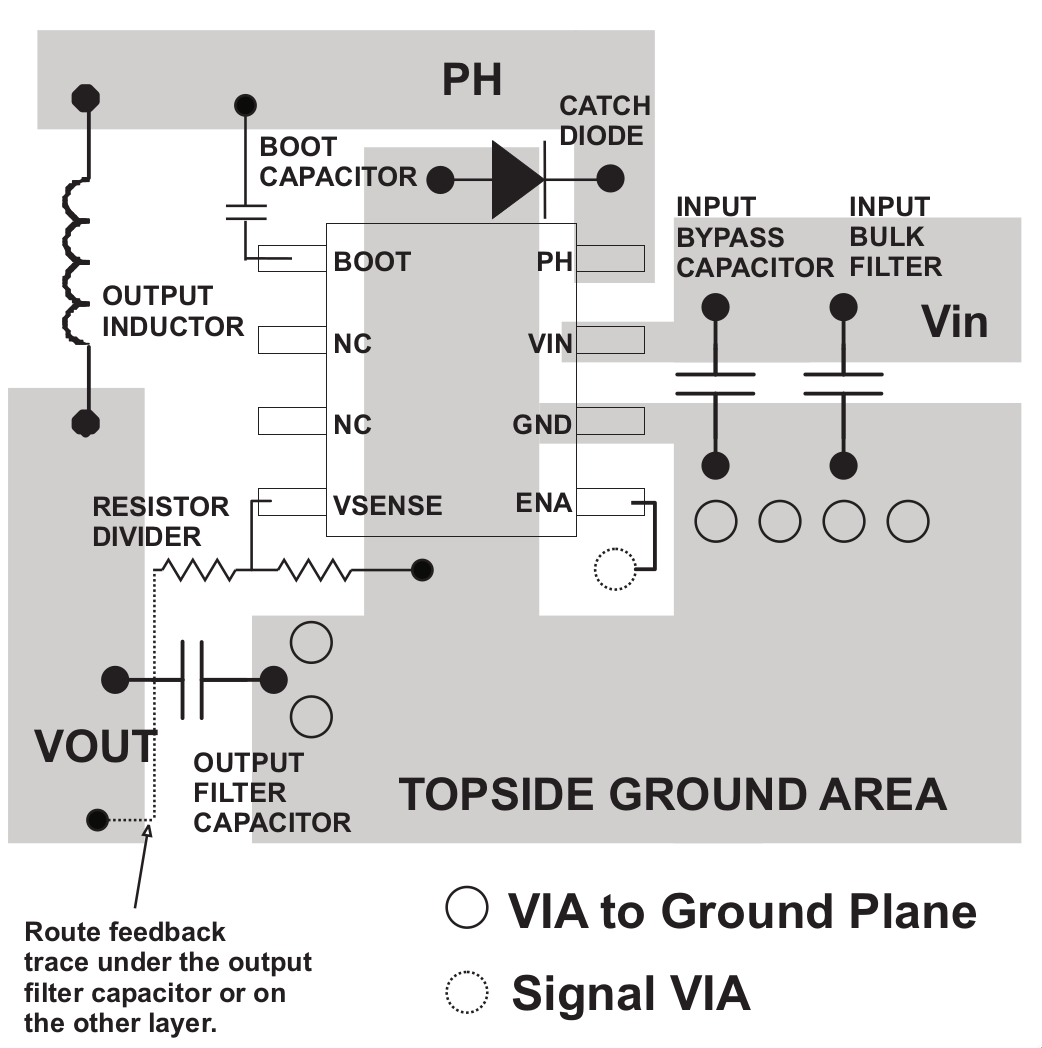
\includegraphics[width=0.75\textwidth]{data/tps5420d-pcb.png}
        \caption{TPS5420D suggested PCB layout.}
        \label{fig:tps5420d-pcb}
\end{figure}

\subsection{TPS560200 Buck Converter}
\label{sec:tps560200}

\subsubsection{Description}
\label{sec:tps560200-description}

The TPS560200 is an internally-compensated buck converter with a switching frequency of
$600 \si{kHz}$ and a fixed ramp time of $2 \si{ms}$. It is needed, rather then a linear regulator
chained to a TPS5420D, because the FPGA requires its $1 \si{V}$ power supply first.

\subsubsection{Pinout}
\label{sec:tps560200-pinout}

\label{tab:tps560200-pinout}
\begin{tabularx}{\textwidth}{l l X}
        \caption{TPS50600 pinout.}                                                 \\
        \toprule
        \# & Pin    & Description                                                  \\
        \midrule
        1  & EN     & Enable pin. Can be floated to unconditionally enable device. \\
        2  & GND    & Ground.                                                      \\
        3  & PH     & Output voltage.                                              \\
        4  & VIN    & Input voltage.                                               \\
        5  & VSENSE & Feedback, compared to a $0.8 \si{V}$ reference.              \\
        \bottomrule
\end{tabularx}

\subsubsection{Component Selection}
\label{sec:tps560200-component-selection}

The voltage divider resistors, filter capacitors and input capacitors are specified by the
datasheet. The output voltage ripple must be sufficiently small that it falls within the required
voltage range of the FPGA's V\textsubscript{CCINT} input. Specifically, it must be less than
$100 \si{mV}$. Texas Instruments provides\footnote{\url{www.ti.com/lit/an/slva630a/slva630a.pdf}} an
equation for the voltage ripple of a buck converter, given a small capacitor resistance. I'm further
assuming an ESR of 0 since I'm using ceramic capacitors at the output and the current draw is fairly
low. The equation is provided in Equation~\ref{eq:tps560200-ripple-voltage}. The ripple current for
a buck converter is given in Equation~\ref{eq:tps560200-ripple-current}. Finally, the remaining
inductor requirements are specified in Table~\ref{tab:tps560200-inductor-reqs}. All of these
requirements are satisfied by a $10 \si{\mu H}$ inductor, which is used in the datasheet. However,
this puts the inductor a bit close to DCM and since I have extra $33 \si{\mu H}$ inductors on hand
I'd rather be safe and use one of those.

\begin{equation}
        \label{eq:tps560200-ripple-voltage}
        V_{\text{p2p}} = \frac{I_{\text{p2p}}}{8 C F_{\text{SW}}}
\end{equation}

\begin{equation}
        \label{eq:tps560200-ripple-current}
        I_{\text{p2p}} = V_{\text{out}} \frac{1 - D}{L F_{\text{SW}}}
\end{equation}

\label{tab:tps560200-inductor-reqs}
\begin{tabularx}{\textwidth}{c c c c}
        \caption{TPS560200 inductor requirements.}                                            \\
        \toprule
        V\textsubscript{out} & L\textsubscript{min} & Current Rating & SRF\textsubscript{min} \\
        \midrule
        $1 \si{V}$           & $7.9 \si{\mu H}$     & $554 \si{mA}$  & $6 \si{MHz}$           \\
        \bottomrule
\end{tabularx}

\subsubsection{Downstream Current Draw}
\label{sec:tps560200-current}

\label{tab:tps560200-current}
\begin{tabularx}{\textwidth}{l c c X}
        \caption{Components downstream from the TPS560200 buck converter.} \\
        \toprule
        MFN & I\textsubscript{Q} & I\textsubscript{max} & Voltage Inputs \\
        \midrule
        \hyperlink{sec:xc7a15t-ftg256}{XC7A15T-FTG256} & $97\si{mA}$ & $277\si{mA}$ & 1V (VCCINT,
        VCCBRAM) \\
        \bottomrule
\end{tabularx}

\subsubsection{PCB Layout Guidelines}
\label{sec:tps560200-pcb}

The datasheet provides a recommended layout, shown in Figure~\ref{fig:tps560200-pcb}.

\begin{figure}[h]
        \centering
        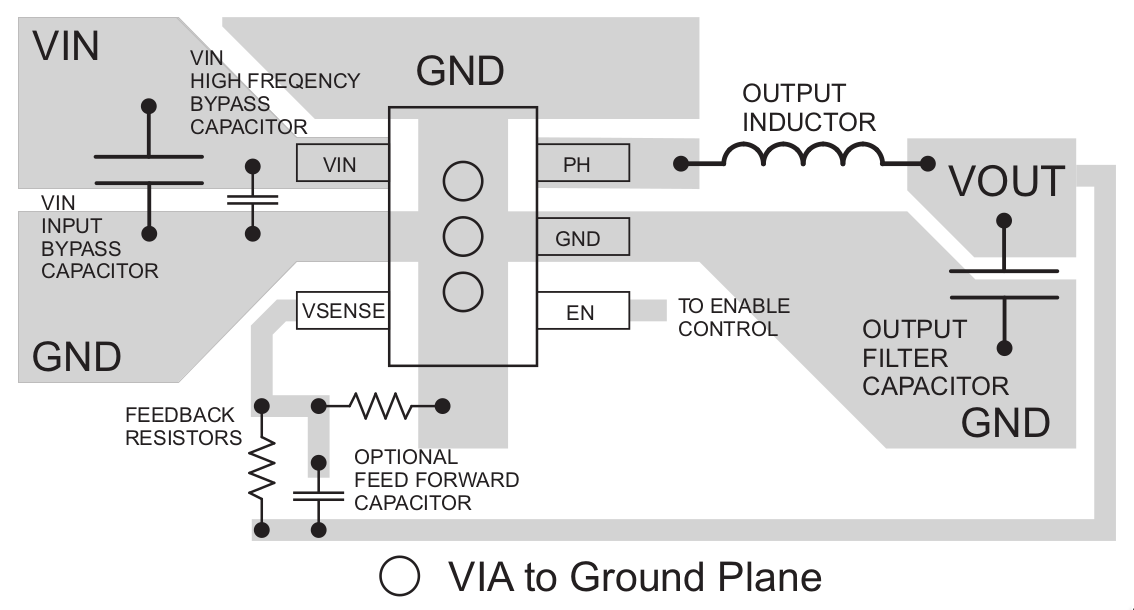
\includegraphics[width=0.75\textwidth]{data/tps560200-pcb}
        \caption{TPS560200 recommended PCB layout.}
        \label{fig:tps560200-pcb}
\end{figure}

\subsection{LP2985A-10DBVR Linear Regulator}
\label{sec:lp2985a-10dbvr}

\subsubsection{Description}
\label{sec:lp2985a-10dbvr-description}

The LP2985A is a low-dropout fixed-output regulator with a max output current of $150\si{mA}$. It's
functional block diagram is shown in Figure~\ref{fig:lp2985a-block-diagram}. It uses an op-amp to
compare the voltage-divided output with a $1.23\si{V}$ reference. It then turns a PNP transistor
on/off depending on the output voltage level relative to its $10\si{V}$ target.

\begin{figure}[h]
        \centering
        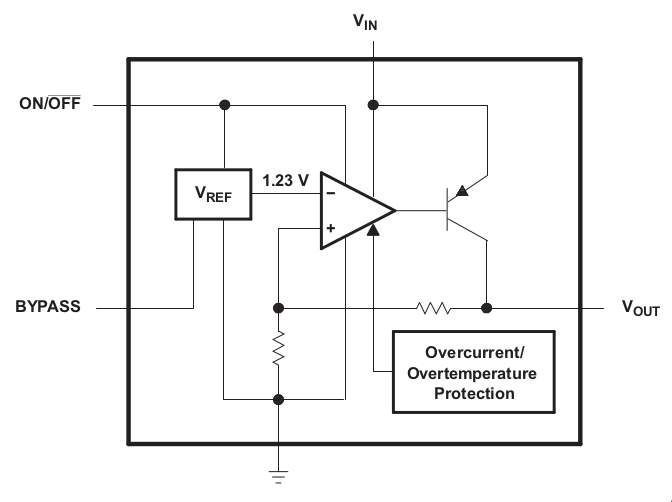
\includegraphics[width=0.5\textwidth]{data/lp2985a-block-diagram}
        \caption{The LP2985A-10DBVR LDO regulator block diagram.}
        \label{fig:lp2985a-block-diagram}
\end{figure}

\subsubsection{Pinout}
\label{sec:lp2985a-10dbvr-pinout}

\label{tab:lp2985a-10dbvr-pinout}
\begin{tabularx}{\textwidth}{l l X}
        \caption{LP2985A's pin descriptions.}							\\
        \toprule
        \textbf{\#}	&	\textbf{Pin}		&	\textbf{Description}		\\
        \midrule
        1		&	VIN			&	Voltage supply.			\\
        2		&	GND			&	Ground.				\\
        3		&	ON/\textoverline{OFF}	&	Active-low shutdown pin. It is tied
	to VIN since the device should be unconditionally enabled. \\
        4		&	BYPASS			&	Connected to a $10\si{nF}$ capacitor
	to ground to decrease output voltage noise. \\
        5		&	VOUT			&	Regulated, voltage output.	\\
        \bottomrule
\end{tabularx}

\subsubsection{Component Selection}
\label{sec:lp2985a-10dbvr-component-selection}

The input capacitor should be at least $1\si{\mu F}$ and the output capacitor should be at least
$2.2\si{\mu F}$, but higher values are better at the output. I'm using $10\si{\mu F}$.

\subsubsection{Downstream Current Draw}
\label{sec:lp2985a-10dbvr-current}

\label{tab:lp2985a-10dbvr-current}
\begin{tabularx}{\textwidth}{l c c X}
        \caption{Downstream current draw for the 10V linear regulator.} \\
        \toprule
        MFN & I\textsubscript{Q} & I\textsubscript{max} & Voltage Inputs \\
        \midrule
        \hyperlink{sec:tlv172dck}{TLV172DCK} & $1.6\si{mA}$ & $75\si{mA}$ & 10V \\
        \bottomrule
\end{tabularx}

\subsubsection{PCB Layout}
\label{sec:lp2985a-10dbvr-pcb}

The input and output capacitors should be placed within $1\si{cm}$ of the input and output pins and
have a low-impedance path to ground.

\subsection{TPS7A91 LDO Voltage Regulator}
\label{sec:tps7a91}

\subsubsection{Description}
\label{sec:tps7a91-description}

The TPS7A91 is a low-noise, low-dropout and adjustable voltage regulator. It has an RMS output noise
of $4.7 \si{\mu V}$. The regulator works by comparing the feedback voltage, at the inverting input
of an error amplifier, with a $0.8 \si{V}$ reference voltage at the non-inverting input. The output
of the error amplifier is connected to the gate of an n-channel MOSFET whose drain is attached to
the input voltage and whose source is attached to the output voltage. This negative feedback creates
a stable equilibrium when the output voltage is at its set-point. The functional block diagram is
shown in Figure~\ref{fig:tps7a91-block-diagram}.

The power-good function of one regulator is used to ensure that the $1.8 \si{V}$ supply arrives at
the FPGA before the $3.3 \si{V}$ supply. The circuit uses an open-drain output with a pull-up
resistor. If the output voltage goes below some threshold, the MOSFET will saturate and the PG line
will be brought low. Otherwise, it will be pulled high.

\begin{figure}[h]
        \centering
        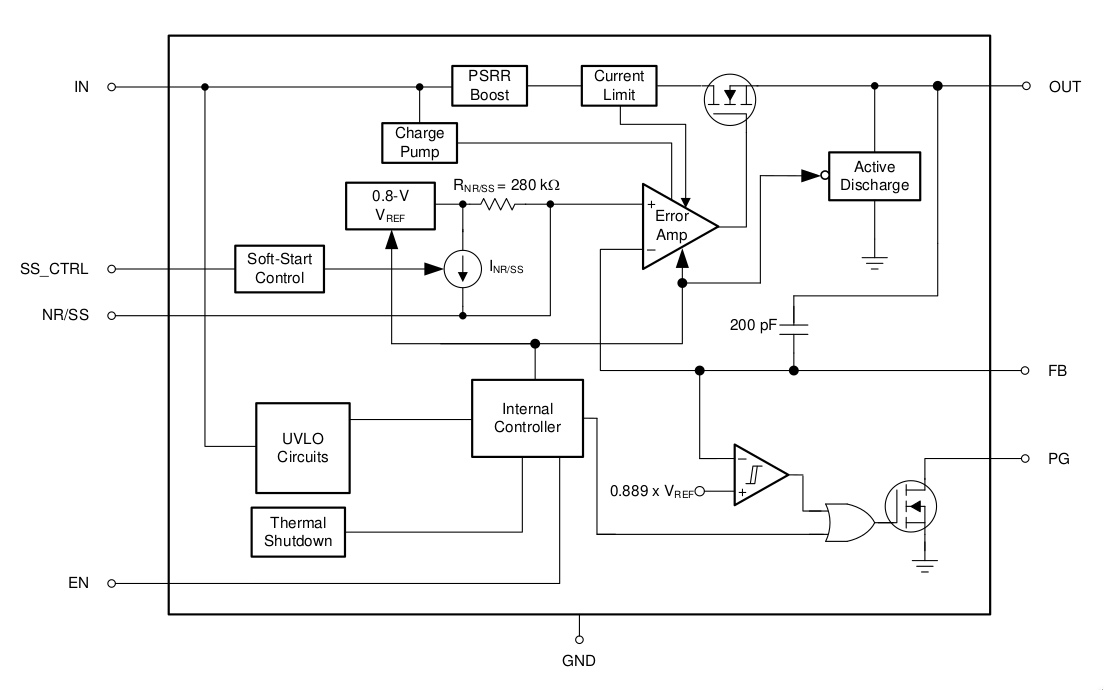
\includegraphics[width=0.75\textwidth]{data/tps7a91-block-diagram}
        \caption{TP7A91 block diagram.}
        \label{fig:tps7a91-block-diagram}
\end{figure}

\subsubsection{Pinout}
\label{sec:tps7a91-pinout}

\label{sec:tps7a91-pinout}
\begin{tabularx}{\textwidth}{l l X}
        \caption{TPS7A91 pinout.} \\
        \toprule
        \# & Pin & Description \\
        \midrule
        1, 2 & OUT & Regulated output voltage. A $10 \si{\mu F}$ or greater
        capacitor should be
        connected between this pin and ground. \\
        3 & FB & Feedback pin. The divided output voltage is compared against a $0.8 \si{V}$
        reference. \\
        4 & GND & Ground. \\
        5 & PG & A power good indicator that can signal to downstream devices when voltage is within
        some range of the desired level. The design doesn't use this and so the pin has been left
        floating. \\
        6 & SS\_CTRL & Soft-start control pin. Tying this pin to the input voltage increases the
        soft-start charging current to $100 \si{\mu A}$, which reduces the startup time. This pin
        could have also been tied to ground if a slower startup time was desired. \\
        7 & EN & Enable. Tying this to the input voltage unconditionally enables this device. \\
        8 & NR/SS & Noise-reduction pin. A capacitor can be placed between this pin and ground
        to reduce output noise. This effectively acts like an RC filter. A capacitance between $10
        \si{nF}$ and $1 \si{\mu F}$ is recommended. I've used $100 \si{nF}$. This pin also limits
        inrush current. \\
        9, 10 & IN & Input voltage pin. A bypass capacitor of $10 \si{\mu F}$ or more is
        required. \\
        \bottomrule
\end{tabularx}

\subsubsection{Component Selection}
\label{sec:tps7a91-component-selection}

MLCC capacitors are recommended for input and output bypassing due to their low ESR, with
preferences given to X5R and X7R types. Additionally, they should be derated by at least 50\%. The
recommended capacitance is $10 \si{\mu F}$ or greater at the input and output. I've used
$10 \si{\mu F}$ at the input and the same at the output, with the option for another capacitor at
the output if needed. The $10 \si{nF}$ feed-forward capacitor between FB and OUT is recommended by
the datasheet to improve noise and PSRR performance. The voltage divider resistors are specifically
mentioned in the datasheet to get the appropriate output values.

\subsubsection{PCB Layout}
\label{sec:tps7a91-pcb}

The recommended PCB layout is shown in Figure~\ref{fig:tps7a91-pcb}.

\begin{figure}[h]
        \centering
        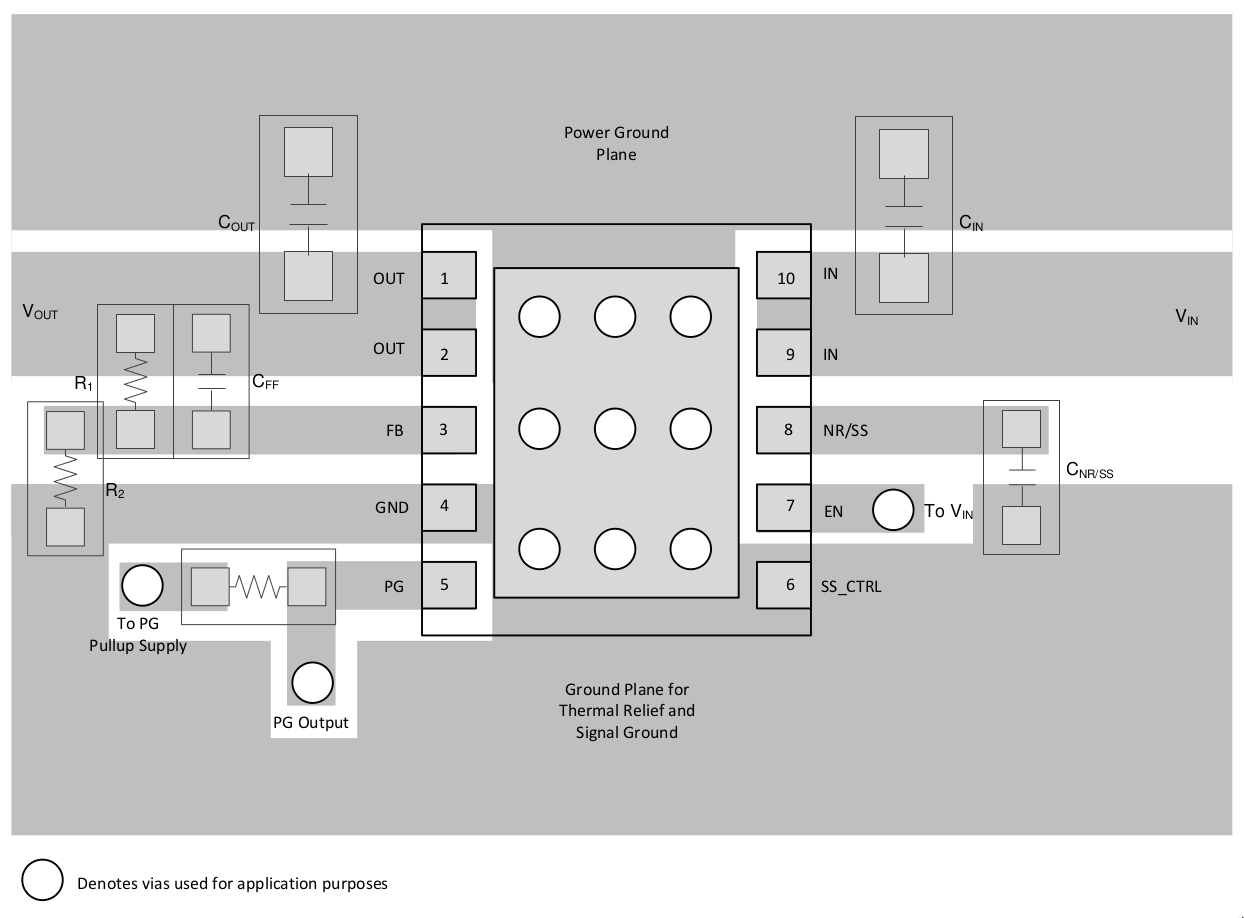
\includegraphics[width=0.75\textwidth]{data/tps7a91-pcb}
        \caption{TPS7A91 recommended PCB layout.}
        \label{fig:tps7a91-pcb}
\end{figure}

\subsection{TPS7A7001DDA LDO Regulator}
\label{sec:tps7a7001dda}

\subsubsection{Description}
\label{sec:tps7a7001dda-description}

The TPS7A7001DDA supports low dropouts up to $2 \si{A}$, which is important since it must
accommodate a maximum current draw of $1.1 \si{A}$ (see Table~\ref{tab:buck-5.6-current}).

\subsubsection{Pinout}
\label{sec:tps7a7001dda-pinout}

\label{tab:tps7a7001dda-pinout}
\begin{tabularx}{\textwidth}{l l X}
        \caption{TPS7A7001DDA pinout.}                                \\
        \toprule
        \#      & Pin & Description                                   \\
        \midrule
        1, 4, 5 & NC  & No connect.                                   \\
        2       & EN  & Enable input. Connected to IN since unused.   \\
        3       & IN  & Input voltage.                                \\
        6       & OUT & Regulated voltage output.                     \\
        7       & FB  & Feedback, compared to $0.5 \si{V}$ reference. \\
        8       & GND & Ground.                                       \\
        9       & EP  & Exposed pad. Tied to ground.                  \\
        \bottomrule
\end{tabularx}

\subsubsection{Component Selection}
\label{sec:tps7a7001dda-component-selection}

An input capacitor of $1 - 10 \si{\mu F}$ and with low ESR is recommended. The output capacitor
should be ceramic and can be anywhere from $4.7 - 47 \si{\mu F}$. I've chosen $10 \si{\mu F}$ with
the option for an additional capacitor if needed. The voltage divider resistors are specifically
recommended by the datasheet.

\subsubsection{PCB Layout}
\label{sec:tps7a7001dda-pcb}

The recommended PCB layout is provided in~\ref{fig:tps7a7001dda-pcb}.

\begin{figure}[h]
        \centering
        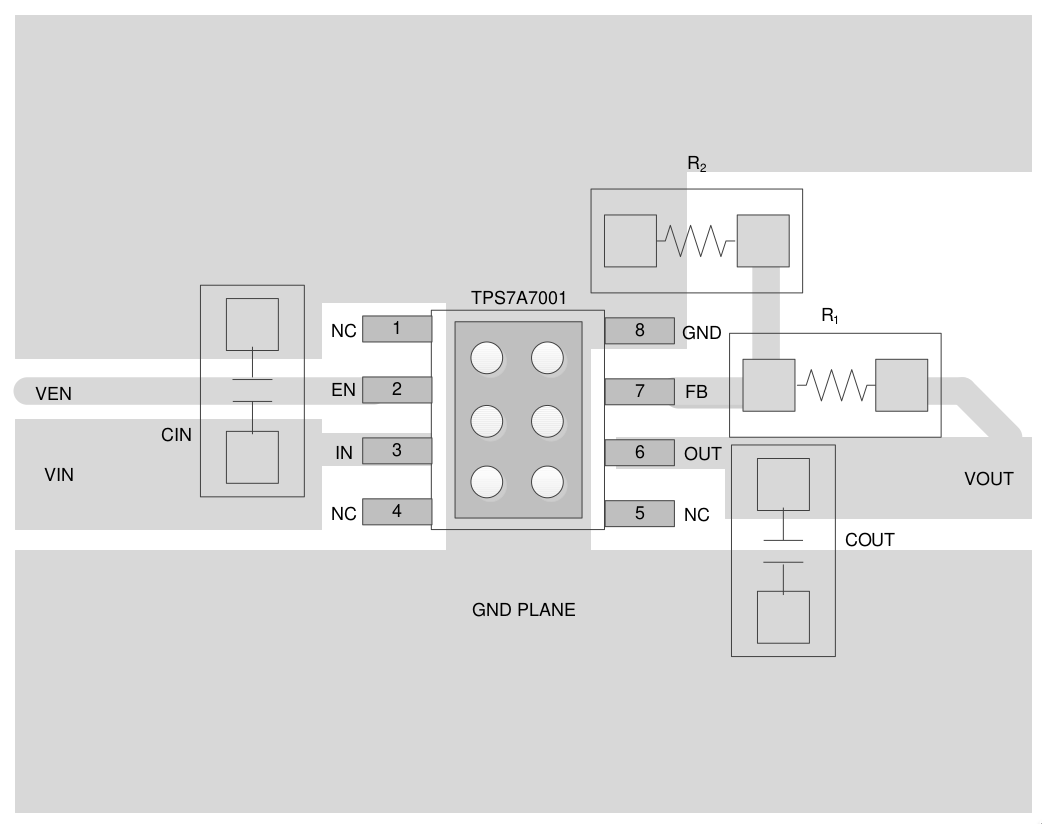
\includegraphics[width=0.75\textwidth]{data/tps7a7001dda-pcb}
        \caption{TPS7A7001DDA recommended PCB layout.}
        \label{fig:tps7a7001dda-pcb}
\end{figure}

\subsection{LP5907MFX-3.0}
\label{sec:mic5301-3.3}

\subsubsection{Description}
\label{sec:mic5301-3.3-description}

The LP5907MFX-3.0 is a low-noise and dropout voltage regulator used to power the VCO and
reception-side amplifiers. It has a current rating of $250 \si{mA}$ which is more than the maximum
current load of the downstream components.

\subsubsection{Pinout}
\label{sec:lp5907mfx-3.0-pinout}

\label{tab:lp5907mfx-3.0-pinout}
\begin{tabularx}{\textwidth}{l l X}
        \caption{LP5907MFX-3.0 pinout.}                                      \\
        \toprule
        \# & Pin & Description                                               \\
        \midrule
	1  & IN  & Voltage input.                                            \\
	2  & GND & Ground.                                                   \\
	3  & EN  & Enable. Tied to IN to keep the device unconditionally on. \\
	4  & NC  & No connect.                                               \\
	5  & OUT & $1.8 \si{V}$ output.                                      \\
        \bottomrule
\end{tabularx}

\subsubsection{Component Selection}
\label{sec:lp5907mfx-3.0-component-selection}

The input and output capacitors should be $1 - 10 \si{\mu F}$, with the input capacitor at least as
large as the output capacitor. I've used $10 \si{\mu F}$ capacitors in this design.

\subsubsection{PCB Layout}
\label{sec:lp5907-3.0-pcb}

The recommended PCB layout is shown in Figure~\ref{fig:lp5907mfx-3.0-pcb}.

\begin{figure}[h]
	\centering
	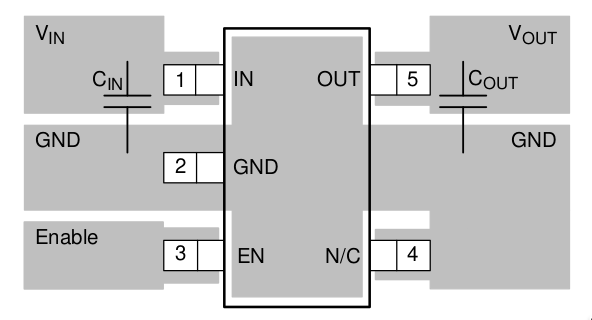
\includegraphics[width=0.5\textwidth]{data/lp5907mfx-3-pcb}
	\caption{LP5907MFX-3.0 recommended PCB layout.}
	\label{fig:lp5907mfx-3.0-pcb}
\end{figure}

%%% Local Variables:
%%% mode: latex
%%% TeX-master: "fmcw-radar"
%%% End:

\section{Top}
\label{sec:top}
\textit{\hyperlink{schematic.1}{schematic}}

\subsection{Overview}
\label{sec:top-overview}

The top-level schematic has two purposes: it instantiates the various submodules in the design and
generates a $40 \si{MHz}$ clock signal that is distributed to the
\hyperref[sec:xc7a15t-ftg256]{FPGA}, \hyperref[sec:ltc2292]{ADC} and
\hyperref[sec:adf4158]{frequency synthesizer}.

The \hyperref[sec:kt2520k]{crystal oscillator} has its own $1.8 \si{V}$ power supply and the
\hyperref[sec:nc7svu04]{inverter} and \hyperref[sec:nb3n551]{clock buffer} share their own
$3.3 \si{V}$ power supply. The LDO used is a very low noise \hyperref[sec:lp5907]{LP5907}. However,
the PSRR of the LDO at the switching frequency of the \hyperref[sec:tps5420d]{buck converter that
  feeds it} is greatly diminished from it's lower frequency value ($80 \si{dB}$ at $1 \si{kHz}$ and
only about $40 \si{dB}$ at $500 \si{kHz}$). So, ferrite bead pi filters are used at the LDO outputs
to provide further noise suppression for higher frequencies. They also prevent noise generated by
the clocks from reentering the power supply and affecting other devices.

\subsection{KT2520K 40MHz TXCO}
\label{sec:kt2520k}

\subsubsection{Description}
\label{sec:kt2520k-description}

The KT2520K crystal oscillator outputs a $40 \si{MHz}$ clipped sine wave. It requires a DC-blocking
capacitor $\geq 1 \si{nF}$ at the output since one is not included internally. I've used $100
\si{nF}$ which is recommended by the \hyperref[sec:ltc2292]{ADC} datasheet.

\subsection{NC7SVU04 Inverter}
\label{sec:nc7svu04}

\subsubsection{Description}
\label{sec:nc7svu04-description}

The NC7SVU04 is a high-speed logic inverter used to convert its clipped sine-wave input into a
square wave output. It has a typical propagation delay of $1.5 \si{ns}$.

\subsubsection{Component Selection}
\label{sec:nc7svu04-component-selection}

The inverter configuration is specified by the \hyperref[sec:ltc2292]{ADC} datasheet. The voltage
divider sets the DC bias point at $V_{\text{CC}}/2$, which in turn sets the duty cycle to 50\%. The
coupling capacitor is required because the crystal oscillator has low operational voltage and it
allows the divider to set the DC bias point.

\subsubsection{PCB Layout}
\label{sec:nc7svu04-pcb}

The oscillator, inverter and buffer should be placed adjacent to the ADC, which is very susceptible
to noise from clock jitter.

\subsection{NB3N551 1:4 Clock Buffer}
\label{sec:nb3n551}

\subsubsection{Description}
\label{sec:nb3n551-description}

The NB3N551 clock buffer duplicates the square wave input clock signal into 3 identical clock
outputs that are fed to the FPGA, ADC and frequency synthesizer.

\subsubsection{Component Selection}
\label{sec:nb3n551-component-selection}

A $33 \si{\Omega}$ source terminating resistor is used for the \hyperref[sec:xc7a15t-ftg256]{FPGA}
and \hyperref[sec:adf4158]{frequency synthesizer} clock lines because the traces leading to their
clock pins are longer than 1 inch. This prevents noise from the FPGA and frequency synthesizer from
affecting the clock fan-out. The source terminating resistor is not used for the ADC line because it
is assumed that the fan-out buffer is immediately adjacent to the ADC\@. However, if the clock is
placed farther away, the $33 \si{\Omega}$ must be used on this line as well.

%%% Local Variables:
%%% mode: latex
%%% TeX-master: "fmcw-radar"
%%% End:

\section{FPGA}
\label{sec:fpga}

\subsection{Overview}
\label{sec:fpga-overview}

The FPGA has two main roles. It performs digital signal processing on data sent from the ADC and
relays the processed data back to a host computer via an \hyperlink{sec:ft2232h}{FT2232H} which acts
as a FIFO-USB interface. Secondly, the FPGA is used to configure other components on the board. In
order to program the FPGA, we use a host computer with a JTAG interface via the FT2232H.

The FPGA stores and loads its configuration from an SPI flash memory device,
\hyperlink{sec:w25q32jv}{W25Q32JV}.

\subsection{XC7A15T-FTG256 Xilinx FPGA}
\label{sec:xc7a15t-ftg256}

\subsubsection{Documents}
\label{sec:xc7a15t-ftg256-documents}

\label{tab:xc7a15t-ftg256-documents}
\begin{tabularx}{\textwidth}{l X>{\raggedright\arraybackslash}X}
        \caption{Important documents.} \\
        \toprule
        \textbf{URL} & \textbf{Description} \\
        \midrule
        \endhead

        \href{https://www.xilinx.com/products/silicon-devices/fpga/artix-7.html?resultsTablePreSelect=documenttype:Data\%20Sheets#documentation}{Artix-7
          FPGA family} & The main page that contains a collection of documents about the 7 series
        devices. \\
        \href{https://www.xilinx.com/support/documentation/user_guides/ug475_7Series_Pkg_Pinout.pdf}{Package
          / Pinout} & The various packages that the device comes in, along with the associated pin
        definitions. \\
        \href{https://www.xilinx.com/support/documentation/data_sheets/ds180_7Series_Overview.pdf}{Overview}
        & Contains
        general device capability information, such as number of logic cells, DSP blocks, etc. \\
        \href{https://www.xilinx.com/support/documentation/user_guides/ug483_7Series_PCB.pdf}{PCB
          Design Guide} &
        Contains information about bypassing and other design considerations. \\
        \href{https://www.xilinx.com/support/documentation/user_guides/ug480_7Series_XADC.pdf}{XADC}
        & Contains
        information about the FPGA's internal ADC. \\
        \href{https://www.xilinx.com/support/documentation/user_guides/ug470_7Series_Config.pdf}{Configuration
          Guide} &
        Describes how to configure the FPGA with a bitstream. \\

        \bottomrule
\end{tabularx}

\subsubsection{Bypassing}
\label{sec:xc7a15t-ftg256-bypassing}

The PCB Design Guide above specifies fairly stringent requirements for bypassing and should be adhered to.

\subsubsection{Pinout}
\label{sec:xc7a15t-ftg256-pinout}

The FPGA pins follow a logical syntax: they can be of the form IO\_LXXY\_ZZZ\_\#, IO\_XX\_ZZZ\_\#,
or a specific name. If they have a specific name, they have a dedicated function described starting
on page 26 of the package-pinout document. If they have the general form IO\_LXXY\_ZZZ\_\# or
IO\_XX\_ZZZ\_\#, they can be used for several different dedicated functions, or as general purpose
IO pins. L indicates that the pin can be used as a differential pair (differential signaling), where
Y=P or N depending on whether the pin is the positive or negative side of the differential pair. XX
gives a unique number identifier that can be used to associate the two different pins forming a
differential pair. ZZZ represents one or more functions that the pin can be used for in addition to
general purpose IO. \# indicates the bank number, which separate the pins into one of several
different regions. The package used in this design is FTG256C, which contains banks 0, 14, 15, 34
and 35. Bank 0 contains the dedicated configuration pins. Each bank has 4 pairs of clock capable
inputs for differential or single ended clocks (there are no global clock pins).


\label{tab:fpga-pins}
\begin{tabularx}{\textwidth}{c X>{\raggedright\arraybackslash}X}
        \caption{All FPGA pin connections in alphabetical order.} \\
        \toprule
        \textbf{PIN} & \textbf{DESCRIPTION} \\
        \midrule
        \endhead

        A01 & GND. \\
        A02 & Connected to an external 1x1 pin header that is currently unused by FPGA logic. \\
        A03 & Connected to external 2x4 pin header that is currently unused by FPGA logic. \\
        A04 & Connected to same pin header as A03. Also unused. \\
        A05 & Same. \\
        A06 & One of the voltage supplies for bank 35. It uses 3.3V as with all the other voltage supplies
        to the main banks of the FPGA. \\
        A07 & Connected to same pin header as A03. Unused. \\
        A08 & A different 2x4 pin header. Unused. \\
        A09 & Connected to the same pin header as A08. Unused. \\
        A10 & Floating. \\
        A11 & GND. \\
        A12 & Connected as an output to the FT2232H USB-JTAG converter. Pulling this low allows the
        FT2232H device to output data to the FPGA through the ADBUS pins. Driving it high sets the ADBUS
        pins as inputs. Remember, the ADBUS pins serve as the bidirectional translation between JTAG data
        and USB data. \\
        A13 & SIWU (channel A). This pin is output to the FT2232H device and can be used to optimize USB
        data transfers (more info in the FT2232H datasheet). It is not currently used by the FPGA
        logic. \\
        A14 & Write output pin to the FT2232H device. When this is driven low, the FPGA writes data to the
        FT2232H. When it's driven high, the FPGA can perform a read from the FT2232H. \\
        A15 & Inputs a 60MHz clock signal that originated at the FT2232H. This clock is used to
        synchronize all data transfers between the FPGA and the FT2232H. \\
        A16 & A 3.3V input to bank 15. \\

        \midrule

        B01 & ADC\_SHDN1. One of two ADC\_SHDN outputs that, together with OEA (B02), controls the
        shutdown mode selection of the ADC. It is used by the digital FPGA logic. When both SHDN and OE
        are grounded, the ADC performs normally. When they are both pulled high, the ADC goes into sleep
        mode. There are two other states but they are not used by the FPGA logic. \\
        B02 & ADC\_OE1. See pin B01. This is used for channel A. \\
        B03 & 3.3V input for bank 35. \\
        B04 & Floating. \\
        B05 & Connected to the same 2x4 pin header as A03. Unused. \\
        B06 & Floating. \\
        B07 & Connected to the same 2x4 pin header as A03. Unused. \\
        B08 & GND. \\
        B09 & Connected to the same pin header as A08. Unused. \\
        B10 & Connected to the same pin header as A08. Unused. \\
        B11 & Floating. \\
        B12 & Floating. \\
        B13 & 3.3V input for bank 15. \\
        B14 & RD\#. A read active-low output pin to the FT2232H device. When this is driven low, the FPGA
        reads data from the FT2232H. \\
        B15 & TXE\#. An active-low input from the FT2232H. FT2232H drives this pin low to signal sending
        data to the FPGA (i.e. a read for the FPGA). \\
        B16 & RXF\#. An active-low input from the FT2232H. FT2232H drives this pin low to signal that it
        should read data. To the FPGA, this signals that it should write data. \\

        \midrule

        C01 & Floating. \\
        C02 & OF1. An input from the ADC. It is pulled high when an overflow or underflow occurs at
        channel A. It is currently unused by the FPGA logic. \\
        C03 & Floating. \\
        C04 & Floating. \\
        C05 & GND. \\
        C06 & Floating. \\
        C07 & Floating. \\
        C08 & Floating. \\
        C09 & Floating. \\
        C10 & 3.3V input to bank 15. \\
        C11 & Connected to the same pin header as A08. Unused. \\
        C12 & Connected to the same pin header as A08. Unused. \\
        C13 & Floating. \\
        C14 & Floating. \\
        C15 & GND. \\
        C16 & FT\_SUSPEND. An active-low input to the FPGA. FT223H drives this low when the USB is in
        suspend mode. It is currently unused by the FPGA logic. \\

        \midrule
        D01 & LED. Connects to an LED that is used by the FPGA to signal data processing. \\
        D02 & GND. \\
        D03 & Floating. \\
        D04 & Floating. \\
        D05 & Floating. \\
        D06 & Floating. \\
        D07 & 3.3V input to bank 35. \\
        D08 & Floating. \\
        D09 & Floating. \\
        D10 & Floating. \\
        D11 & Floating. \\
        D12 & GND. \\
        D13 & Floating. \\
        D14 & Floating. \\
        D15 & FT\_D7. Bidirectional pin 7/7 of ADBUS, used to transmit data between the FPGA andFT2232H. \\
        D16 & FT\_D6. Bidirectional pin 6/7 of ADBUS, used to transmit data between the FPGA andFT2232H. \\

        \midrule

        E01 & D10. Input pin 10/11 of the ADC's channel A digital outputs. It is used to transmit data
        from the ADC to FPGA. \\
        E02 & D11. Input pin 11/11 of the ADC's channel A digital outputs. It is used to transmit data
        from the ADC to FPGA. \\
        E03 & Floating. \\
        E04 & 3.3V input to bank 35. \\
        E05 & Floating. \\
        E06 & Floating. \\
        E07 & CFGPVS\_0. A dedicated pin that is part of the configuration logic of the FPGA. It is used
        to specify the voltage level used for all banks. Since we use 3.3V, we connect this pin to the
        same 3.3V voltage level. \\
        E08 & CCLK\_0. An output pin exported from the FPGA to the flash memory device, W25Q32JV, to drive
        its operation and coordinate writes and reads to and from the device. \\
        E09 & GND. \\
        E10 & VCCBRAM. One of the two power supply pins to the FPGA's internal RAM. It requires 1.0V. \\
        E11 & Floating. \\
        E12 & Floating. \\
        E13 & Floating. \\
        E14 & 3.3V power supply to bank 15. \\
        E15 & FT\_D5. Bidirectional pin 5/7 of ADBUS, used to transmit data between the FPGA and
        FT2232H. \\
        E16 & FT\_D4. Bidirectional pin 4/7 of ADBUS, used to transmit data between the FPGA and
        FT2232H. \\

        \midrule

        F01 & VCC0\_35. 3.3V power supply to bank 35. \\
        F02 & D9. Input pin 9/11 of the ADC's channel A digital outputs. It is used to transmit data from
        the ADC to FPGA. \\
        F03 & Floating. \\
        F04 & Floating. \\
        F05 & Floating. \\
        F06 & GND. \\
        F07 & VCCINT. 1.0V power supply for the internal core logic of the FPGA. \\
        F08 & VCCBATT\_0. Can be used for memory backup. We do not use it so we tie it to GND. \\
        F09 & VCCINT. 1.0V power supply for the internal core logic of the FPGA. \\
        F10 & GND. \\
        F11 & VCCBRAM. One of the two power supply pins to the FPGA's internal RAM. It requires 1.0V. \\
        F12 & Floating. \\
        F13 & Floating. \\
        F14 & FT\_D3. Bidirectional pin 3/7 of ADBUS, used to transmit data between the FPGA and
        FT2232H. \\
        F15 & FT\_D0. Bidirectional pin 0/7 of ADBUS, used to transmit data between the FPGA and
        FT2232H. \\
        F16 & GND. \\

        \midrule

        G01 & D10. Input pin 10/11 of the ADC's channel A digital outputs. It is used to transmit data
        from the ADC to FPGA. \\
        G02 & D7. Input pin 7/11 of the ADC's channel A digital outputs. It is used to transmit data from
        the ADC to FPGA. \\
        G03 & GND. \\
        G04 & Floating. \\
        G05 & Floating. \\
        G06 & VCCINT. 1.0V power supply for the internal core logic of the FPGA. \\
        G07 & GNDADC\_0. The reference voltage for the onchip ADC. \\
        G08 & VCCADC\_0. A 1.8V power supply used to power the onchip ADC. \\
        G09 & GND. \\
        G10 & VCCAUX. A 1.8V power supply for auxiliary circuits in the FPGA IC. \\
        G11 & Floating. \\
        G12 & Floating. \\
        G13 & GND. \\
        G14 & Floating. \\
        G15 & FT\_D2. Bidirectional pin 2/7 of ADBUS, used to transmit data between the FPGA and
        FT2232H. \\
        G16 & FT\_D1. Bidirectional pin 1/7 of ADBUS, used to transmit data between the FPGA and
        FT2232H. \\

        \midrule

        H01 & D4. Input pin 4/11 of the ADC's channel A digital outputs. It is used to transmit data from
        the ADC to FPGA. \\

        H02 & D5. Input pin 5/11 of the ADC's channel A digital outputs. It is used to transmit data from
        the ADC to FPGA. \\
        H03 & D6. Input pin 6/11 of the ADC's channel A digital outputs. It is used to transmit data from
        the ADC to FPGA. \\
        H04 & Floating. \\
        H05 & Floating. \\
        H06 & GND. \\
        H07 & VREFN\_0. A dedicated pin that is used as a 1.25V reference GND voltage. Tied to GND. \\
        H08 & VP\_0. A dedicated pin that is used as the XADC differential analog input (positive side). It
        is left floating and is unused. \\
        H09 & VCCINT. 1.0V power supply for the internal core logic of the FPGA. \\
        H10 & DONE\_0. A bidirectional dedicated pin. It is pulled high when configuration is done. It
        is connected to a pull-up resistor and an external connector, presumably for debugging purposes. \\
        H11 & Floating. \\
        H12 & Floating. \\
        H13 & Floating. \\
        H14 & Floating. \\
        H15 & VCC0\_15. 3.3V power supply for bank 15. \\
        H16 & CARD\_DETECT. Connects to the SD card. Currently unused by FPGA logic. \\

        \midrule

        J01 & Floating. \\
        J02 & VCC0\_35. 3.3V power supply for bank 35. \\
        J03 & D3. Input pin 3/11 of the ADC's channel A digital outputs. It is used to transmit data from
        the ADC to FPGA. \\
        J04 & MIX\_ENBL. An enable pin that is output to the ADL5802 mixer. It is pulled low to enable
        the mixer and pulled high to disable it. \\
        J05 & Floating. \\
        J06 & VCCINT. 1.0V power supply for the internal core logic of the FPGA. \\
        J07 & VN\_0. A dedicated pin that is used as the XADC differential analog input (negative
        side). It is tied to GND and is unused. \\
        J08 & VREFP\_0. A dedicated pin that is used as a 1.25V reference input. It is tied to GND and
        unused. \\
        J09 & GND. \\
        J10 & VCCAUX. A 1.8V power supply for auxiliary circuits in the FPGA IC. \\
        J11 & GND. \\
        J12 & VCC0\_15. 3.3V power supply for bank 15. \\
        J13 & SPI\_MOSI. Used by the FPGA to send data to the flash memory device. \\
        J14 & SPI\_DIN. Used by the FPGA to read data from the flash memory device. \\
        J15 & Floating. \\
        J16 & Floating. \\

        \midrule

        K01 & D2. Input pin 2/11 of the ADC's channel A digital outputs. It is used to transmit data from
        the ADC to FPGA. \\
        K02 & D1. Input pin 1/11 of the ADC's channel A digital outputs. It is used to transmit data from
        the ADC to FPGA. \\
        K03 & ADF\_MUXOUT. Input from the frequency synthesizer. It indicates that a sweep is done. \\
        K04 & GND. \\
        K05 & Floating. \\
        K06 & GND. \\
        K07 & DXN\_0. The cathode of two temperature-monitoring diode pins. It is not used and is
        therefore tied to GND. \\
        K08 & DXP\_0. The anode of two temperature-monitoring diode pins. It is not used and is therefore
        tied to GND. \\
        K09 & VCCINT. 1.0V power supply for the internal core logic of the FPGA. \\
        K10 & INIT\_B. Indicates initialization of configuration memory. It is pulled high and is unused. \\
        K11 & VCCAUX. A 1.8V power supply for auxiliary circuits in the FPGA IC. \\
        K12 & Floating. \\
        K13 & Floating. \\
        K14 & GND. \\
        K15 & Floating. \\
        K16 & Floating. \\

        \midrule

        L01 & GND. \\
        L02 & D0. Input pin 0/11 of the ADC's channel A digital outputs. It is used to transmit data from
        the ADC to FPGA. \\
        L03 & Floating. \\
        L04 & Floating. \\
        L05 & Floating. \\
        L06 & VCC0\_0. 3.3V power supply for bank 0 (i.e. the bank for dedicated configuration pins). \\
        L07 & TCK. An input pin originating at the output of FT2232H and is used to transmit the
        JTAG clock. It is not used by the FPGA logic. \\
        L08 & VCCINT. 1.0V power supply for the internal core logic of the FPGA. \\
        L09 & PROGRAM\_B. Connected to a pushbutton switch and can be used to perform an asynchronous
        reset of the configuration logic. \\
        L10 & VCCAUX. A 1.8V power supply for auxiliary circuits in the FPGA IC. \\
        L11 & GND. \\
        L12 & SPI\_CS. An output pin that can be brought low to indicate that a transmission will take place between the
        FPGA and flash storage device. It is currently left in the high-impedance
        state in FPGA logic, seemingly indicating that the flash storage device is not yet used. \\
        L13 & Floating. \\
        L14 & Floating. \\
        L15 & PUDC\_B. Pulled low, which configures all I/O pins to enable their internal pull-up
        resistors. \\
        L16 & VCC0\_14. 3.3V power supply to bank 14. \\

        \midrule

        M01 & OF2. An input from the ADC. It is pulled high when an overflow or underflow occurs at channel
        B. It is currently unused by the FPGA logic. \\
        M02 & ADF\_DATA. A serial data output pin the frequency synthesizer. \\
        M03 & VCC0\_34. 3.3V power supply to bank 34. \\
        M04 & Floating. \\
        M05 & Floating. \\
        M06 & Floating. \\
        M07 & TMS. Output pin that is fed into the FT223H as a mode select pin. It is unused by the
        current FPGA logic. \\
        M08 & GND. \\
        M09 & M0. Along with M1 and M2, this specifies the configuration mode of the FPGA. M[2:0] = 001 which indicates
        the FPGA acts as a master in an SPI interface. Because a DNP resistor is placed between M0 and 3.3V, it is not
        actually connected to the power supply. However, since all
        pull-up resistors should be enabled by pulling PUDC\_B low, it should register a logic 1. \\
        M10 & M1. See M09. \\
        M11 & M2. See M09. \\
        M12 & Floating. \\
        M13 & VCC0\_14. 3.3V power supply to bank 14. \\
        M14 & Floating. \\
        M15 & Floating. \\
        M16 & SD\_DAT1. A data line to the SD card reader. Not currently used by the FPGA logic. \\

        \midrule

        N01 & ADF\_LE. An output that connects to the ADF4158 frequency synthesizer. When it is
        pulled high, data stored in the ADF4158 shift registers is loaded into one of the 8 latches. \\
        N02 & ADC\_SHDN2. See B01. \\
        N03 & Floating. \\
        N04 & Floating. \\
        N05 & GND. \\
        N06 & Floating. \\
        N07 & TDI. JTAG data input from FT2232H. It is not currently used by the FPGA logic. \\
        N08 & TDO. JTAG data output to FT2232H. It is not currently used by the FPGA logic. \\
        N09 & Floating. \\
        N10 & VCC0\_14. 3.3V power supply for bank 14. \\
        N11 & CLK\_REF. An input pin that takes the main 40MHz reference clock used by the FPGA. It is
        one of the outputs of the clock fanout buffer. \\
        N12 & Floating. \\
        N13 & Floating. \\
        N14 & SD\_CLK. A clock that synchronizes activity with the SD card reader. It is not currently used
        by the FPGA logic. \\
        N15 & GND. \\
        N16 & SD\_DAT0. A data line to the SD card reader. Not currently used by the FPGA logic. \\

        \midrule

        P01 & ADC\_OE2. See pin B01. This is used for channel B. \\
        P02 & GND. \\
        P03 & ADF\_TXDATA. Output pin that transmits data to be used by the ADF4158 frequency
        synthesizer for FSK or PSK transmission. This is unused by the FPGA logic. \\
        P04 & Floating. \\
        P05 & Floating. \\
        P06 & Floating. \\
        P07 & VCC0\_14. 3.3V power supply for bank 14. \\
        P08 & Floating. \\
        P09 & Floating. \\
        P10 & Floating. \\
        P11 & Floating. \\
        P12 & GND. \\
        P13 & Floating. \\
        P14 & Floating. \\
        P15 & Floating. \\
        P16 & SD\_CMD. A pin used to communicate with the SD card reader. Currently unused by the FPGA
        logic. \\

        \midrule

        R01 & ADF\_CLK. An output clock used to synchronize the operation of the ADF4158 frequency
        synthesizer. \\
        R02 & Floating. \\
        R03 & ADF\_CE. An output pin to the ADF4158. When this pin is driven low, it powers down
        the frequency synthesizer. \\
        R04 & VCC0\_34. 3.3V power supply for bank 34. \\
        R05 & Floating. \\
        R06 & Floating. \\
        R07 & Floating. \\
        R08 & Floating. \\
        R09 & GND. \\
        R10 & Floating. \\
        R11 & Floating. \\
        R12 & Floating. \\
        R13 & Floating. \\
        R14 & VCC0\_14. 3.3V power supply for bank 14. \\
        R15 & SD\_DAT3. A data line to the SD card reader. Not currently used by the FPGA logic. \\
        R16 & SD\_DAT2. A data line to the SD card reader. Not currently used by the FPGA logic. \\

        \midrule

        T01 & VCC0\_34. 3.3V power supply for bank 34. \\
        T02 & PA\_OFF. Output pin that connects to the base of a transistor and can be used to
        enable (high) or disable (low) the operation of the power amplifier, SE2567L. \\
        T03 & Floating. \\
        T04 & ADF\_DONE. Input pin that that is unused by the FPGA logic. \\
        T05 & Floating. \\
        T06 & GND. \\
        T07 & Floating. \\
        T08 & Floating. \\
        T09 & Floating. \\
        T10 & Floating. \\
        T11 & VCC0\_14. 3.3V power supply for bank 14. \\
        T12 & Floating. \\
        T13 & Floating. \\
        T14 & Floating. \\
        T15 & Floating. \\
        T16 & GND. \\

        \bottomrule
\end{tabularx}

PROGRAM\_B\_0 is connected to a pushbutton switch and can be used to perform an asynchronous reset
to the configuration logic. TDI, TDO, TMS, and TCK are used for the JTAG clock, data input, data
output, and mode select, respectively. They are connected to the FT2232H IC that translates between
USB signals and JTAG signals. They are used to configure the FPGA (which is also stored in the flash
memory). M[2:0] specify the configuration mode for the FPGA. In our configuration, M0 is pulled high
while the other 2 are pulled low, indicating a Master SPI interface. CFGBVS\_0 is used to specify
the voltage level used for all banks. Since we use 3.3V, we connect this pin to the same 3.3V. The
PUDC\_B pin is pulled low, which configures all I/O pins to enable their internal
pull-upresistors. \textbf{\{STARTINCOMPLETE\}} The FPGA seems to have a built-in ADC. However, it
doesn't appear to be used \textbf{\{END INCOMPLETE\}}. There is an SD card reader connected up to
the FPGA, however, it is unused by the current FPGA code. VCCAUX is used for auxiliary circuits and
must be 1.8V. VCCADC\_0 is also 1.8V and is used to power the onchip ADC. VCCINT powers the internal
core logic of the FPGA and must be 1.0V. VCCBRAM is the power supply for the FPGA internal RAM,
which requires 1.0V.

\subsection{W25Q32JV Flash Memory}
\label{sec:w25q32jv}

The CCLK\_0 pin is exported from the FPGA to the flash device to drive its operation and coordinates
writes and reads to and from the device. DO is used by the FPGA to perform SPI reads from the flash
memory device. It is connected to J14 of the FPGA. DI is connected to J13 of the FPGA and is used by
the FPGA to send data to the flash memory device. CS is active low and is used by the FPGA to signal
data transmission is about to occur. It is connected to L12 on the FPGA. WP (write protect) and HOLD
are both active low pins and are used to prevent the status configuration registers from being
written to and can pause the device when multiple devices share the same SPI signal, respectively
They are unused and thus connected to the 3.3V power supply. The device is powered with 3.3V (it
supports a range of 2.7V to 3.6V). Table~\ref{tab:fpga-pins} contains a list of all FPGA pins and
their connections.

%%% Local Variables:
%%% mode: latex
%%% TeX-master: "fmcw-radar"
%%% End:

\section{USB}

In order to configure the FPGA we load the configuration bit stream onto the board using a US cable
and USB micro receptor on the PCB. The signal is then passed along to
an \href{http://www.ftdichip.com/Support/Documents/DataSheets/ICs/DS_FT2232H.pdf}{FT2232H} IC
that translates the USB signal into JTAG data which it sends to the FPGA using the TCK, TDI, TDO and
TMS pins. The schematic for this is shown in Figure~\ref{fig:usb-ft2232}. The FT2232H IC
requires several power inputs: 3 VCORE input pins that require a 1.8V input voltage (this comes from
VREGOUT, which is a pin that outputs a 1.8V signal from an internal voltage regulator), 1 3.3V VREGIN
input (which serves as the input pin to drive the 1.8V regulated output), 4 3.3V VCCIO input pins,
and 23.3V inputs (VPLL and VPHY) that are filtered with an LC filter.

\paragraph{FIXME} I'm a bit confused as to the operation of the LC filter. It is implemented as a
ferrite bead with two parallel capacitors in parallel with the load. This feeds in from an LDO
regulator that in turn received its input from a buck converter operating at roughly 700kHz. The
frequency at which the ferrite bead is in its resistive state is around 100MHz, well above the
switching regulator noise. Maybe the filter is meant to filter out noise other than that from the
buck converter. For instance, it is possible that the LDO regulator used after the buck converter
(which has a PSRR near 0 around 500kHz and above) is sufficient for filtering the switching
noise. The Art of Electronics states that ferrite beads should be placed at different points
throughout the design to raise impedance at high frequencies. It is possible that this is the
functionality provided by these ferrite beads.  OSCI and OSCO are the oscillator input and output,
respectively. These must be connected to a 12MHz oscillator with a frequency tolerance less than
30ppm (ours is 10ppm). REF is a current reference that must be connected to a 12k$\Omega$ resistor to
ground. DM and DP are the USB data signal minus and plus lines, respectively. TEST should be
connected to ground. RESET\# (the \# indicates an active low pin) is connected to a pull-up resistor
to 3.3V so the reset is deasserted whenever the input voltage is at a sufficiently high and stable
level. PWREN\# is an output that is 0 during normal operation. We don't need it here so we leave it
floating. SUSPEND\# is similar to PWREN\#; it is low when the USB is in suspend mode. This is used as
an input to the FPGA. BDBUS0-3 are used for the JTAG interface to configure the FPGA. In order, they
are TCK, TDI, TDO and TMS.

\subsection{FT2232H}
\label{sec:ft2232h}

\paragraph{FIXME} The FT2232H device also communicates with the FPGA using a synchronous FIFO
interface as described
\href{http://www.ftdichip.com/Support/Documents/AppNotes/AN_130_FT2232H_Used_In_FT245\%20Synchronous\%20FIFO\%20Mode.pdf}{here}. This
seems to be the way that data is sent between the FPGA and the host computer although I'm not
clear how this works. In any event, it uses the ADBUS0-7 and ACBUS0-7 pins. The ADBUS pins
are bidirectional pins that serve as the FPGA side translation of the USB data. In other words,
they should allow the FPGA to read USB data from a host computer and send data back to that host
computer through a USB cable. The ACBUS lines seem to be used to signal reads/writes/etc. It also
seems to require the external EEPROM storage IC,
\href{http://ww1.microchip.com/downloads/en/DeviceDoc/20001749K.pdf}{93LC46B} although I'm not sure
why this interface requires additional, external memory.

\begin{figure}[h]
  \centering
  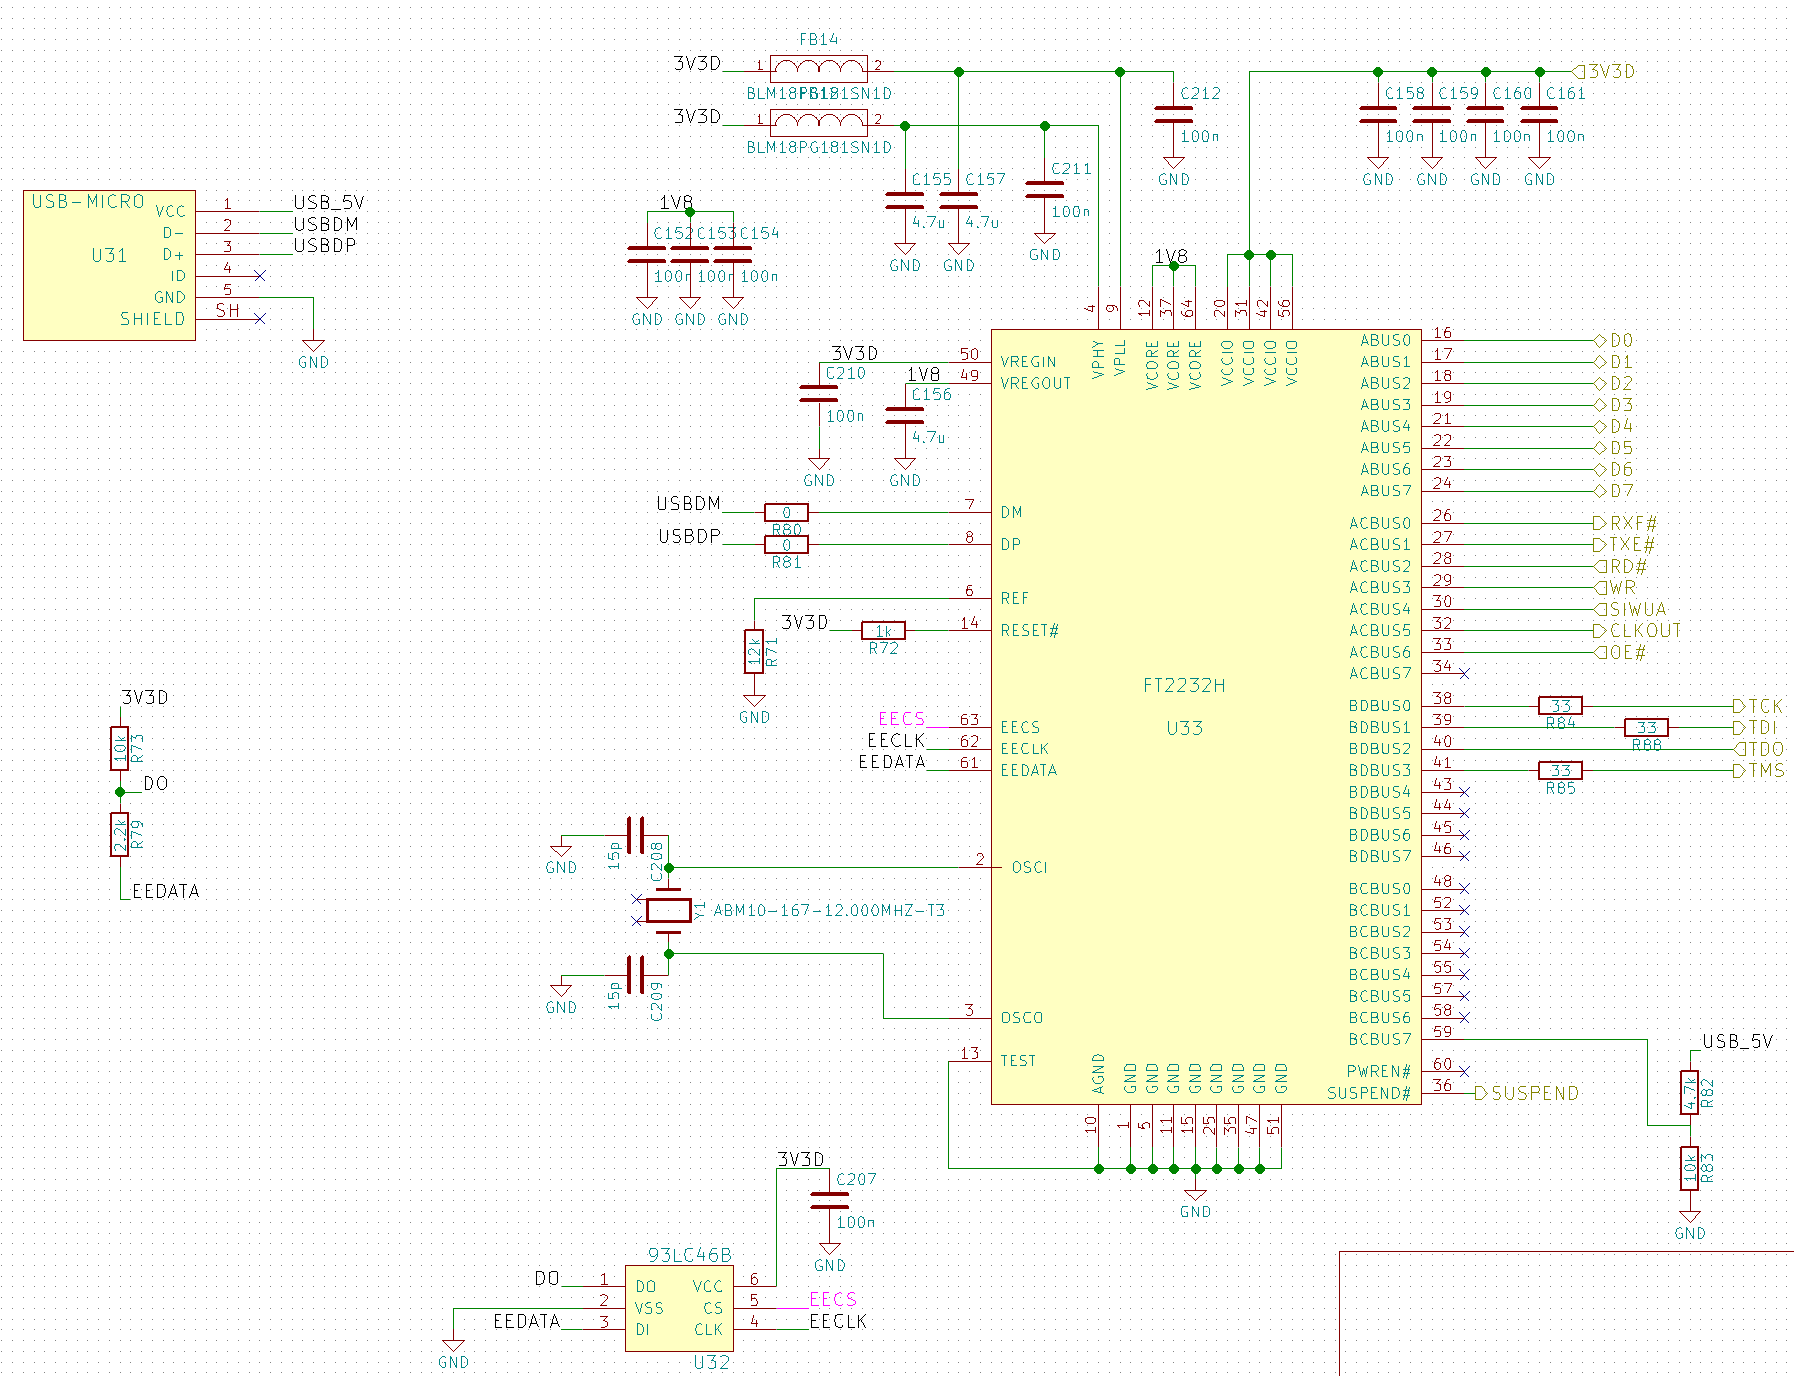
\includegraphics[width=\textwidth]{data/usb-ft2232.png}
  \caption{The configuration bit stream is loaded onto the FPGA using a USB-JTAG interface.}
  \label{fig:usb_ft2232}
\end{figure}

\subsection{93LC46B 1k EEPROM}
\label{sec:93lc46b}

\section{ADC}
\label{sec:adc}
\textit{\hyperlink{schematic.4}{schematic}}

\subsection{Overview}
\label{sec:adc-overview}

The ADC is used to digitize signals amplified by the IF \hyperref[sec:ada4940-2]{ADA4940-2}
differential amplifiers before sending them to the \hyperref[sec:xc7a15t-ftg256]{FPGA} for
processing.

\subsection{LTC2292}
\label{sec:ltc2292}

\subsubsection{Description}
\label{sec:ltc2292-description}

The \href{http://www.analog.com/media/en/technical-documentation/data-sheets/229321fa.pdf}{LTC2292}
is a 40MHz, 12-bit differential input ADC\@. This sets the Nyquist frequency at $20 \si{MHz}$, well
above the several hundred $\si{kHz}$ of the signal frequencies. Oversampling allows us to relax
anti-aliasing filter requirements, which improves bandwidth and resolution.

\subsubsection{Pinout}
\label{sec:ltc2292-pinout}

\label{tab:ltc2292-pinout}
\begin{tabularx}{\textwidth}{>{\hsize=.25\hsize} X >{\hsize=.25\hsize} XX}
        \caption{All LTC2292 ADC pin connections in logical groupings.} \\
        \toprule
        LABELS & PIN \#s & DESCRIPTION \\
        \midrule

        VDD & 7, 10, 18, 63 & The power supply required is 3.0V and each pin requires its own 0.1$\mu$F
        capacitor. When designing the PCB, ensure that each capacitor is placed as close to its
        corresponding pin as possible to minimize the trace inductance. The 3.0V signal itself
        is generated by using an LP5907 LDO regulator that takes in a 3.6V signal.\\
        OVDD & 39, 42 & The power supply for the output that the ADC feeds to, which is the FPGA and takes
        a 3.3V power supply. So, we connect this to the 3.3V power rail and bypass it with two 0.1$\mu$F
        capacitors, one for each pin. Again, each should be placed adjacent
        to their corresponding pins (39 and 42). \\
        CLKA, CLKB, MUX & 8, 9, 21 & Feeds a 40MHz clock signal to the device and specifies that the
        digitized channel A and B data should be multiplexed and pass through both output buses A and
        B. We leave B unconnected, so only bus A matters. Fig.~\ref{fig:ltc2292-multiplex} shows the
        timing for this. \\
        DA0-DA11 & 43-48, 51-56 & The digitized output data that contains the input data from both
        channels A and B, multiplexed. This is fed into the FPGA for
        processing. \\
        OFA & 57 & This pin is driven high when overflow or underflow occurs. Otherwise it is kept low. We
        export this to the FPGA, although it is not currently used by the FPGA logic. \\
        DB0-DB11 & 26-30, 33-39 & The channel B data bus. Since we multiplex everything through the
        channel A data bus, this data bus is redundant and therefore left unconnected. \\
        OFB & 40 & Similar to OFA, but for channel B. This is exported to the FPGA, but is also unused. \\
        VCMA, VCMB & 61, 20 & A 1.5V signal that is used to set the common-mode voltage of the IF
        differential amplifiers, whose outputs are sent to this ADC. They are each bypassed to GND with a
        2.2$\mu$F capacitor, which should be placed directly
        next to their respective pins. \\
        GND, OGND & 17, 64, 65, 31, 50 & The ADC power ground and output power ground, respectively. These
        can all be routed to the same ground plane. \\
        NC & 24-25, 41-42 & No connect. \\
        SHDNA, SHDNB, OEA, OEB & 59, 22, 58, 23 & These are input pins that are connected to the FPGA. The
        FPGA logic can ground both SHDNA and OEA to allow channel A to operate normally or bring them both
        high to put channel A in sleep mode. Channel B works the same
        way. \\
        SENSEA, SENSEB & 62, 19 & These are connected to VDD, which specifies that the input voltage range
        of the differential signals for both channels A and B is 1.5V $\pm$ 1V. 1.5V is the common-mode
        voltage and the channels allow a 2V range
        around that. \\
        MODE & 60 & Connecting mode to VDD specifies the output format as 2s complement and turns of the
        clock duty stabilizer, which is unnecessary because the input clock has a 50\% duty
        cycle. \\
        REFHA, REFLA, REFLB, REFHB & 3-6, 11-14 & These are the high and low reference for channels A and
        B, respectively. Their connection is specified exactly by the datasheet. It is critical that the
        0.1$\mu$F
        capacitor is placed as close to the pins as possible. \\
        AINA+, AINA-, AINB-, AINB+ & 1-2, 15-16 & The positive and negative differential inputs for
        channels A and B. \textbf{\{STARTINCOMPLETE\}} These lines have a capacitor between the positive
        and negative analog inputs, as well as capacitors connecting each line to GND. The capacitor value
        between the lines of 0.1$\mu$F is different from the suggested value of 12pF and the capacitors
        connecting the lines to GND are not suggested from the datasheet (see page 18 of the
        datasheet). Additionally, the resistance value of 49.9$\Omega$ differs from the suggested
        resistance of 25$\Omega$. Lastly, the negative output of the differential amplifier for channel A
        is feeding into the
        positive input line \textbf{\{END INCOMPLETE\}}. \\

        \bottomrule
\end{tabularx}

\begin{figure}[h]
        \centering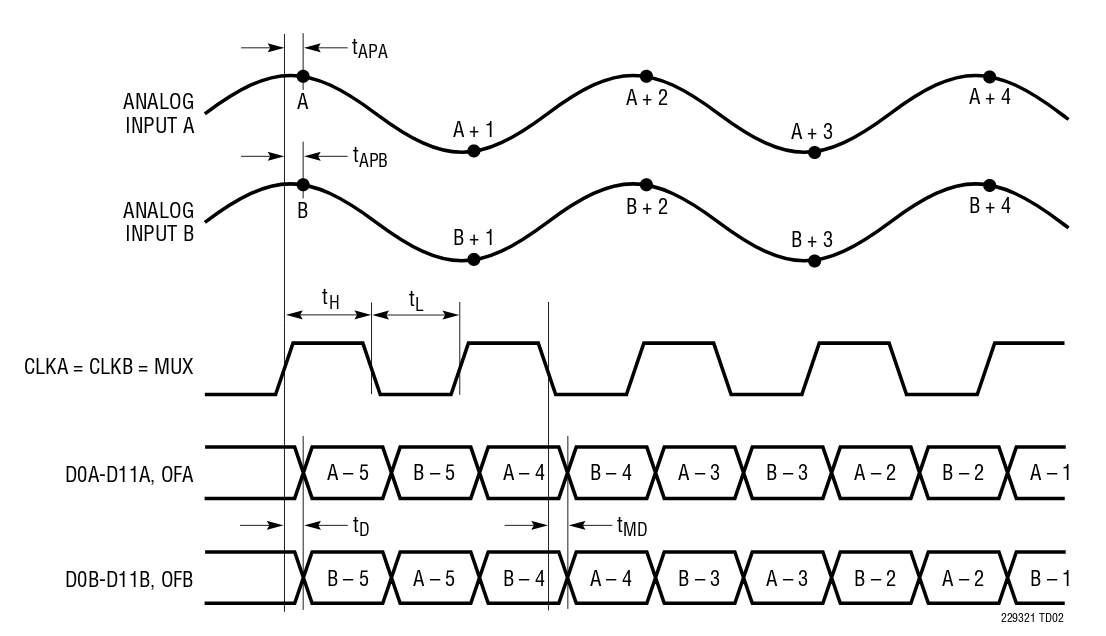
\includegraphics[width=0.75\textwidth]{data/LTC2292-multiplex.png}
        \caption{Multiplexed digital output bus timing for the LTC2292 ADC.}
        \label{fig:ltc2292-multiplex}
\end{figure}

\subsubsection{Component Selection}
\label{sec:ltc2292-component-selection}

The analog inputs employ anti-aliasing filters. The filters provide several benefits: (1) they
reduce aliasing by attenuating signals above the Nyquist frequency, (2) they limit wideband noise at
the input at the ADC input, which is important because the converter has a $575 \si{MHz}$ full-power
bandwidth, and (3) they isolate the \hyperref[sec:ada4940-2]{IF amplifier} from ADC noise at the
sampling frequency. Lastly, the capacitors act as a necessary charge source for the ADC input
capacitor. The two outer $100 \si{pF}$ capacitors (between the signal lines and ground) provide CMR
low-pass filtering with a cutoff frequency of $32 \si{MHz}$ (equation given in
Eq.~\ref{eq:anti-alias-cm-lp-filter}). The capacitor between the signal lines provides differential
low-pass filtering with a cutoff frequency of $16 \si{MHz}$. A
\href{https://e2e.ti.com/blogs_/archives/b/precisionhub/archive/2015/11/06/three-guidelines-for-designing-anti-aliasing-filters}{post
  from TI} explains this filtering. It's also important to keep the series resistor value low, since
the greater the resistance, the greater the Johnson noise.

\begin{equation}
        \label{eq:anti-alias-cm-lp-filter}
        f_{\text{c}} = \frac{1}{2 \pi R C}
\end{equation}

\subsubsection{PCB Layout}
\label{sec:ltc2292-pcb}



%%% Local Variables:
%%% mode: latex
%%% TeX-master: "fmcw-radar"
%%% End:

\section{TX}
\label{sec:tx}
\textit{\hyperlink{schematic.5}{schematic}}

\subsection{Overview}
\label{sec:tx-overview}

An RF frequency synthesizer and external VCO are used to generate a sine wave that is periodically
ramped from $5.3 \si{GHz}$ to $5.9 \si{GHz}$ over $1 \si{ms}$ with a $2 \si{ms}$ delay between
ramps. The signal is then power-amplified and a portion of the resulting signal is sent to an SMA
connector for transmission via an antenna and the remainder is kept on the board for mixing with the
received signal. Most of the power is directed for transmission.

\subsection{ADF4158 Frequency Synthesizer}
\label{sec:adf4158}

\subsubsection{Description}
\label{sec:adf4158-description}

The \href{http://www.analog.com/media/en/technical-documentation/data-sheets/ADF4158.pdf}{ADF4158}
is a 6.1GHz fractional-n frequency synthesizer. A block diagram describing its functionality is shown in
Figure~\ref{fig:adf4158-block-diagram}.

\begin{figure}[h]
        \centering
        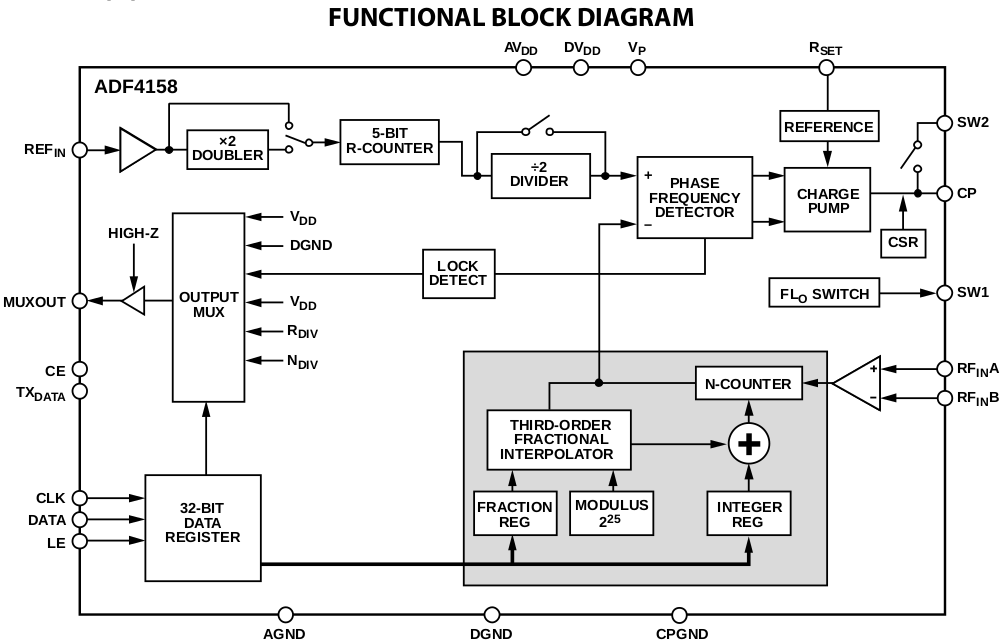
\includegraphics[width=0.75\textwidth]{data/adf4158-block-diagram.png}
        \caption{ADF4158 block diagram.}
        \label{fig:adf4158-block-diagram}
\end{figure}

The ADF4158 relies on an external VCO, described in \cref{sec:hmc431lp4rf}, whose output frequency
is given by Equation~\ref{eq:adf4158-rfout}. The output resolution is
$f_{\text{RES}} = f_{\text{PFD}}/2^{25}$ (see Equation~\ref{eq:adf4158-rfout} and its corresponding
parameter table for an explanation of $f_{\text{PFD}}$). The $2^{25}$ arises from the FRAC value
(set in registers 0 and 1) which is given 25 bits.

\begin{align}
  \text{RF}_{\text{OUT}} &= f_{\text{PFD}} \times \left(\text{INT} +
                           \left(\text{FRAC}/2^{25}\right)\right) \label{eq:adf4158-rfout} \\
  f_{\text{PFD}} &= \text{REF}_{\text{IN}} \times \left[\left(1 + D\right)/\left(R\times \left(1 +
                   T\right)\right) \right] \nonumber
\end{align}

\label{tab:adf4158-rfout-equation-vars}
\begin{tabularx}{\textwidth}{l X>{\raggedright\arraybackslash}X}
        \toprule
        \textbf{Parameter/Variable} & \textbf{Description} \\
        \midrule
        \endhead{}

        $\text{RF}_{\text{OUT}}$ & The VCO's output frequency. This is the frequency that's amplified for
        transmission. \\
        $f_{\text{PFD}}$ & The input frequency to the PFD post prescaling. In our case this is 20MHz. \\
        INT & The N counter that has a multiplicative effect on the VCO output frequency. \\
        FRAC & FRAC is the numerator of the fractional number added to INT. This is what distinguishes
        fractional-n synthesis from integer-n synthesis. It allows greater precision for the VCO
        output frequency without significantly increasing the prescalers and N counter. \\
        $\text{REF}_{\text{IN}} $ & The reference input frequency, which in our case is a 40MHz clock
        signal from the fanout buffer on the top level of the schematic. \\
        D & The doubler bit, which can be 0 or 1. If set to 1, the $\text{REF}_{\text{IN}}$ frequency is
        doubled before arriving at the R counter. \\
        R & The input prescaler. \\
        T & The divide- by-2 bit, which can be 0 or 1 and divides the frequency by 2 between the R
        prescaler and PFD. \\

        \bottomrule
\end{tabularx}

\subsubsection{Waveform Generation}
\label{sec:adf4158-waveform-generation}

The ADF4158 is capable of producing several different waveforms. The one used in this design is a
sawtooth ramp in frequency as a function of time, shown in
Figure~\ref{fig:adf4158-sawtooth-ramp}. There are 3 different parameters that determine the shape of
a ramp: (1) frequency deviation (the amount the frequency increases at each time step), (2) timeout
interval (the amount of time between each time step) and (3) the number of time steps. This is shown
diagrammatically in Figure~\ref{fig:adf4158-waveform-timing}. The equations governing these
parameters are given in Equation~\ref{eq:adf4158-waveform}. The number of steps is set directly in
register 6. In our configuration $f_{\text{DEV}} = 300\si{kHz}$ and $\text{Timer} = 0.5\si{\mu s}$,
which given that the number of steps is equal to 2000 and the starting frequency is 5.3GHz, the
sawtooth will ramp from 5.3GHz to 5.9GHz in 1ms. We also use a delay between bursts of
2ms. Equation~\ref{eq:adf4158-delay} is used to derive this.

\begin{align}
  f_{\text{DEV}} &= \left(f_{\text{PFD}}/2^{25}\right) \times \left(\text{DEV}\times
                   2^{\text{DEV\_OFFSET}}\right) \label{eq:adf4158-waveform} \\
  \text{Timer} &= \text{CLK}_1 \times \text{CLK}_2 \times \left(1/f_{\text{PFD}}\right) \nonumber
\end{align}

\label{tab:adf4158-waveform-equation-vars}
\begin{tabularx}{\textwidth}{l X>{\raggedright\arraybackslash}X}
        \toprule
        \textbf{Parameter/Variable} & \textbf{Description} \\
        \midrule

        \endhead

        $f_{\text{DEV}}$ & The frequency deviation for each frequency jump during ramp. \\
        $f_{\text{PFD}}$ & The input frequency to the PFD post prescaling. In our case this is 20MHz. \\
        DEV & A 16-bit value set in register 5. \\
        DEV\_OFFSET & A 4-bit word set in register 5. \\
        Timer & The time between each frequency hop. \\
        CLK\textsubscript{1} & A 12-bit clock divider set in register 2. \\
        CLK\textsubscript{2} & Another 12-bit clock divider set in register 4. \\

        \bottomrule
\end{tabularx}

\begin{equation}
        \label{eq:adf4158-delay}
        \text{Delay} = t_{\text{PFD}} \times \text{CLK}_1 \times \text{Delay Start Word}
\end{equation}

\label{tab:adf4158-delay-equation-vars}
\begin{tabularx}{\textwidth}{l X>{\raggedright\arraybackslash}X}
        \toprule
        \textbf{Parameter/Variable} & \textbf{Description} \\
        \midrule

        \endhead

        Delay & The delay between bursts. This is shown graphically in Figure~\ref{fig:adf4158-delay}. \\
        $f_{\text{PFD}}$ & The input frequency to the PFD post prescaling. In our case this is 20MHz. \\
        CLK\textsubscript{1} & A 12-bit clock divider set in register 2. \\
        Delay Start Word & A 12-bit value set in register 7. \\

        \bottomrule
\end{tabularx}

\begin{figure}[h]
        \centering
        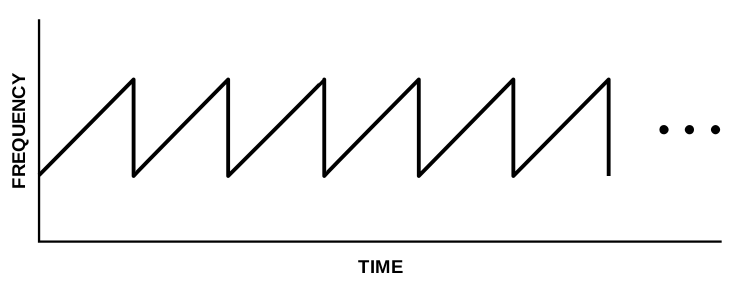
\includegraphics[width=0.5\textwidth]{data/adf4158-sawtooth-ramp.png}
        \caption{Sawtooth ramp.}
        \label{fig:adf4158-sawtooth-ramp}\end{figure}

\begin{figure}[h]
        \centering
        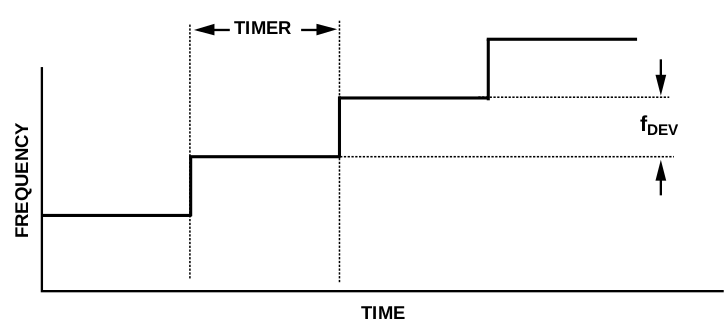
\includegraphics[width=0.5\textwidth]{data/adf4158-waveform-timing.png}
        \caption{Waveform timing.}
        \label{fig:adf4158-waveform-timing}
\end{figure}

\begin{figure}[h]
        \centering
        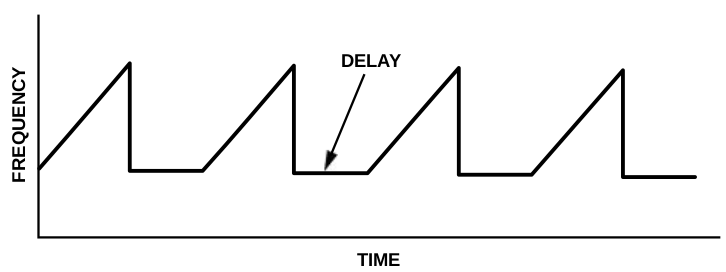
\includegraphics[width=0.5\textwidth]{data/adf4158-delay.png}
        \caption{Delay between ramps for sawtooth mode.}
        \label{fig:adf4158-delay}
\end{figure}

\subsubsection{Configuration Registers}
\label{sec:adf4158-config-regs}

The ADF4158 contains 8 configuration registers. The configurations are shown in the tables
below. All reserved bits should be set to 0. The control bits are the least significant 3 bits of
each register and are set to the register number for each register (e.g. register 0 is 000 and
register 1 is 001). I've left these out of the tables because their values are obvious.

\label{tab:adf4158-reg-map-0}
\begin{tabularx}{\textwidth}{l l l X>{\raggedright\arraybackslash}X}
        \caption{FRAC/INT REGISTER (R0) MAP} \\
        \toprule
        \textbf{Bits} & \textbf{Mnemonic} & \textbf{Value} & \textbf{DESCRIPTION} \\
        \midrule

        \endhead{}

        3--14 & FRAC(MSB) & 0 & This sets the 12 most significant bits of FRAC. We leave the fractional
        value at 0. \\
        15--26 & INT & 265 & This is the feedback, or N, counter. \\
        27--30 & MUXOUT Control & 15 & This enables ``readback to muxout'' which allows interrupting
        waveform generation and reading back the frequency at the time of
        interrupt. The functionality is not fully setup on the board(muxout
        connects to a DNP NMOS) and TX\_DATA, which can trigger the
        interrupt, is set to 0 by the FPGA HDL and left there. \\
        31 & Ramp On & 1 & This bit enables the ramp. \\

        \bottomrule
\end{tabularx}

\label{tab:adf4158-reg-map-1}
\begin{tabularx}{\textwidth}{l l l X>{\raggedright\arraybackslash}X}
        \caption{LSB FRAC REGISTER(R1) MAP} \\
        \toprule
        \textbf{Bits} & \textbf{Mnemonic} & \textbf{Value} & \textbf{DESCRIPTION} \\
        \midrule

        \endhead

        3-14 & Reserved & 0 & All reserved bits set to 0. \\
        15-27 & FRAC(LSB) & 0 & This sets the 13 least significant bits of FRAC. We leave the fractional
        value at 0. \\
        28-31 & Reserved & 0 & All reserved bits set to 0. \\

        \bottomrule
\end{tabularx}

\label{tab:adf4158-reg-map-2}
\begin{tabularx}{\textwidth}{l l l X>{\raggedright\arraybackslash}X}
        \caption{R-DIVIDER REGISTER(R2) MAP} \\
        \toprule
        \textbf{Bits} & \textbf{Mnemonic} & \textbf{Value} & \textbf{DESCRIPTION} \\
        \midrule

        \endhead

        3--14 & CLK\textsubscript{1} Divider & 10 & One of the determinants of the duration of a timestep in
        waveform generation. See
        \cref{sec:adf4158-waveform-generation} for more
        details. \\
        15--19 & R-Counter & 1 & This 5-bit segment is used to divide the frequency of the reference signal
        before it enters the PFD. We leave it at 1 and thus do not use it to
        divide the frequency. \\
        20 & Reference Doubler & 0 & We leave this at 0 and thus do not use the doubler to double the
        reference signal frequency before input to the PFD. The maximum input
        frequency for the PFD is 30MHz and so doubling our 20MHz signal (we
        used the divider to divide the 40MHz signal by 2) would violate this
        condition. \\
        21 & RDIV2 & 1 & Inserts a divide-by-2 toggle flip-flop between the R-counter and PFD. This
        provides a 50\% duty cycle that allows cycle slip reduction to be used which
        improves lock times. \\
        22 & Prescaler & 1 & The prescaler limits the INT value and through that the maximum frequency to
        3GHz. Since we have an INT value of 265 and our maximum frequency is almost
        double 3GHz we set this to 1. \\
        23 & Reserved & 0 & All reserved bits set to 0. \\
        24--27 & Charge Pump Current Setting & 0 & Sets the current to the minimum value which is 0.31mA
        and is the level necessary to use cycle slip reduction
        which we are. \\
        28 & CSR Enable & 1 & Enables cycle slip reduction which provides better lock times. \\
        29--31 & Reserved & 0 & All reserved bits are set to 0. \\

        \bottomrule
\end{tabularx}

\label{tab:adf4158-reg-map-3}
\begin{tabularx}{\textwidth}{l l l X>{\raggedright\arraybackslash}X}
        \caption{FUNCTION REGISTER(R3) MAP} \\
        \toprule
        \textbf{Bits} & \textbf{Mnemonic} & \textbf{Value} & \textbf{DESCRIPTION} \\
        \midrule

        \endhead{}

        3 & Counter Reset & 0 & When this is set to 1, the synthesizer counters are held in reset. For
        normal operation we set this to 0. \\
        4 & Charge Pump Three-State & 0 & Holds the charge pump in three-state mode if set to 1. For
        normal operation it must be set to 0. \\
        5 & Power-Down & 0 & Setting this to 1 powers down the device. Setting it to 0 allows normal
        operation. \\
        6 & PD Polarity & 1 & Set to 1 for positive VCO characteristics. Set to 0 for negative VCO
        characteristics. Since our VCO outputs a positive voltage signal we set this
        to 1. \\
        7 & LDP & 0 & Sets the minimum number of PFD cycles before a lock detect can be set. \\
        8 & FSK Enable & 0 & Disables FSK modulation. \\
        9 & PSK Enable & 0 & Disables PSK modulation. \\
        10-11 & Ramp Mode & 0 & Sets the waveform as a continuous sawtooth. \\
        12-13 & Reserved & 0 & All reserve bits are set to 0. \\
        14 & SD Reset & 0 & Setting this to 0 resets the $\Sigma-\Delta$ modulator on each write to
        register 0, which is the recommended operation. Setting this to 1 disables
        resetting the modulator. \\
        15 & N SEL & 0 & When set to 1, this creates an additional delay in setting INT and FRAC which can
        prevent the PLL overshooting. Since we set INT once and do not update it, this is
        not necessary and we leave it as 0. \\
        16-31 & Reserved & 0 & All reserve bits are set to 0. \\

        \bottomrule
\end{tabularx}

\label{tab:adf4158-reg-map-4}
\begin{tabularx}{\textwidth}{l l l X>{\raggedright\arraybackslash}X}
        \caption{TEST REGISTER(R4) MAP} \\
        \toprule
        \textbf{Bits} & \textbf{Mnemonic} & \textbf{Value} & \textbf{DESCRIPTION} \\
        \midrule

        \endhead{}

        3--6 & Reserved & 0 & All reserved bits are set to 0. \\
        7-18 & CLK\textsubscript{2} Divider & 1 & This is used to set the timeout interval in ramp
        generation. See
        \cref{sec:adf4158-waveform-generation}for more
        information. \\
        19-20 & CLK DIV Mode & 3 & This enables ramp divider mode, which specifies that
        CLK\textsubscript{1} and CLK\textsubscript{2} are used for ramp
        generation. \\
        21-22 & Readback to MUXOUT & 3 & Confusingly, this has been set to 3, which corresponds to neither
        of the supported values. Since we don't actually use the MUXOUT, this seems to be fine. If, at
        some point in the future, we do use the MUXOUT we will probably
        need to fix this. \\
        23-24 & Negative Bleed Current & 0 & This setting can help improve performance in the dead
        zone. We've disabled it. Note that this setting and readback
        to MUXOUT cannot simultaneously be enabled. To understand
        this setting better refer to \href{http://www.analog.com/media/en/technical-documentation/application-notes/AN-1154.pdf?doc=ADF4158.pdf}{AN-1154
          Application Note}. \\
        25 & Reserved & 0 & All reserved bits are set to 0. \\
        26-30 & $\Sigma-\Delta$ modulator mode & 0 & 0 enables this during normal operation. We can set it
        to 14 when FRAC=0. Even though we've set FRAC to 0,
        we have left this as 0 which seems strange. It
        shouldn't cause anything to malfunction, but may
        cause the ADF4158 to draw more power. We should
        experiment with setting this to 14 when using the
        actual board. \\
        31 & LE SEL & 0 & LE is the load enable pin which we use to load data onto the ADF4158's internal
        registers. Setting this to 0 enables the default operation of using the pin to
        set LE. Setting it to 1 would synchronize it with the reference signal. \\

        \bottomrule
\end{tabularx}

\label{tab:adf4158-reg-map-5}
\begin{tabularx}{\textwidth}{l l l X>{\raggedright\arraybackslash}X}
        \caption{DEVIATION REGISTER (R5) MAP} \\
        \toprule
        \textbf{Bits} & \textbf{Mnemonic} & \textbf{Value} & \textbf{DESCRIPTION} \\
        \midrule

        \endhead{}

        3--18 & Deviation Word & 31457 & This is used to set the size of successive frequency jumps during
        ramp. See \cref{sec:adf4158-waveform-generation} for more
        information. \\
        19--22 & Deviation Offset Word & 4 & This is also used to set the size of successive frequency
        jumps during ramp. See \cref{sec:adf4158-waveform-generation}
        for more information. \\
        23 & Deviation Select & 0 & Setting this bit to 1 is used for FSK as described on page 28 of the
        datasheet. Since we do not use FSK we leave this as 0. \\
        24 & Ramp 2 Enable & 0 & Setting this bit to 1 allows a second ramp with different settings than
        the first. We only need the first ramp. \\
        25 & FSK Ramp Enable & 0 & Setting this bit to 1 uses FSK. Again, we do not use FSK and so leave
        this bit as 0. \\
        26--27 & Interrupt & 0 & Sets the type of interrupt used to read the value of INT and FRAC of the
        ramp at a given moment. We don't read these values and therefore leave
        this as 0, which corresponds to interrupt off. \\
        28 & PAR Ramp & 0 & Setting this bit to 1 allows a parabolic ramp which we don't use. \\
        29 & Tx Ramp CLK & 0 & Setting this to 0 uses the clock divider (instead of the TX data clock) for
        clocking the ramp. \\
        30--31 & Reserved & 0 & \\

        \bottomrule
\end{tabularx}


\label{tab:adf4158-reg-map-6}
\begin{tabularx}{\textwidth}{l l l X>{\raggedright\arraybackslash}X}
        \caption{STEP REGISTER (R6) MAP} \\
        \toprule
        \textbf{Bits} & \textbf{Mnemonic} & \textbf{Value} & \textbf{DESCRIPTION} \\
        \midrule

        \endhead{}

        3--22 & Step Word & 2000 & This determines the number of steps in a ramp. To understand this see
        \cref{sec:adf4158-waveform-generation} on waveform generation. \\
        23 & Step SEL & 0 & This bit is used when 2 different ramps are needed (for instance with FSK). As
        we don't need this functionality we leave it off and set this bit to 0. \\
        24--31 & Reserved & 0 & \\

        \bottomrule
\end{tabularx}


\label{tab:adf4158-reg-map-7}
\begin{tabularx}{\textwidth}{l l l X>{\raggedright\arraybackslash}X}
        \caption{DELAY REGISTER (R7) MAP} \\
        \toprule
        \textbf{Bits} & \textbf{Mnemonic} & \textbf{Value} & \textbf{DESCRIPTION} \\
        \midrule

        \endhead{}

        3--14 & Delayed Start Word & 4000 & Sets the ramp start delay. We do not use a start delay, but we
        do use this to delay between ramps. \\
        15 & Delayed Start Enable & 0 & We do not use a start delay. \\
        16 & Delay Clock Select & 1 & Increases the period of the delay clock by multiplying the period of
        the PFD clock by CLK\textsubscript{1}. This creates an effective
        period of 500ns. \\
        17 & Ramp Delay & 1 & We enable a delay between ramp bursts. \\
        18 & Ramp Delay Fast Lock & 0 & Disables the ramp delay fast lock function. \\
        19--31 & Reserved & 0 & \\

        \bottomrule
\end{tabularx}

\label{tab:adf4158-pins}
\begin{tabularx}{\textwidth}{l l X>{\raggedright\arraybackslash}X}
        \caption{All ADF4158 pin connections.} \\
        \toprule
        \textbf{PIN} & \textbf{Mnemonic} & \textbf{DESCRIPTION} \\
        \midrule

        \endhead{}

        1 & CPGND & The charge pump ground, which we set to the same ground as the rest of the circuit. \\
        2, 3 & AGND & Prescaler ground; also set to common ground. \\
        4 & RF\textsubscript{IN} B & The complement to the VCO output. We couple this to ground with a
        small capacitor: in this case, 10pF. \\
        5 & RF\textsubscript{IN} A & The VCO output. This goes through prescaling and then becomes the PLL
        input signal. \\
        6, 7, 8 & AV\textsubscript{DD} & The positive power supply for the RF part of the PLL. This takes
        3.3V. \\
        9 & REF\textsubscript{IN} & The reference input, which is our 40MHz clock signal. \\
        10 & DGND & Digital ground. This uses the common ground. \\
        11 & SDGND & $\Sigma-\Delta$ modulator ground. \\
        12 & TX\textsubscript{DATA} & This pin can be used when employing FSK or PSK to transmit
        data. Since we are not using this we connect this pin to the FPGA
        but just set the value to GND. \\
        13 & CE & We must set this pin to high in order to enable the device. \\
        14 & CLK & A clock used to synchronize register configuration. \\
        15 & DATA & Serial data input to set the configuration registers. \\
        16 & LE & This pin is brought high in order to load data into the configuration registers. \\
        17 & MUXOUT & This allows internal parameters of the ADF4158 to be read externally. We don't
        currently use this in our design. \\
        18 & SDV\textsubscript{DD} & Power supply pin for the $\Sigma-\Delta$ modulator. We also set this
        to 3.3V. \\
        19 & DV\textsubscript{DD} & Power supply pin for the digital circuitry. Also 3.3V. \\
        20, 21 & SW1, SW2 & FIXME: These pins are used for the fast-locking feature, which we use in our
        design. The typical topologies for this are shown in
        Figure~\ref{fig:adf4158-fast-lock}. However, our design does not use either of
        these topologies. \\
        22 & V\textsubscript{P} & The charge pump power supply, which we set to 5V. \\
        23 & R\textsubscript{SET} & This pin sets the maximum charge pump current according to the
        equation $I_{\text{CPmax}}=25.5/R_{\text{SET}}$. We use
        5.49$\si{k\Omega}$ for the resistor which gives a charge pump current
        of 4.6mA. \\
        24 & CP & The charge pump output that is amplified and feeds into the VCO. Obviously, because this
        is a charge pump we need to place a bypass capacitor to ground before the
        amplifier. Here we use 51pF. \\
        25 & EPAD & This is connected to GND. \\

        \bottomrule
\end{tabularx}

\begin{figure}[h]
        \centering
        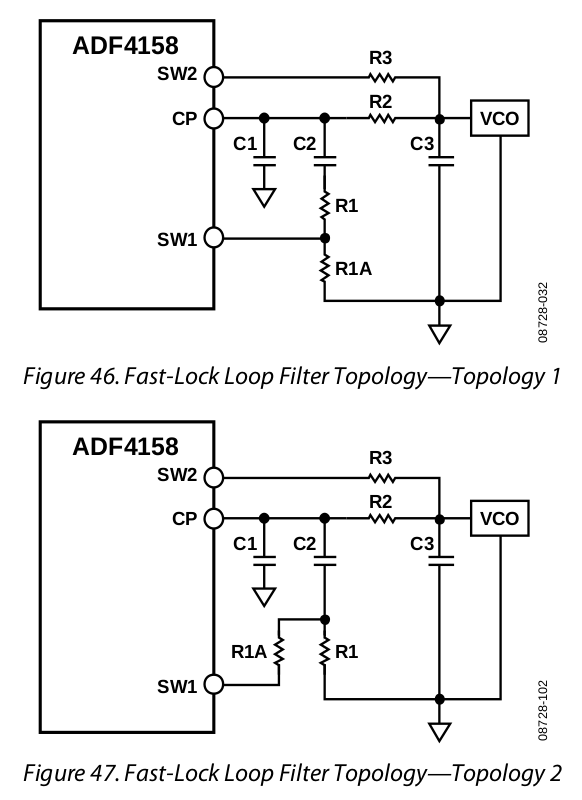
\includegraphics[width=0.5\textwidth]{data/adf4158-fast-lock.png}
        \caption{Fast lock topologies.}
        \label{fig:adf4158-fast-lock}
\end{figure}

\subsubsection{TLV2172 Operational Amplifier}
\label{sec:tlv2172-op-amp}

The \href{http://www.ti.com/lit/ds/symlink/tlv172.pdf}{TLV2172} op-amp is used to produce a gain of
2 to match the CP output of the ADF4158 to the VTUNE input of the VCO. This is necessary since the
charge pump supports a tune voltage of up to 5.5V but the VCO has a tune range of 0V to 10V. A
non-inverting amplifier configuration is used to produce the necessary gain.

\subsection{HMC431LP4RF VCO}
\label{sec:hmc431lp4rf}

The
\href{http://www.analog.com/media/en/technical_documentation/data_sheets/hmc431.pdf}{HMC431LP4RF} is
a radio-frequency VCO\@.

\subsection{DC4759J5020AHF Directional Coupler}
\label{sec:dc4759j5020ahf}

\subsubsection{Description}
\label{sec:dc4759j5020ahf-description}

The DC4759J5020AHF is a directional coupler with a $20 \si{dB}$ coupling factor, $0.17 \si{dB}$
insertion loss and $10.3 \si{dB}$ directivity. It is used to redirect some of the transmission power
back to the \hyperref[sec:adl5802]{mixer}'s local oscillator input. A directional coupler is a
4-terminal device, whose general form is shown in Fig.~\ref{fig:directional-coupler}. The coupling
factor gives the amount of input power that is redirected to the coupled port, the insertion loss
gives the amount of input power that is transmitted through to the output port and the directivity
is a measure of the coupler's ability to isolate the coupled and isolation ports. The actual
equations are given in Eq.~\ref{eq:coupling-factor}, Eq.~\ref{eq:insertion-loss} and
Eq.~\ref{eq:directivity}. In an ideal coupler, all input power is either transmitted through or
coupled. However, in all real directional couplers, some power is directed to the isolation port. In
our case $25.8 \si{dBm}$ is directed for transmission, $6 \si{dBm}$ is coupled, and $-4.3 \si{dBm}$
is sent to the isolated port.

\begin{figure}[h]
        \centering
        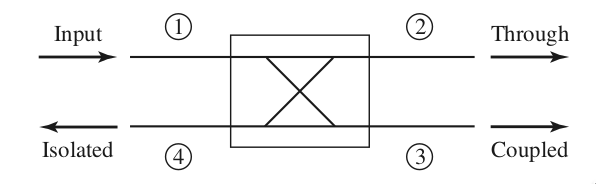
\includegraphics[width=0.5\textwidth]{data/directional-coupler}
        \caption{Directional coupler.}
        \label{fig:directional-coupler}
\end{figure}

\begin{equation}
        \label{eq:coupling-factor}
        C = 10 \log \frac{P_1}{P_3}
\end{equation}

\begin{equation}
        \label{eq:insertion-loss}
        L = 10 \log \frac{P_1}{P_2}
\end{equation}

\begin{equation}
        \label{eq:directivity}
        D = 10 \log \frac{P_3}{P_4}
\end{equation}

\subsubsection{PCB Layout}
\label{sec:dc4759j5020ahf-pcb}

The recommended PCB layout is shown in Fig.~\ref{fig:dc4759j5020ahf-pcb}, where the leftmost pads
correspond to the input and direct pins. All PCB traces leading from the pads should have a $50
\si{\Omega}$ characteristic impedance.

\begin{figure}[h]
        \centering
        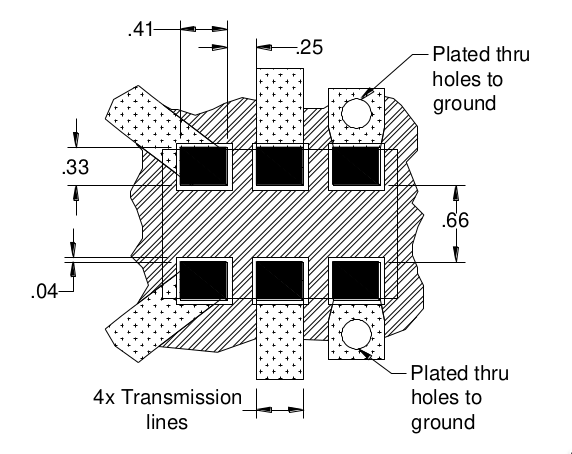
\includegraphics[width=0.3\textwidth]{data/dc4759j5020ahf-pcb}
        \caption{DC4759J5020AHF recommended PCB layout.}
        \label{fig:dc4759j5020ahf-pcb}
\end{figure}

\subsection{PD4859J5050S2HF Wilkinson Power Divider}
\label{sec:pd4859j5050s2hf}

\subsubsection{Description}
\label{sec:pd4859j5050s2hf-description}

The PD4859J5050S2HF is a Wilkinson power divider that equally divides the input power between the
two output ports. We use one after the \hyperref[sec:hmc431lp4rf]{VCO} to share its $2 \si{dBm}$
output power between the \hyperref[sec:se2567l]{power amplifier} and the RF\textsubscript{IN} port
of the \hyperref[sec:adf4158]{frequency synthesizer}.

\subsubsection{PCB Layout}
\label{sec:pd4859j50502shf-pcb}

The recommended layout is shown in Fig.~\ref{fig:pd4859j50502shf-pcb}. Ensure the location of the
external $100 \si{\Omega}$ 0603 resistor matches the location shown in the figure. All ports have a
$50 \si{\Omega}$ characteristic impedance which must be matched by the input and output traces.

\begin{figure}[h]
        \centering
        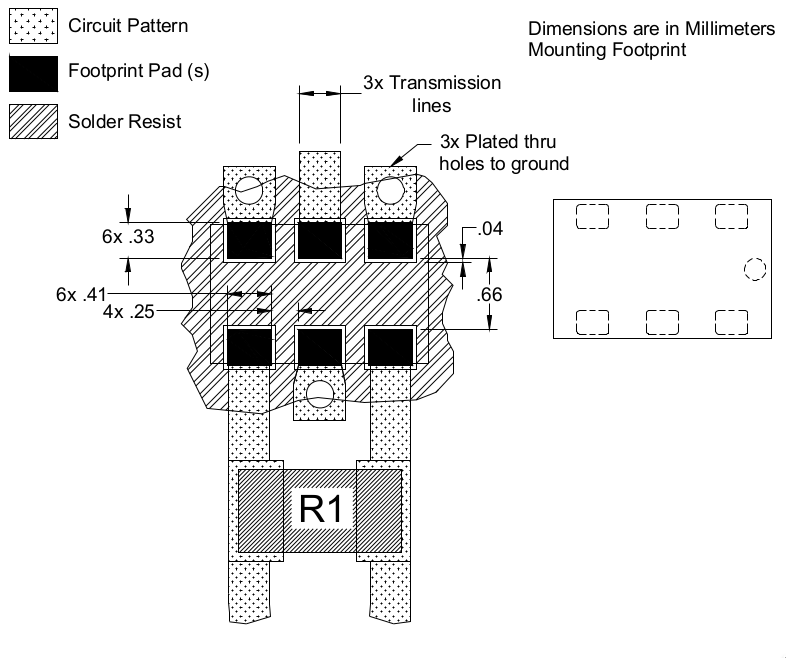
\includegraphics[width=0.5\textwidth]{data/pd4859j50502shf-pcb}
        \caption{PD4859J50502SHF recommended PCB layout. Note the location of the resistor.}
        \label{fig:pd4859j50502shf-pcb}
\end{figure}

\subsection{PAT1220 RF Attenuator}
\label{sec:pat1220}

\subsubsection{Description}
\label{sec:pat1220-description}

The PAT1220 is a simple resistive attenuator that can be used to preserve the shape of a signal but
decrease its power.

We use a $5 \si{dB}$ attenuator between the \hyperref[sec:hmc431lp4rf]{VCO} and
\hyperref[sec:se2567l]{power amplifier} in order to set the power amplifier's output power to its
typical value of $26 \si{dBm}$ as specified by the datasheet (it has a small-signal gain of
$32 \si{dB}$). This is enough power for a small radar (see~\cref{sec:distance}) and is sufficiently
below the $1 \si{dB}$ compression point, which should ensure good linearity.

I've placed a $3 \si{dB}$ attenuator between one of the \hyperref[sec:pd4859j5050s2hf]{Wilkinson
  power divider} outputs and the RF\textsubscript{IN} port of the \hyperref[sec:adf4158]{frequency
  synthesizer}. This shouldn't be strictly necessary, since the max power of the
RF\textsubscript{IN} port is $0 \si{dBm}$. However, using $-1 \si{dBm}$ would be playing it a bit
close. Additionally, the $2 \si{dBm}$ output of the VCO is a typical power output, not the max
power, which makes foregoing the attenuator even more dangerous. Finally, the RF\textsubscript{IN}
port supports an input power of as low as $-10 \si{dBm}$, so we have plenty of room on the downside.

The last attenuator ($6 \si{dB}$) is used at the coupled port of the
\hyperref[sec:dc4759j5020ahf]{directional coupler}, on its way to the local oscillator input of the
\hyperref[sec:adl5802]{mixer}. Again, the unattenuated $6 \si{dBm}$ should be ok (the max input
power of the LO is $10 \si{dBm}$). However, using the attenuator brings the LO power down to the
typical value specified by the mixer datasheet. To make sure our devices operate properly, we might
as well use the conditions recommended by the datasheet.

\subsubsection{PCB Layout}
\label{sec:pat1220-pcb-layout}

The recommended layout is shown in Fig.~\ref{fig:pat1220-pcb}. The ports are matched for a $50
\si{\Omega}$ characteristic trace impedance.

\begin{figure}[h]
        \centering
        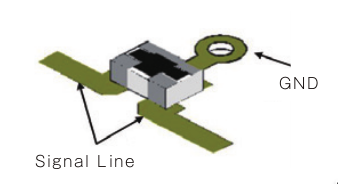
\includegraphics[width=0.25\textwidth]{data/pat1220-pcb}
        \caption{PAT1220 recommended PCB layout.}
        \label{fig:pat1220-pcb}
\end{figure}

\subsection{SE2567L Power Amplifier}
\label{sec:se2567l-power-amp}


%%% Local Variables:
%%% mode: latex
%%% TeX-master: "fmcw-radar"
%%% End:

\section{RX}
\label{sec:rx}

\subsection{SKY65404 LNA}
\label{sec:sky65404}



\subsection{TRF37A73 Gain Block}
\label{sec:trf37a73}



\subsubsection{PCB Layout}
\label{sec:trf37a73-pcb}


\begin{figure}[h]
        \centering
        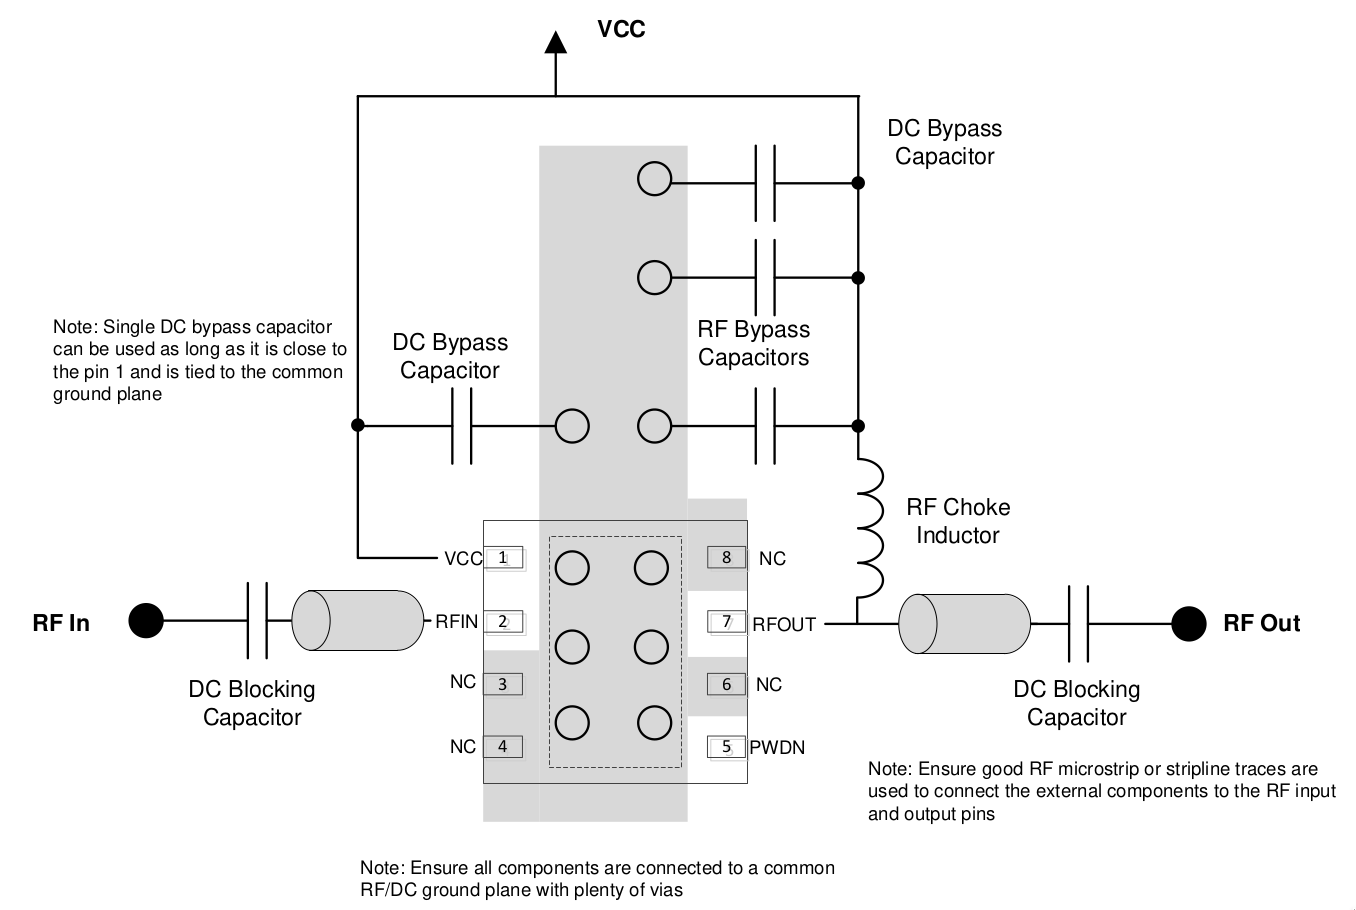
\includegraphics[width=\textwidth]{data/trf37a73-pcb}
        \caption{TRF37A73 recommended PCB layout.}
        \label{fig:trf37a73-pcb}
\end{figure}




The sheets RX1 and RX2 are identical. They each consist of two amplifiers connected in series, shown
in Figure~\ref{fig:rx-sch}. The first amplifier is a
\href{http://www.skyworksinc.com/uploads/documents/SKY65404_31_201512J.pdf}{SKY65404} LNA which
operates in the 4.9GHz-5.9GHz range, has a gain of 13dB, a NF of 1dB and a P1dB of -4dBm. It is
hooked up exactly as specified in the datasheet, with the addition of a ferrite bead filtering its
power supply.

\begin{figure}[h]
  \centering
  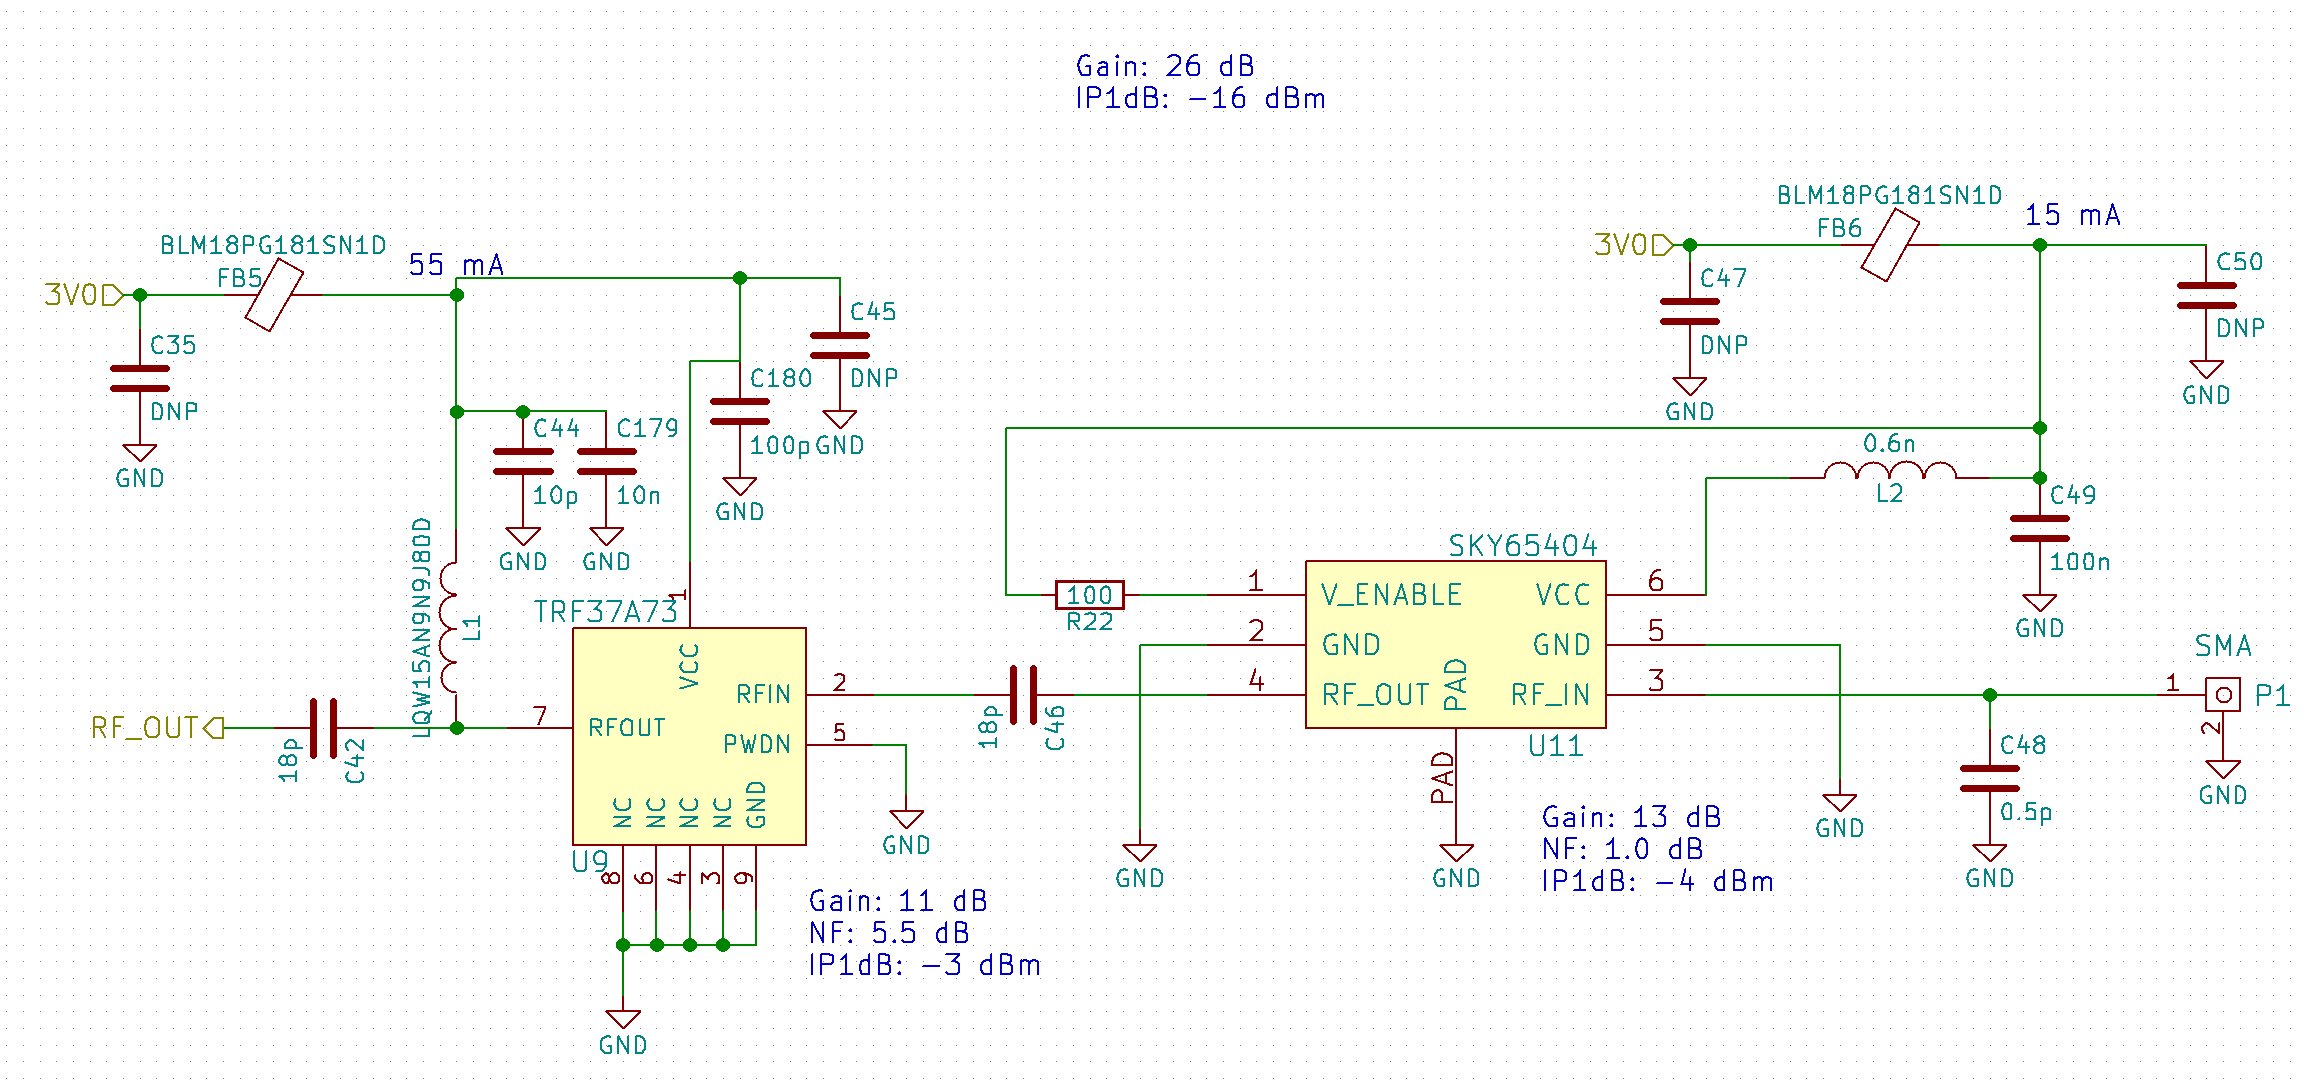
\includegraphics[width=\textwidth]{data/rx-sch.png}
  \caption{One of two RX schematic sheets. Both sheets are identical and consist of two amplifiers
    connected in series.}
  \label{fig:rx-sch}
\end{figure}

The second amplifier is a \href{http://www.ti.com/lit/ds/symlink/trf37a73.pdf}{TRF37A73} RF gain
amplifier. It is wired up as recommended in the datasheet, with the addition of a ferrite bead to
filter the power supply. Values for the various capacitors and inductor are left out of the
datasheet. A 100pF capacitor is used to short high frequency noise to the power supply, which is
typical of microwave devices. \textbf{\{START INCOMPLETE\}} I am not sure how the values for the RF
bypass capacitors, the inductor, and the DC blocking capacitors was chosen. Additionally, I'm not
sure how he arrives at a gain of 26dB, since I've read that gains in series should be additive (and
hence 24dB), and I'm not sure where the IP1dB value of -16dBm comes from \textbf{\{ENDINCOMPLETE\}}.

%%% Local Variables:
%%% mode: latex
%%% TeX-master: "fmcw-radar"
%%% End:

\section{Mixer}

\subsection{ADL5802}
\label{sec:adl5802}


The mixer schematic shown in Figure~\ref{fig:mixer-sch} is composed of three high-frequency baluns
that convert two rx and one local oscillator (the original transmitted signal) single-ended signal
into differential signals and then feed them into the mixer. The baluns are
\href{https://www.johansontechnology.com/datasheets/baluns/Balun_5400BL15B050.pdf}{5400BL15B050E}
and the mixer is
\href{http://www.analog.com/media/en/technical_documentation/data_sheets/ADL5802.pdf}{ADL5802}. The
mixer outputs the difference of the local oscillator frequency and each R input which ranges from
hundreds of kHz to a few MHz.

\begin{figure}[ht]
  \centering
  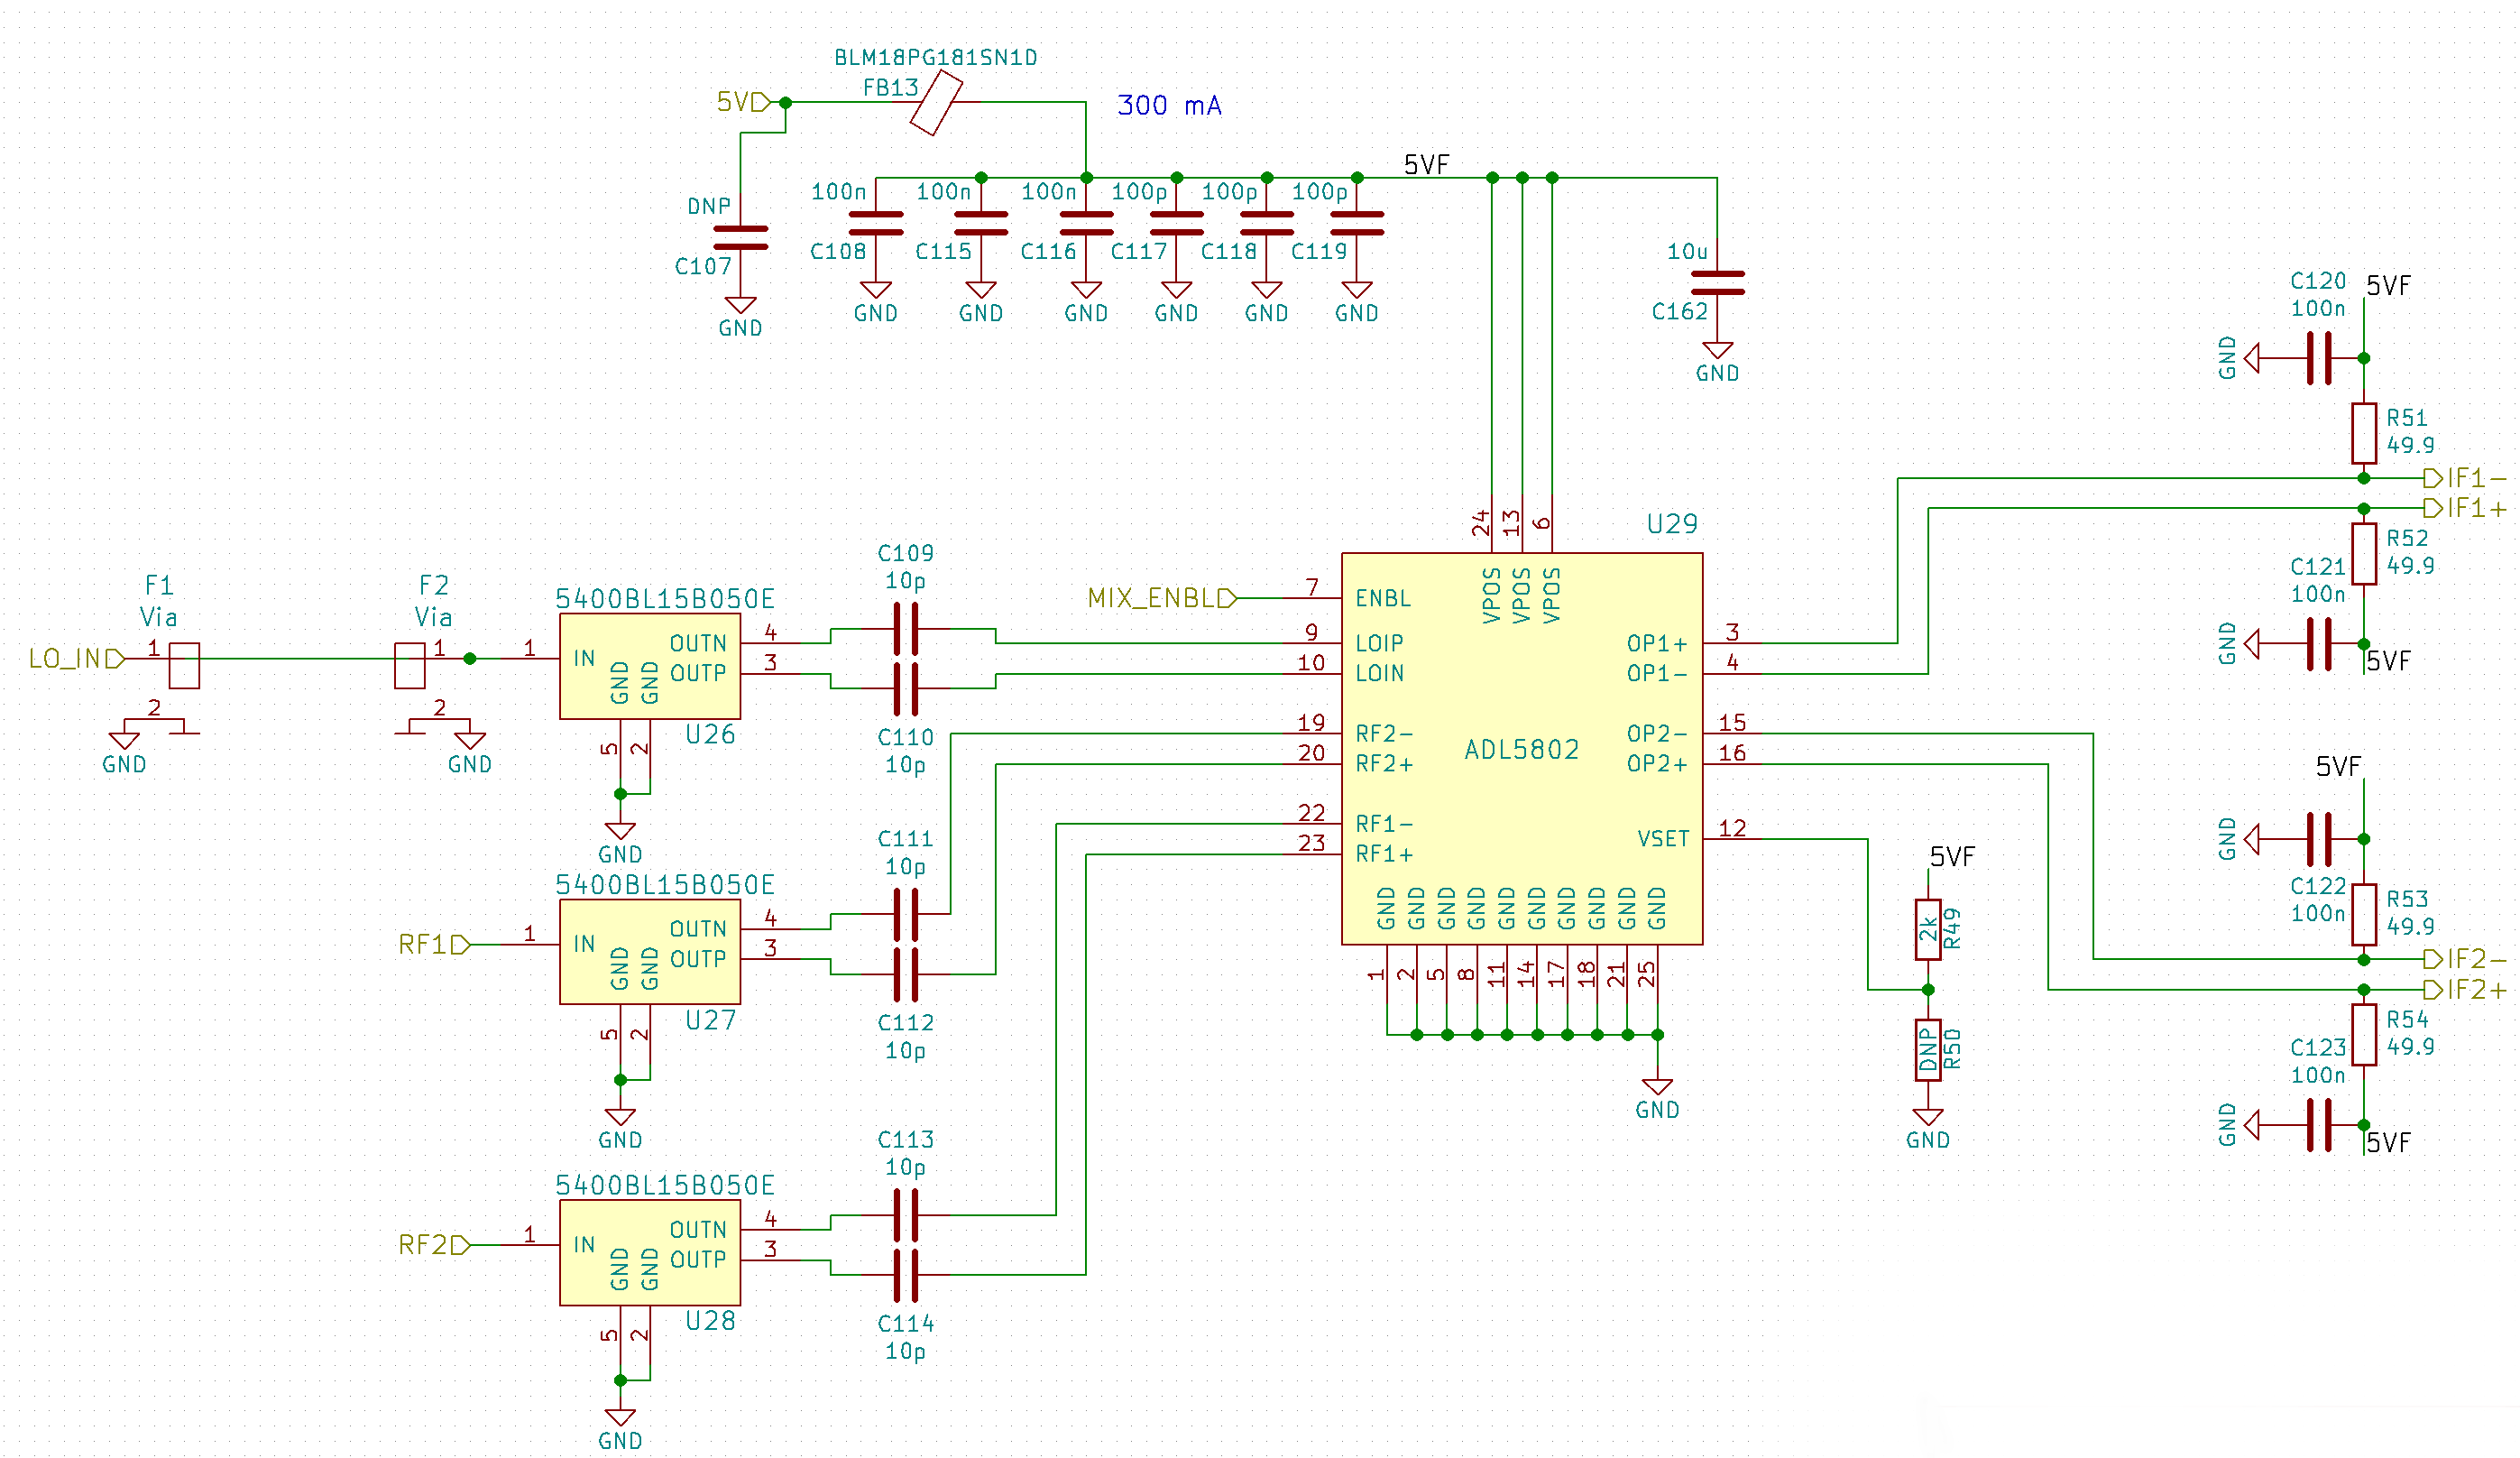
\includegraphics[width=\textwidth]{data/mixer-sch.png}
  \caption{The mixer schematic.}
  \label{fig:mixer-sch}
\end{figure}

The RF and LO input interfaces are designed for a differential input impedance of 50$\Omega$. This
is already the differential balanced impedance of the baluns, so we do not need to perform any
additional impedance matching at the inputs. The inputs require AC coupling and the datasheet
recommends 3pF coupling capacitors placed between the balun outputs and pin inputs. It also shows
that the positive balun output of the local oscillator should be hooked up to the positive pin
input.
\section{IF}
\label{sec:if}

The IF amplifier,
\href{http://www.analog.com/media/en/technical-documentation/data-sheets/ADA4940-1_4940-2.pdf}{ADA4940-2},
receives the output of the mixer, whose frequency is in the range of hundreds of kHz to a few MHz.

\subsection{ADA4940-2 IF Differential Amplifier}
\label{sec:ada4940-2}


\chapter{PCB}
\label{cha:pcb}

\section{General Layout}

The radar is constructed using a 4-layer board and uses both surfaces of the board. The front layer
contains nearly all of the board's components while the back layer contains a few surface mount
resistors and capacitors. The top layer primarily contains signal traces for top layer SMD
components. In particular, it connects many of the signal traces of the ADC to the FPGA, which is
placed next to it. Note, however, that most of the signal traces extending from the FPGA only start
on the top layer but travel through layer 3. The buck converters and subsequent linear regulators
are placed near the top of the board, not necessarily near the components they drive. In addition to
the large number of signal traces, the top copper layer contains a large ground plane around the
periphery of the board. The 2nd layer is entirely a ground plane. The 3rd layer is largely a ground
plane, although it also contains a significant number of traces extending from the FPGA as well as a
few other components. The 4th layer primarily contains large power planes for each of the different
voltages driving logic in the design. It is worth noting that even though it contains significant
power planes, it still has a ground plane that is the largest copper fill zone in this layer. The
PCB also has 3 large corner mounting vias with smaller vias placed in a circle in the large via's
annular ring. The reason for the small vias is to ensure a continued connection to GND (the mounting
vias are connected to GND) even if a screw thread strips too much copper from the main
via. Additionally, it helps prevent the PCB from being crushed if too much torque is used to tighten
the screw. The 4th corner is occupied by the connections to the DC barrel jack. Power rail traces
are made 0.5mm in width whereas signal traces are 0.2mm in width. Grounded vias are placed liberally
throughout the design. They have a diameter of 0.46mm and a drill hole size of 0.254mm. I've
included several screenshots of the PCB and highlighted important components
(Figures~\ref{fig:fmcw-layer1-layout}, ~\ref{fig:fmcw-layer1-gnd}, ~\ref{fig:fmcw-layer2-gnd},
~\ref{fig:fmcw-layer3-gnd}, ~\ref{fig:fmcw-layer4-gnd}, ~\ref{fig:fmcw-layer4-12v},
~\ref{fig:fmcw-layer4-3v6}, ~\ref{fig:fmcw-layer4-3v0}, ~\ref{fig:fmcw-layer4-3v3a},
~\ref{fig:fmcw-layer4-3v3d}, ~\ref{fig:fmcw-layer4-5v}, ~\ref{fig:fmcw-layer4-5vf}).

\begin{figure}[h]
        \centering
        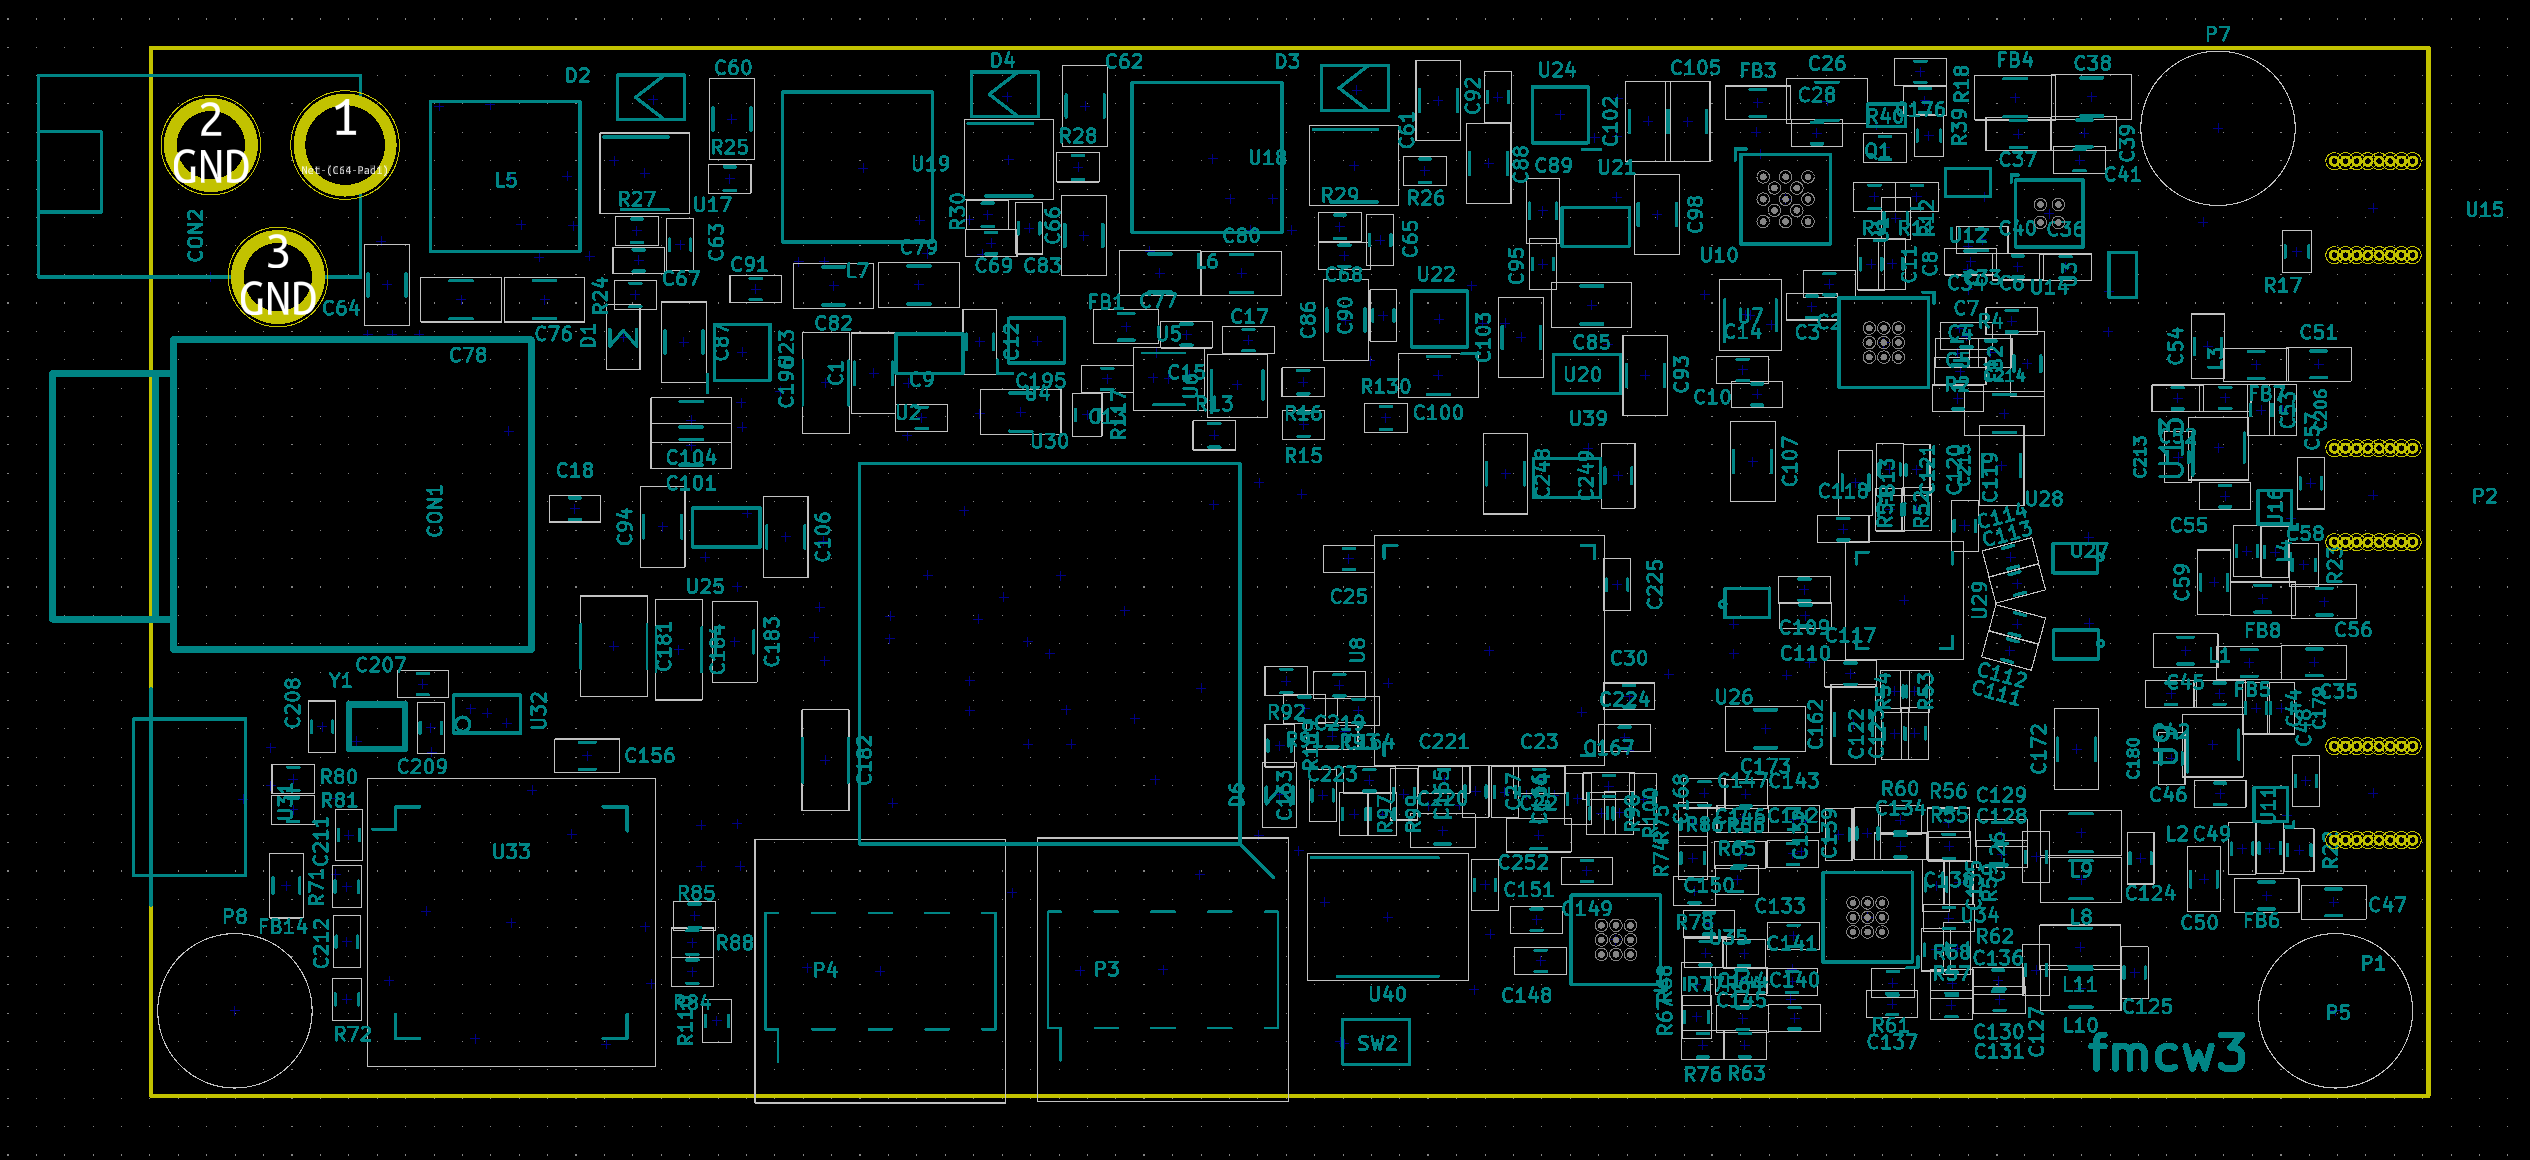
\includegraphics[width=\textwidth]{data/fmcw-layer1-layout.png}
        \caption{\textbf{Board layout}. The top left of the board is where the power source (barrel
          jack) is connected. The output of the 12V power source is connected to a power plane at
          the top left-middle of the board, that feeds into the buck converters. Large inductors
          connected to the buck converters are placed adjacent to their corresponding buck
          converters. The outputs of the buck converters feed into linear regulators that are mostly
          placed directly below the buck converters. This is also the region where the main crystal
          oscillator is placed and its associated fan-out buffer. Transmission circuitry (the
          frequency synthesizer and some RF amplifiers) are placed at the upper right side of the
          board near the antenna connectors which are placed on the right side of the
          board. Circuitry for signal reception are placed along the right side, adjacent to the
          antenna connectors. The mixer is placed slight inward from here, vertically centered but
          toward the right side of the board. Below this are intermediate frequency op-amps that
          feed the mixed signal into an ADC located just above it and to the left (U8). Located just
          to the left of the IF amplifiers and below the ADC is a flash memory IC (U40) which feeds
          data to the FPGA (U30), located just to the left of the ADC. Connectors below the FPGA (P3
          and P4) can be used to externally monitor the FPGA. In the bottom left of the board is a
          component to convert USB data to UART data to configure the FPGA as well as a micro USB
          connection to connect to a host computer. On the left side of the board between the USB
          connection and barrel jack is a SD card reader that stores data that can be read back out
          the FPGA.}
        \label{fig:fmcw-layer1-layout}
\end{figure}

\begin{figure}[h]
        \centering
        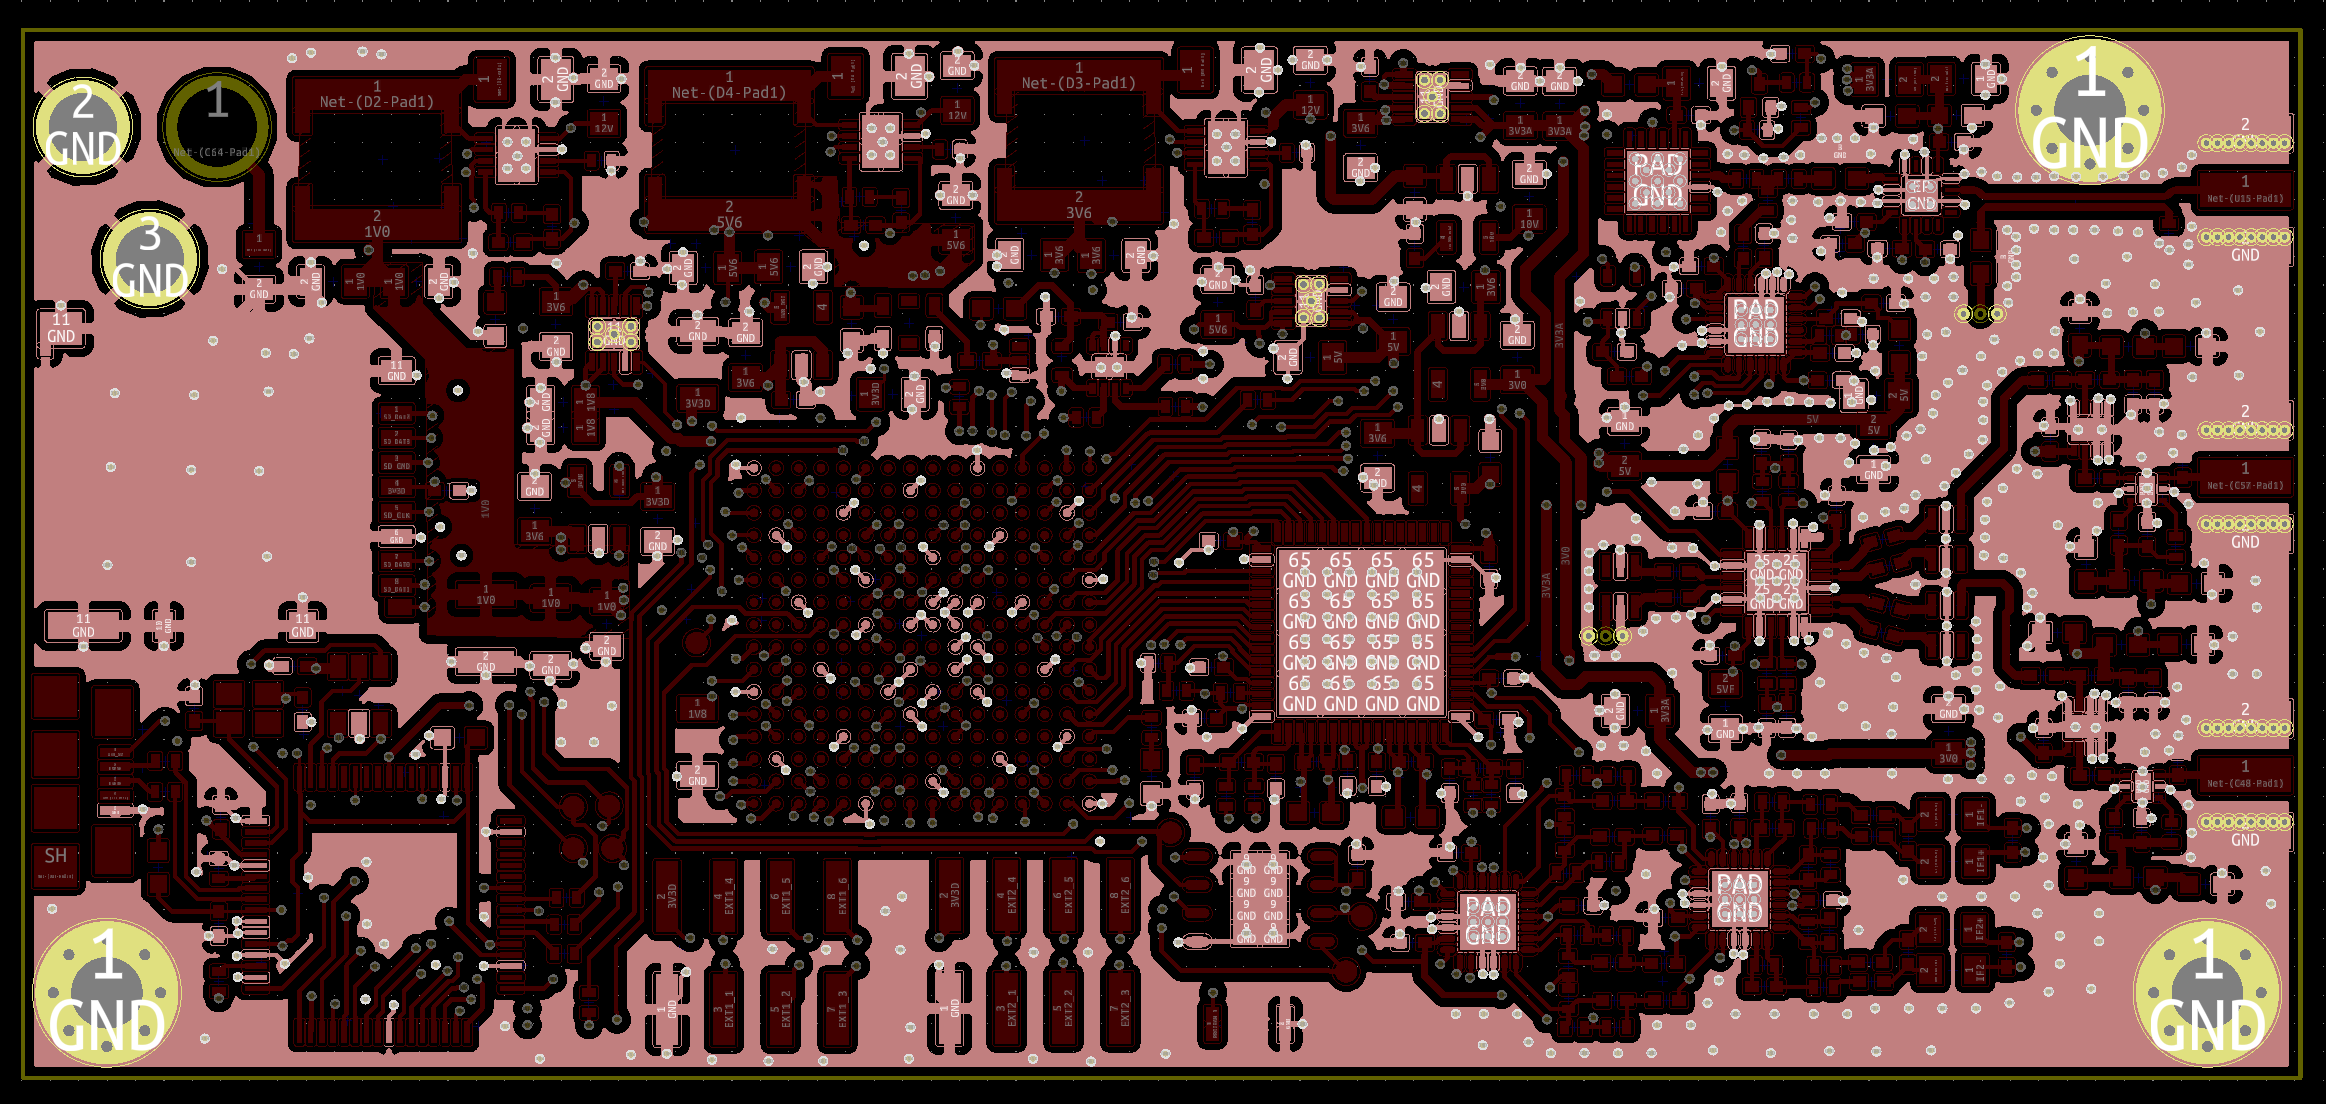
\includegraphics[width=\textwidth]{data/fmcw-layer1-gnd.png}
        \caption{A significant portion of layer 1 is a ground plane and the other large part of it
          is signal traces connecting components. There is also a small 1V power plane toward the
          upper left not highlighted here.}
        \label{fig:fmcw-layer1-gnd}
\end{figure}

\begin{figure}[h]
        \centering
        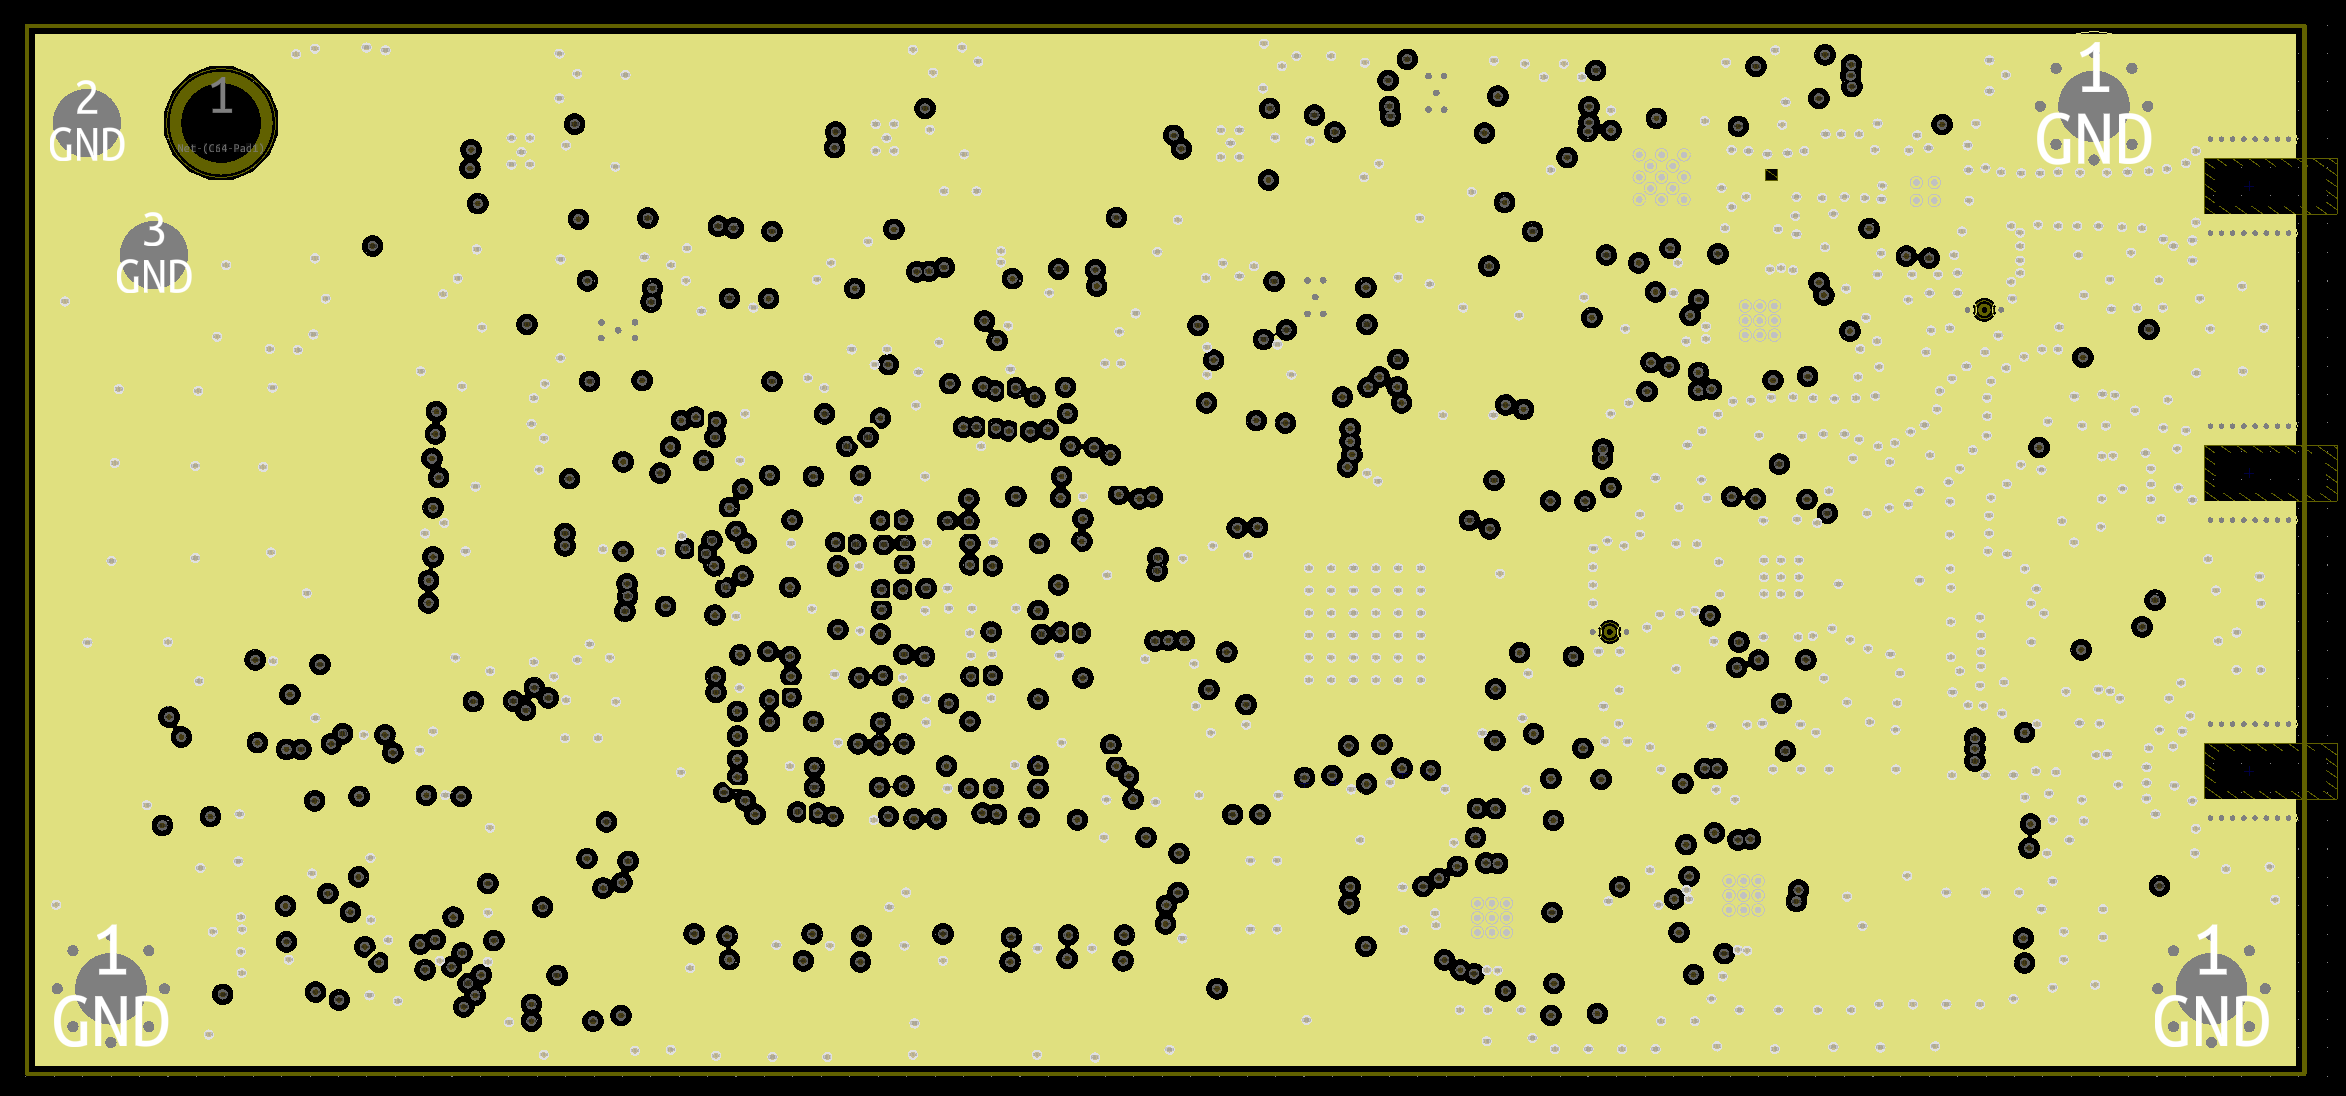
\includegraphics[width=\textwidth]{data/fmcw-layer2-gnd.png}
        \caption{All of layer 2 is a ground plane.}
        \label{fig:fmcw-layer2-gnd}
\end{figure}

\begin{figure}[h]
        \centering
        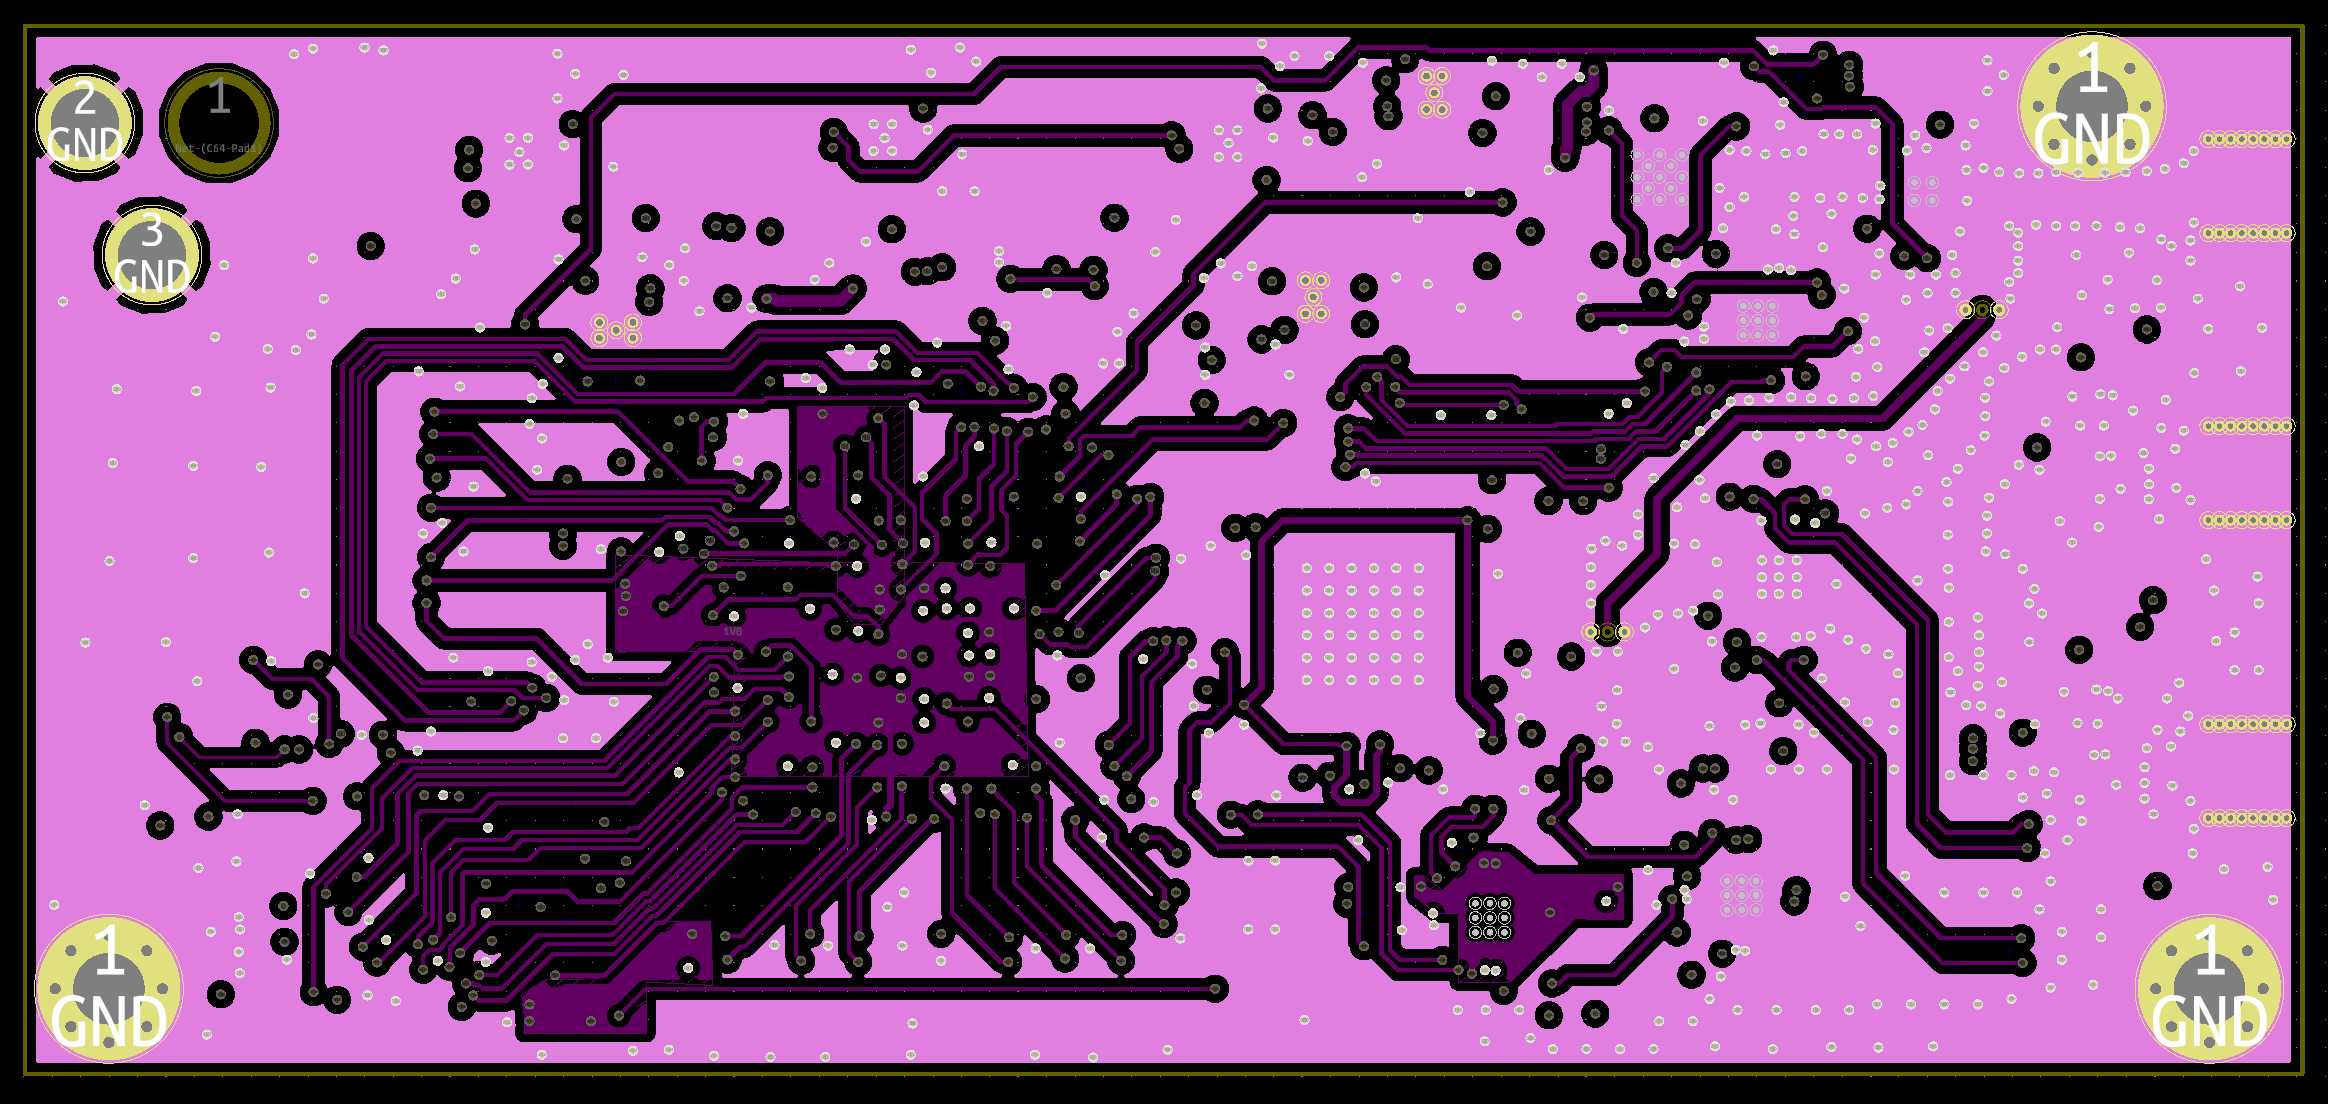
\includegraphics[width=\textwidth]{data/fmcw-layer3-gnd.png}
        \caption{Most of layer 3 is a ground plane but there are also a substantial number of trace
          connecting to the FPGA. It does also contain 1V an 3.3V power planes.}
        \label{fig:fmcw-layer3-gnd}
\end{figure}

\begin{figure}[h]
        \centering
        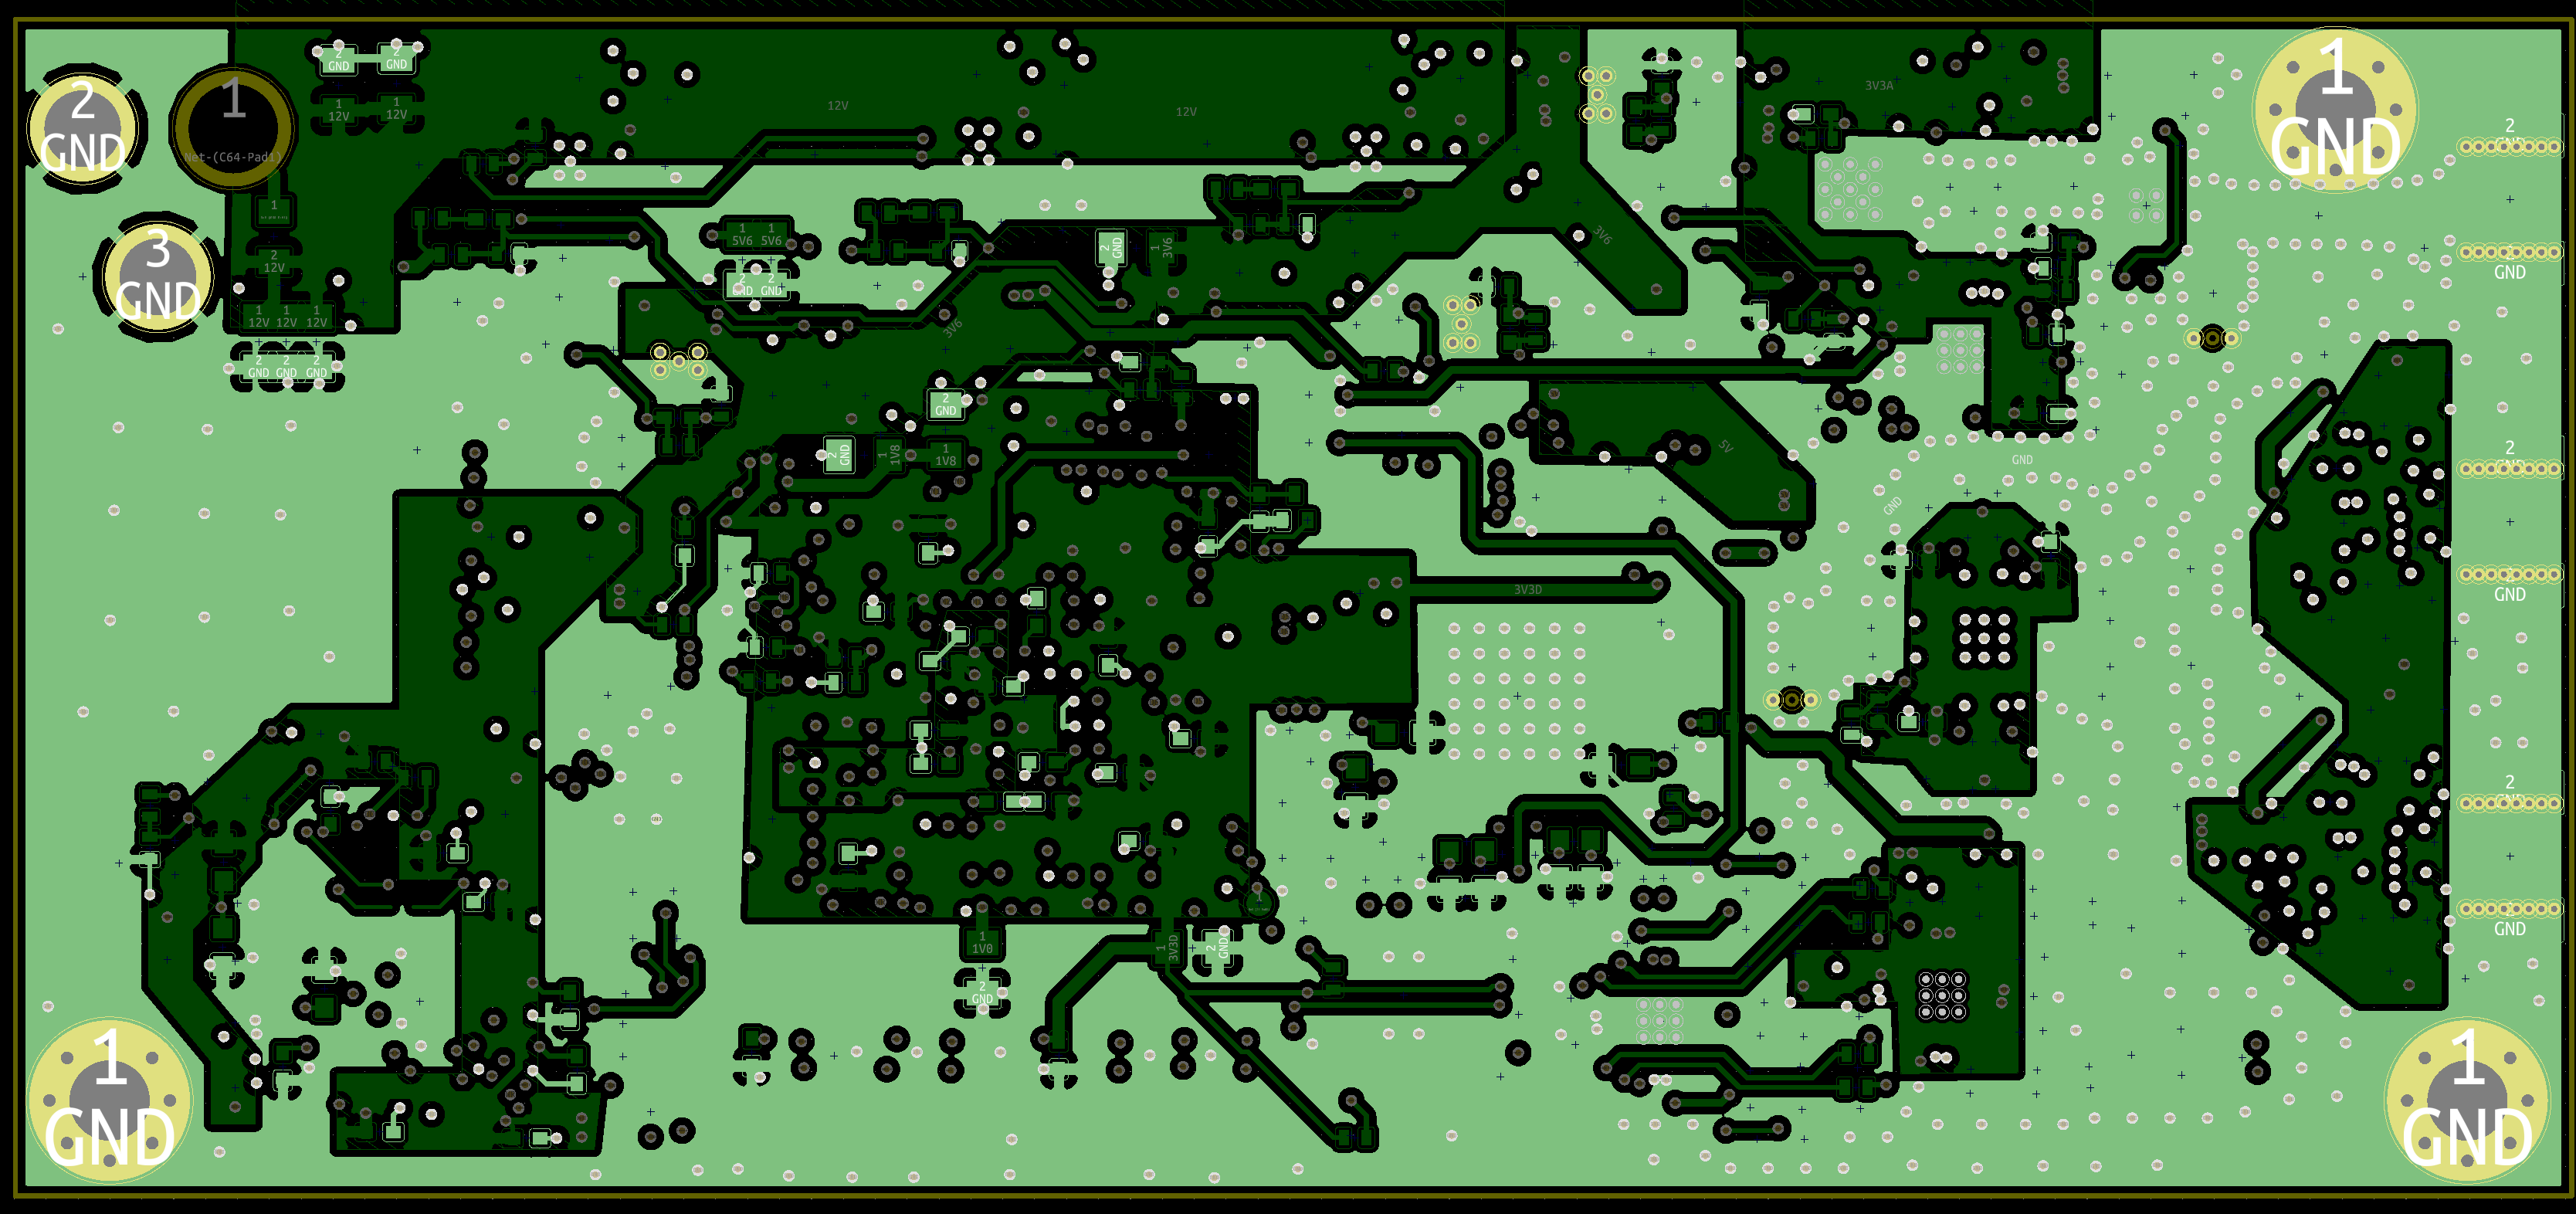
\includegraphics[width=\textwidth]{data/fmcw-layer4-gnd.png}
        \caption{The 4th layer of the PCB contains a large ground plane with many vias
          interspersed.}
        \label{fig:fmcw-layer4-gnd}
\end{figure}

\begin{figure}[h]
        \centering
        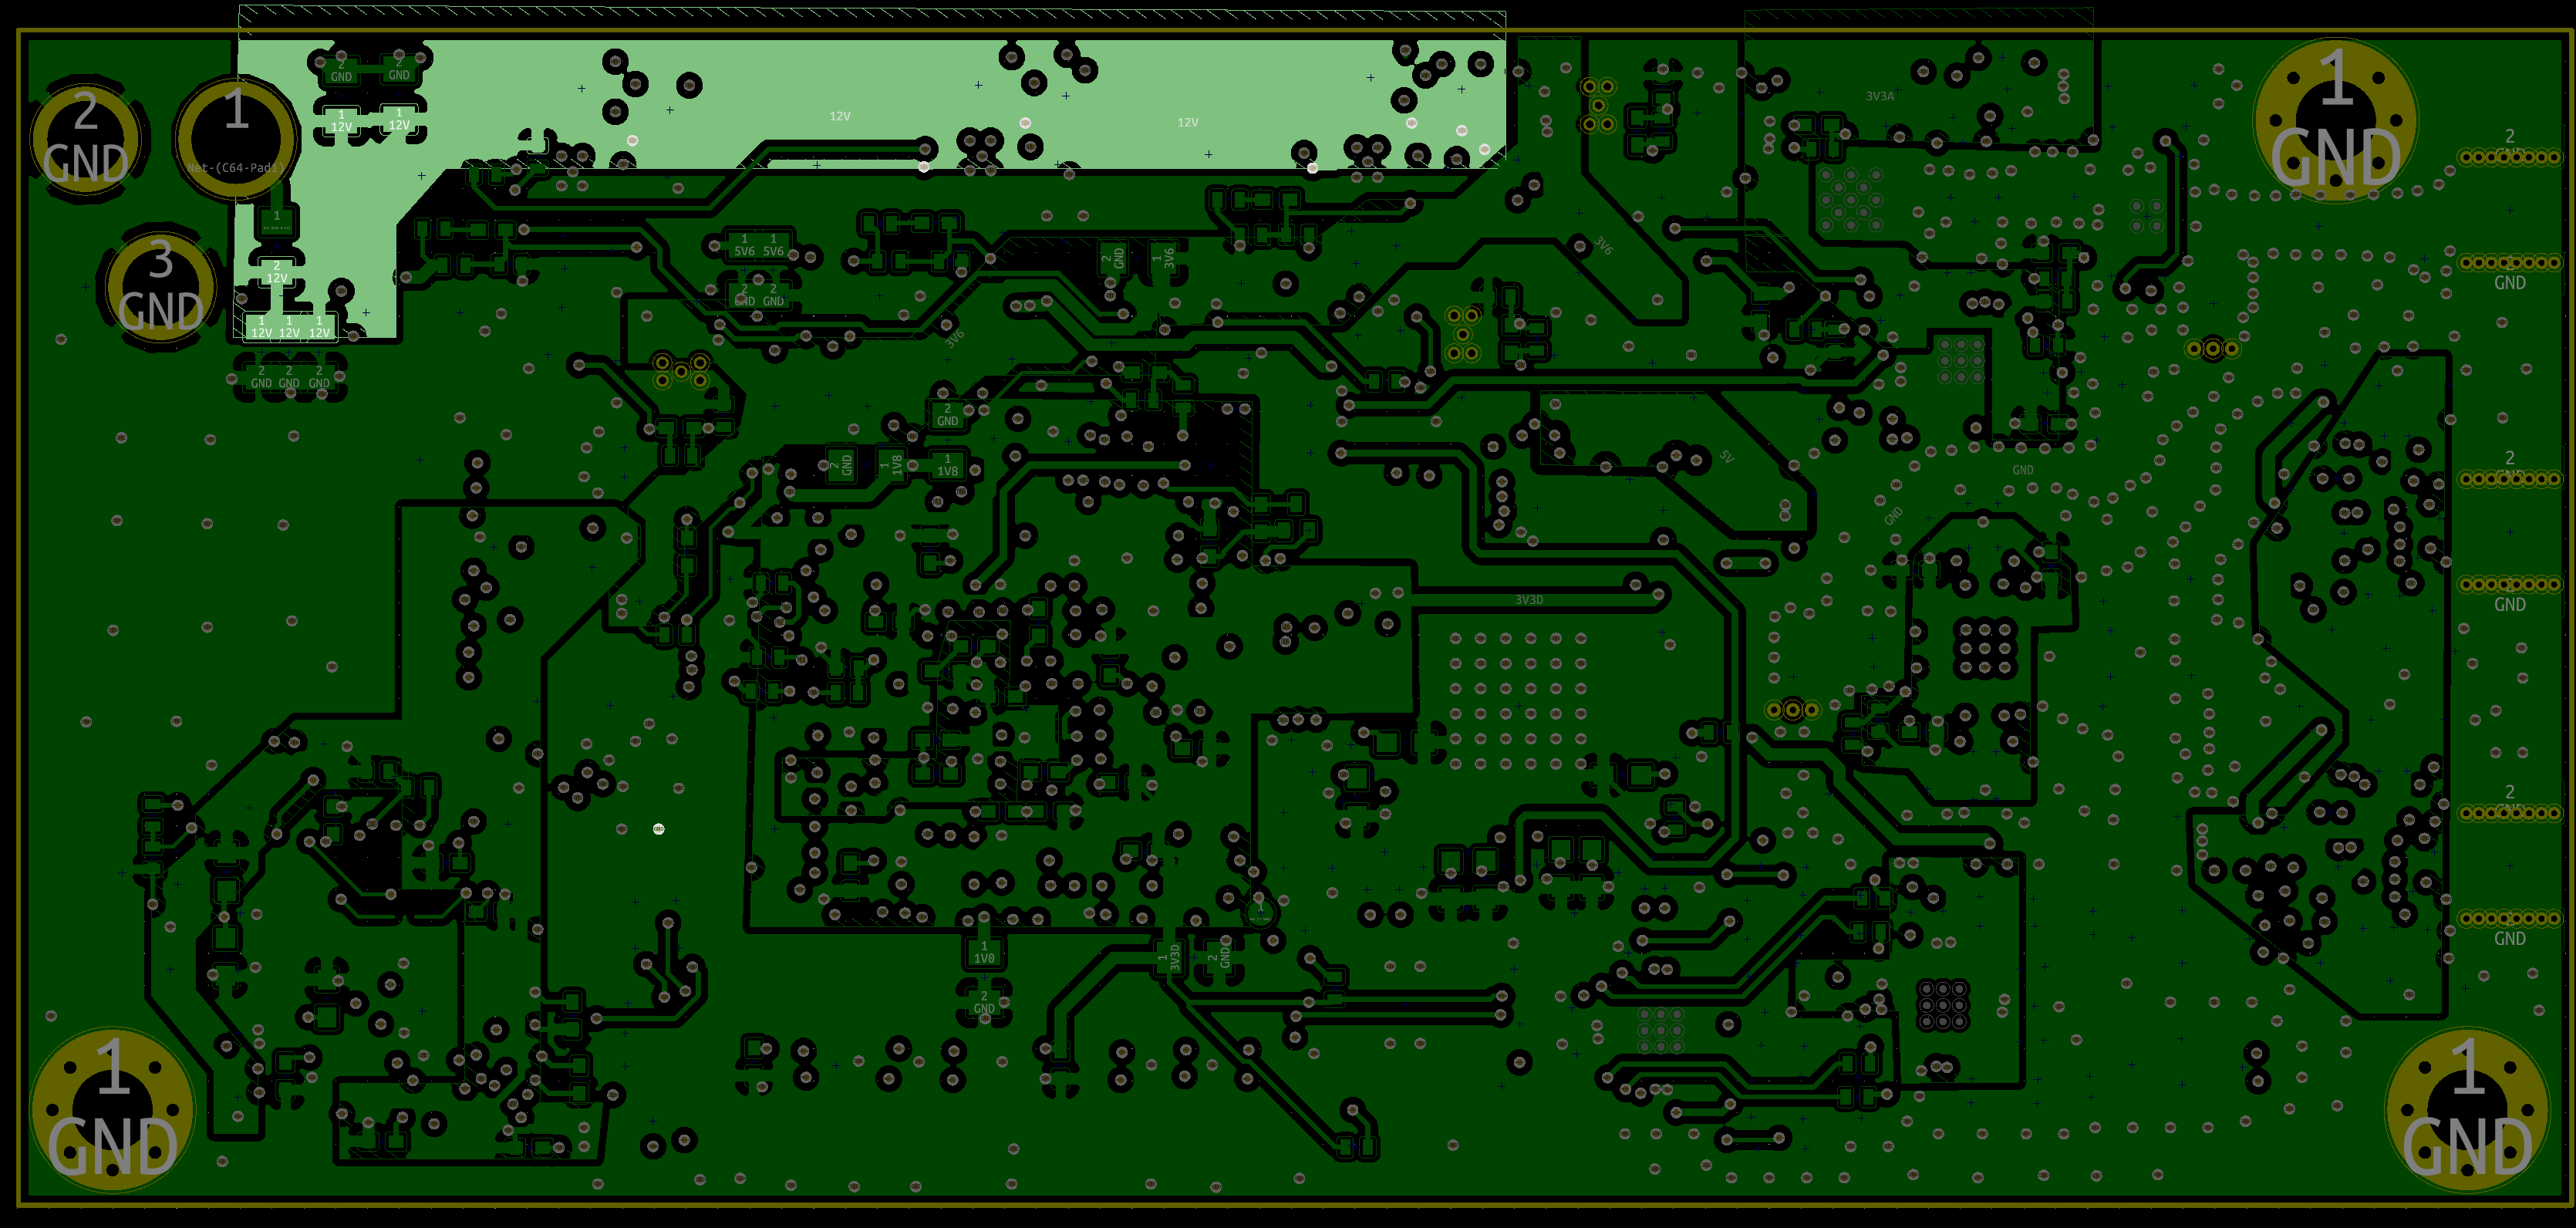
\includegraphics[width=\textwidth]{data/fmcw-layer4-12v.png}
        \caption{The 12V power plane is located at the top of the board adjacent to the D barrel
          jack and the buck converters it feeds.}
        \label{fig:fmcw-layer4-12v}
\end{figure}

\begin{figure}[h]
        \centering
        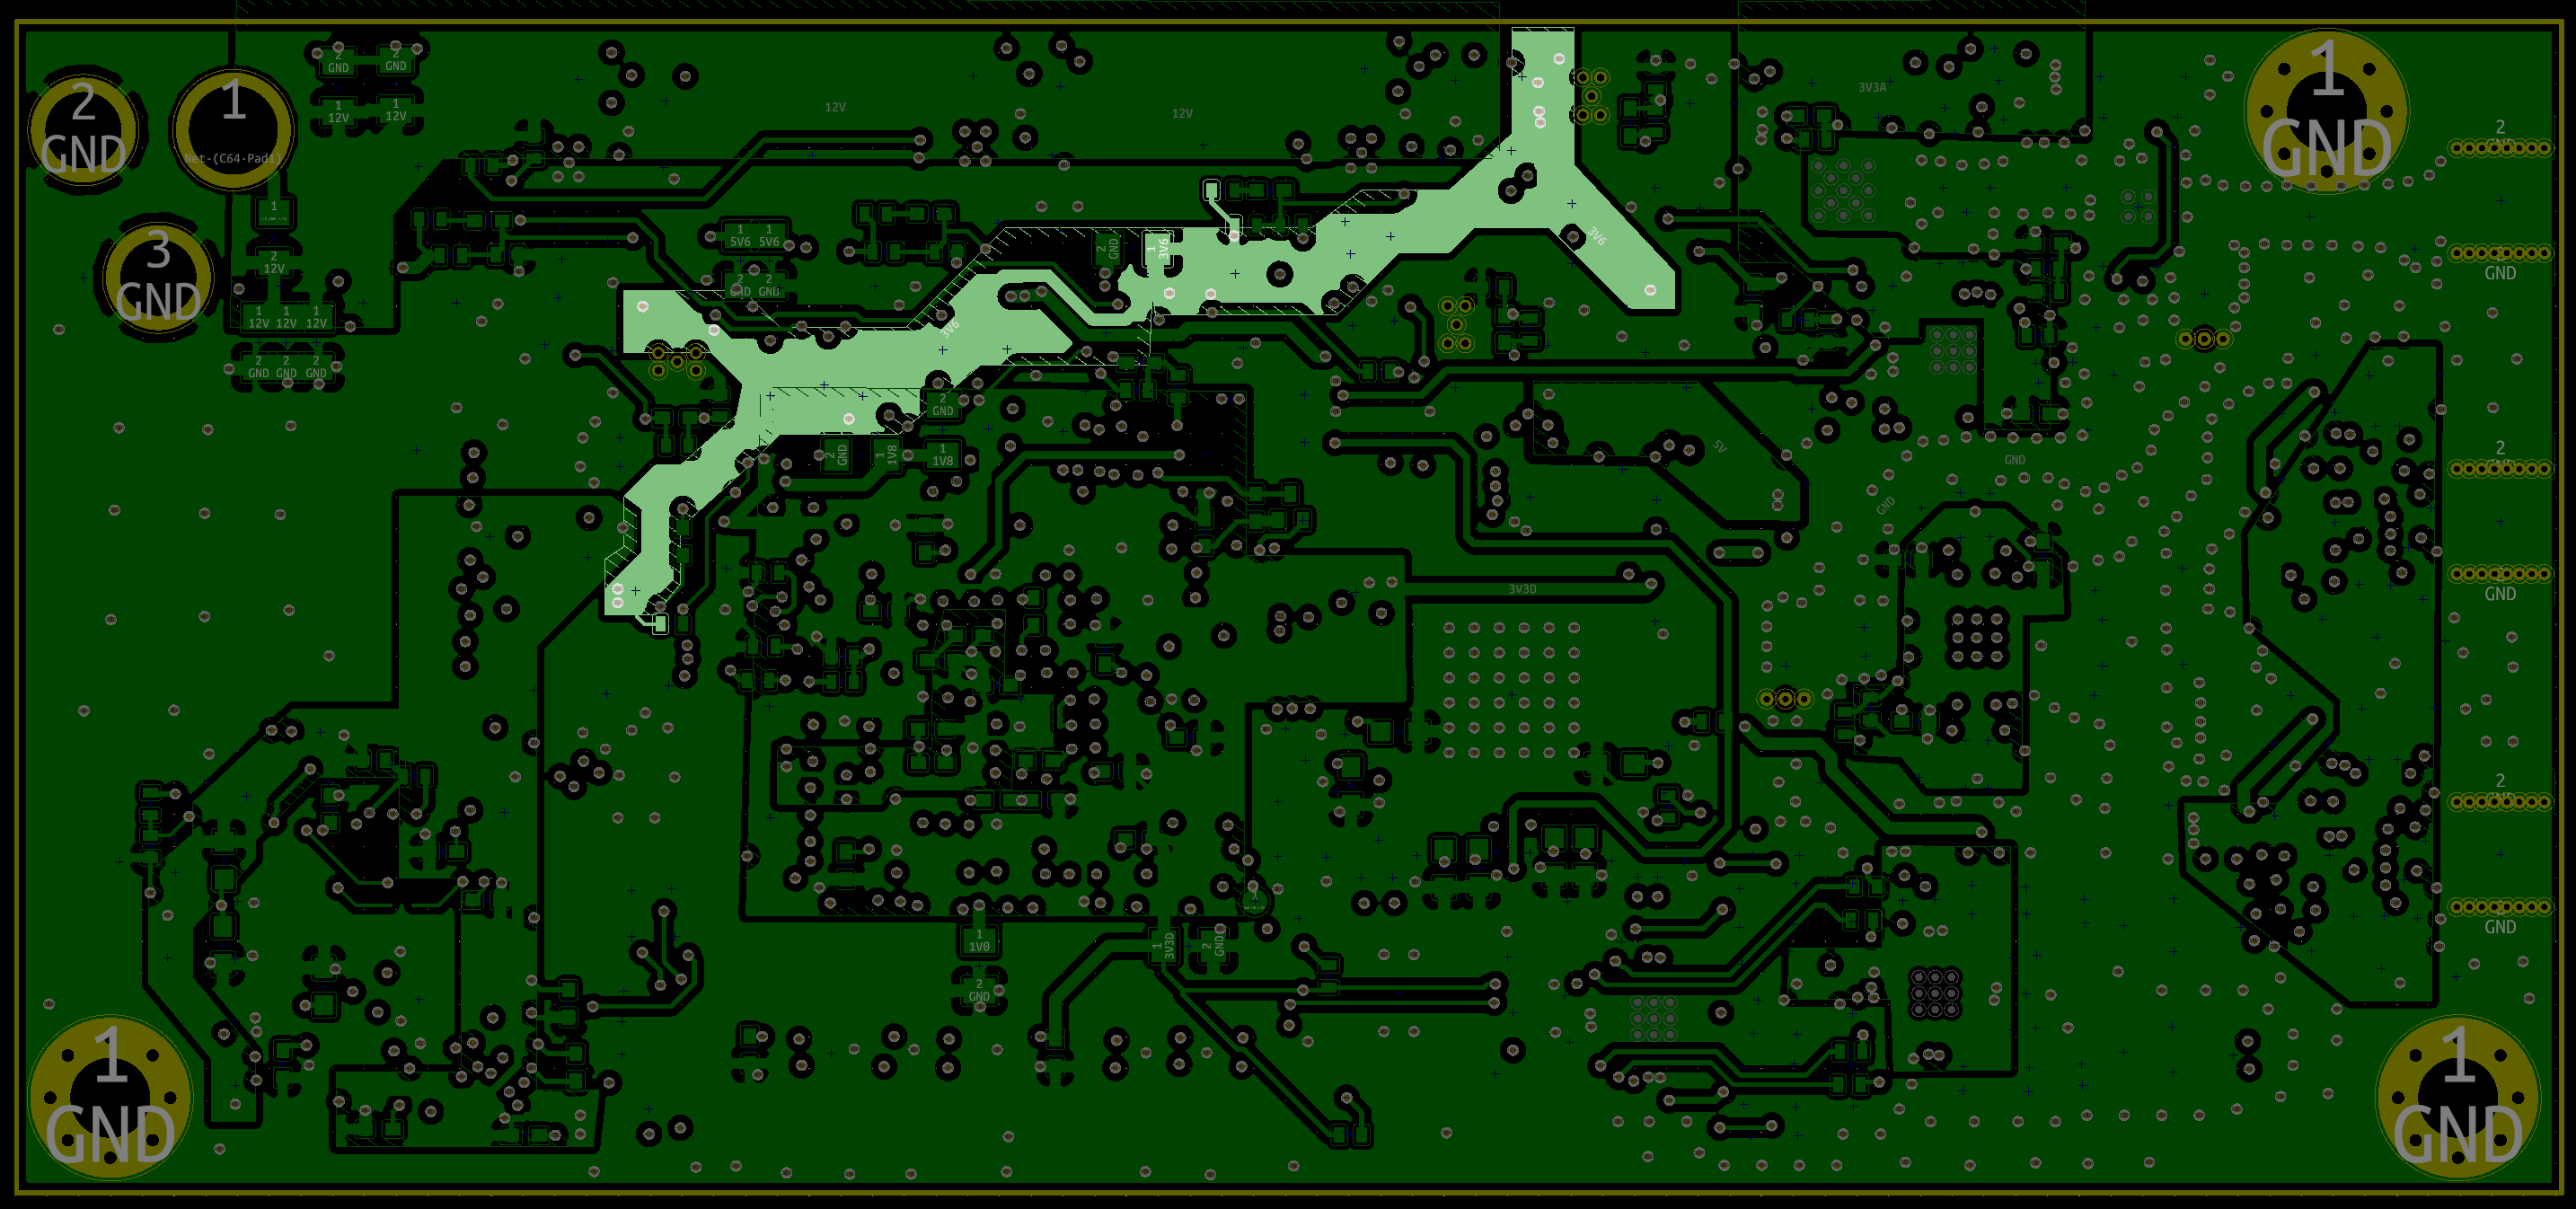
\includegraphics[width=\textwidth]{data/fmcw-layer4-3v6.png}
        \caption{There is a 3.6V power plane that is the output of one of the buck converter and is
          use as the input to several linear regulators that output 1.8V 3.0V and 3.3V.}
        \label{fig:fmcw-layer4-3v6}
\end{figure}

\begin{figure}[h]
        \centering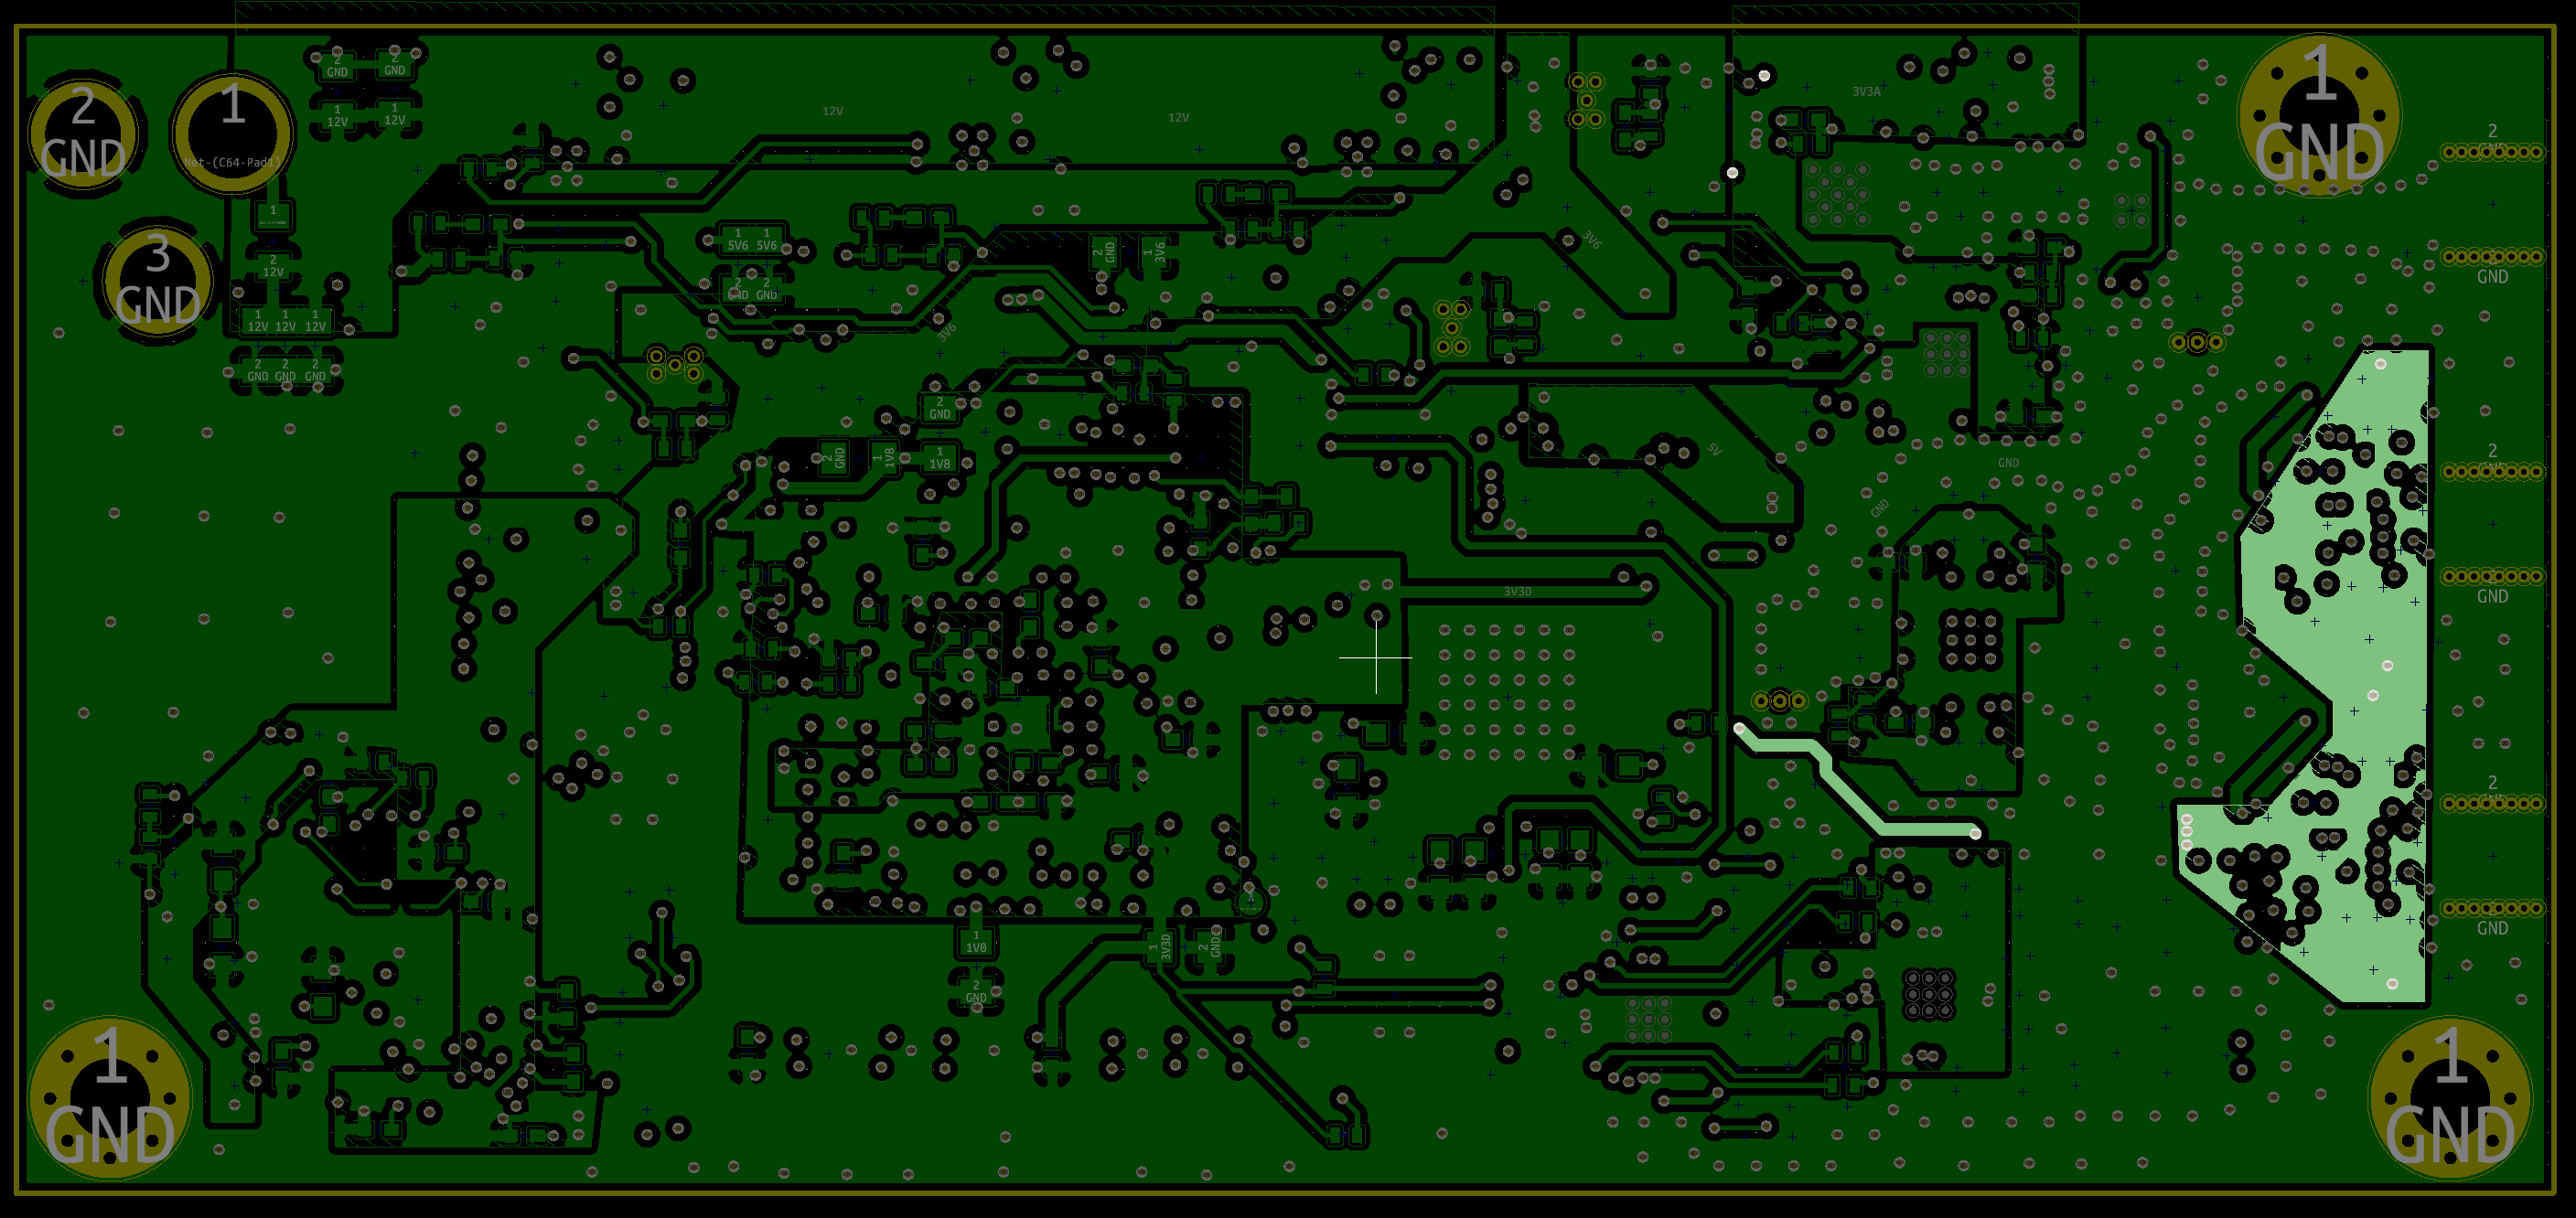
\includegraphics[width=\textwidth]{data/fmcw-layer4-3v0.png}
        \caption{A 3V power plane is used to power components near the right side of the boar (the
          righside of the board is where signal transmission and reception occur that amplify
          receive signals so they can be mixed with the transmitted signal and fed into the ADC
          before FPGA processing Notably, the 3V power plane is located near the components but far
          from the linear regulator that outputs it.}
        \label{fig:fmcw-layer4-3v0}
\end{figure}

\begin{figure}[h]
        \centering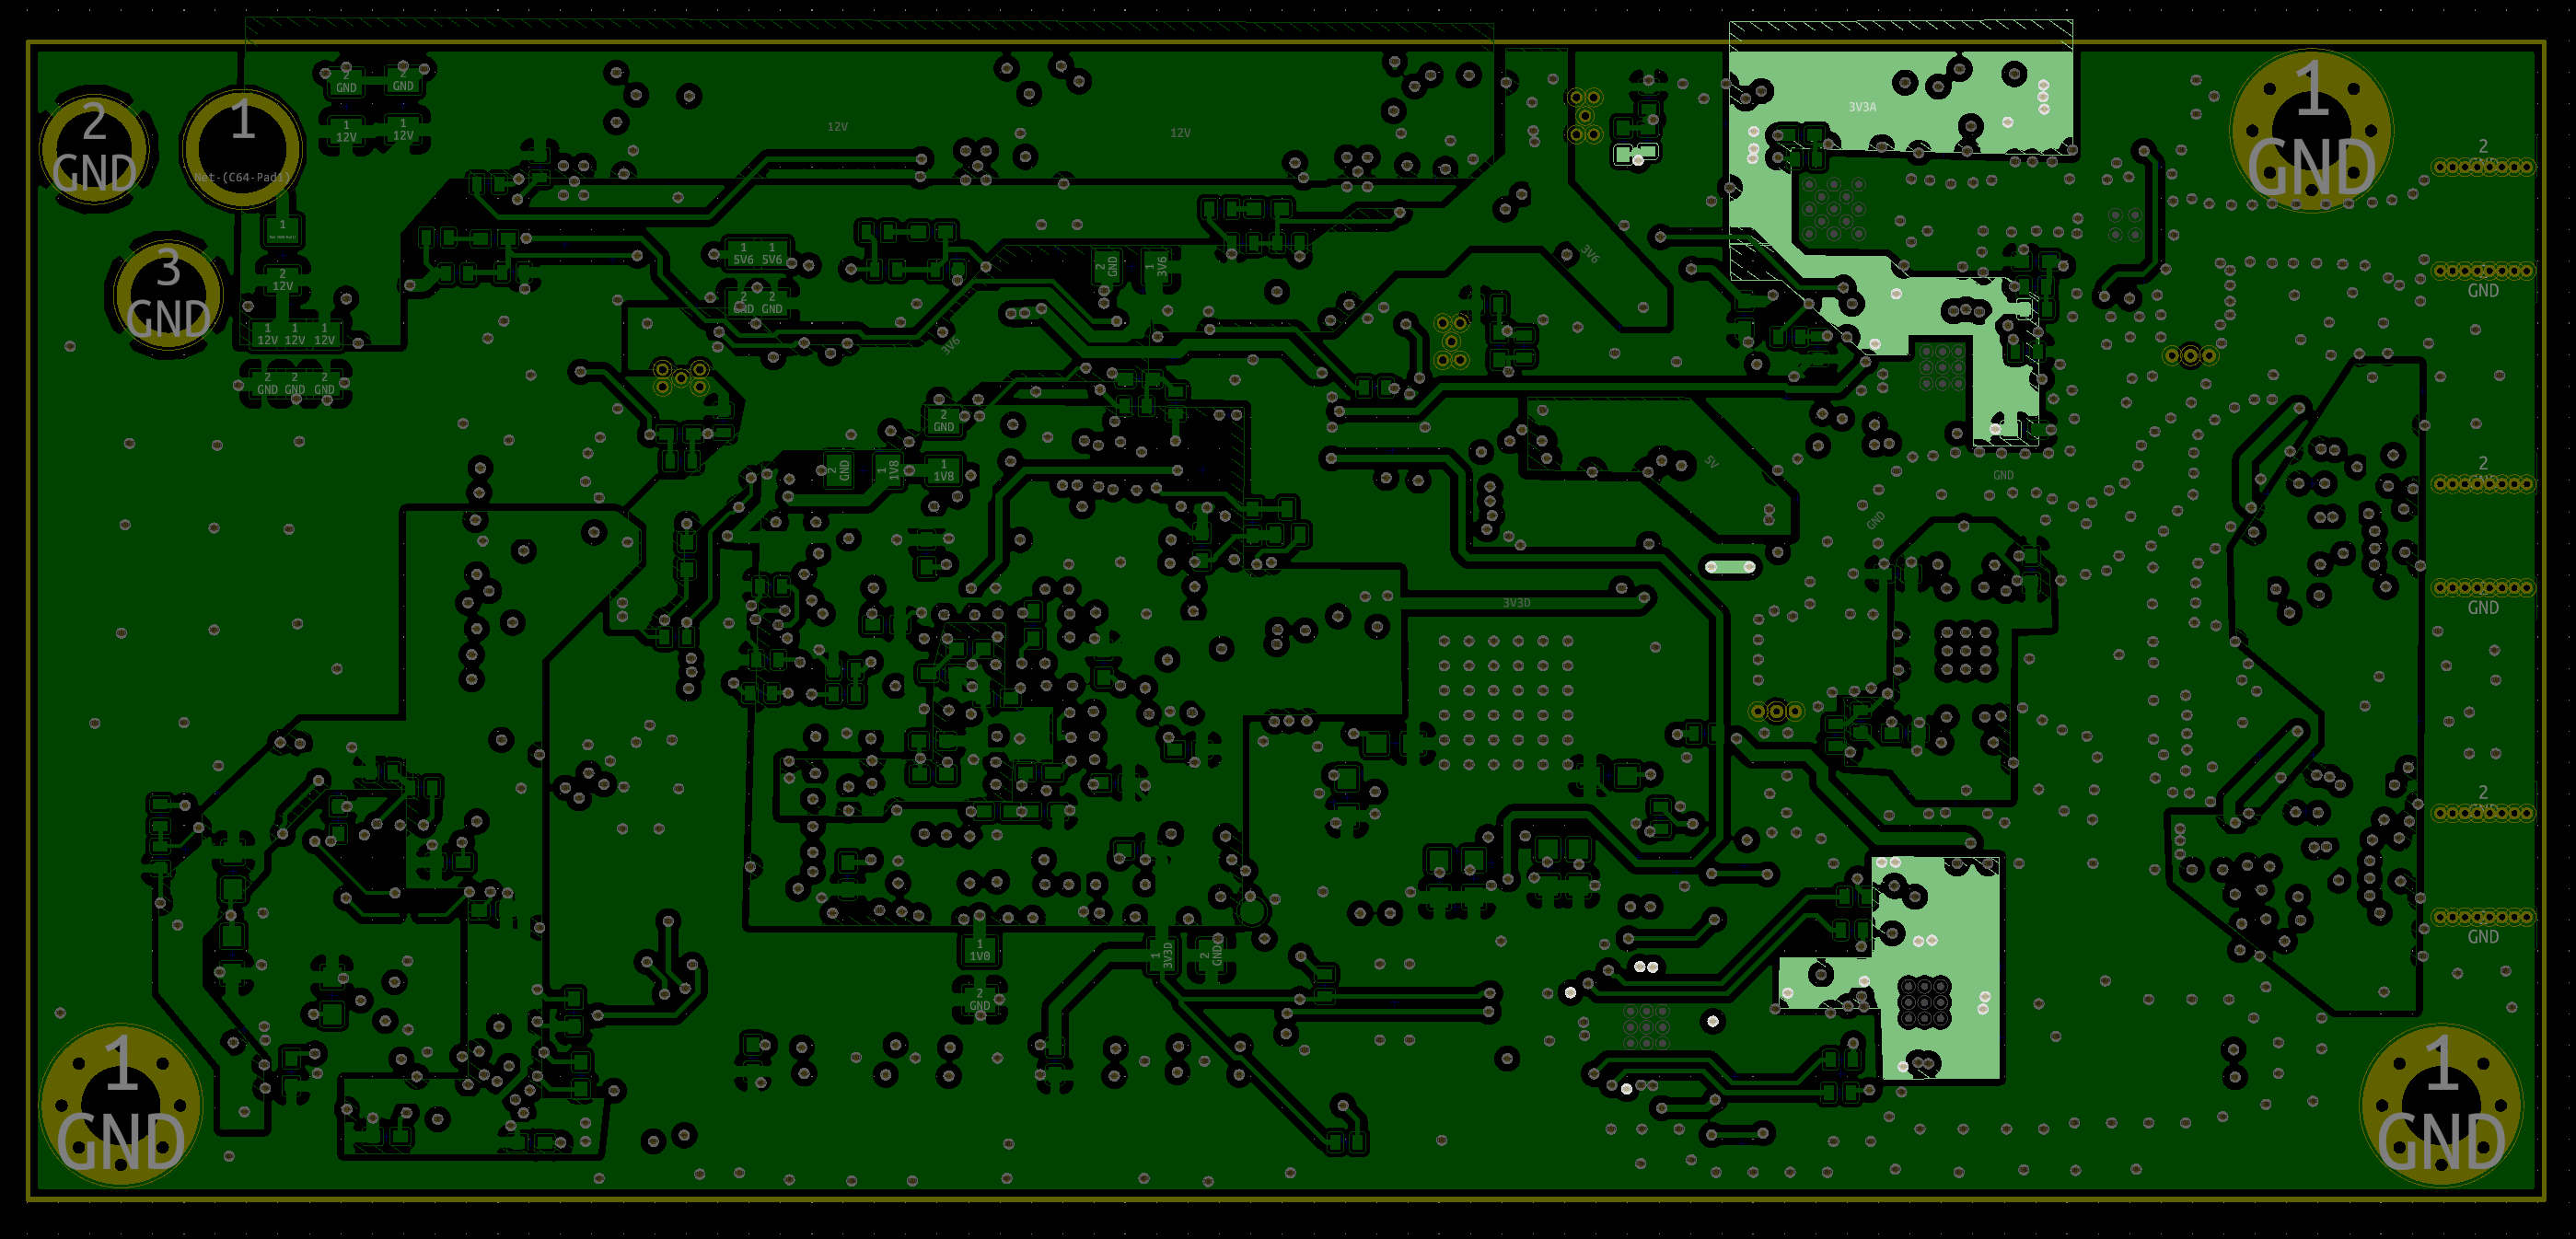
\includegraphics[width=\textwidth ]{data/fmcw-layer4-3v3a.png}
        \caption{A 3.3V power plane is used to power several components for signal transmission,
          such as a frequency synthesizer, and RF amplifier. These, along with all other reception
          and transmission circuitry, are located on the right side of the board.}
        \label{fig:fmcw-layer4-3v3a}
\end{figure}

\begin{figure}[h]
        \centering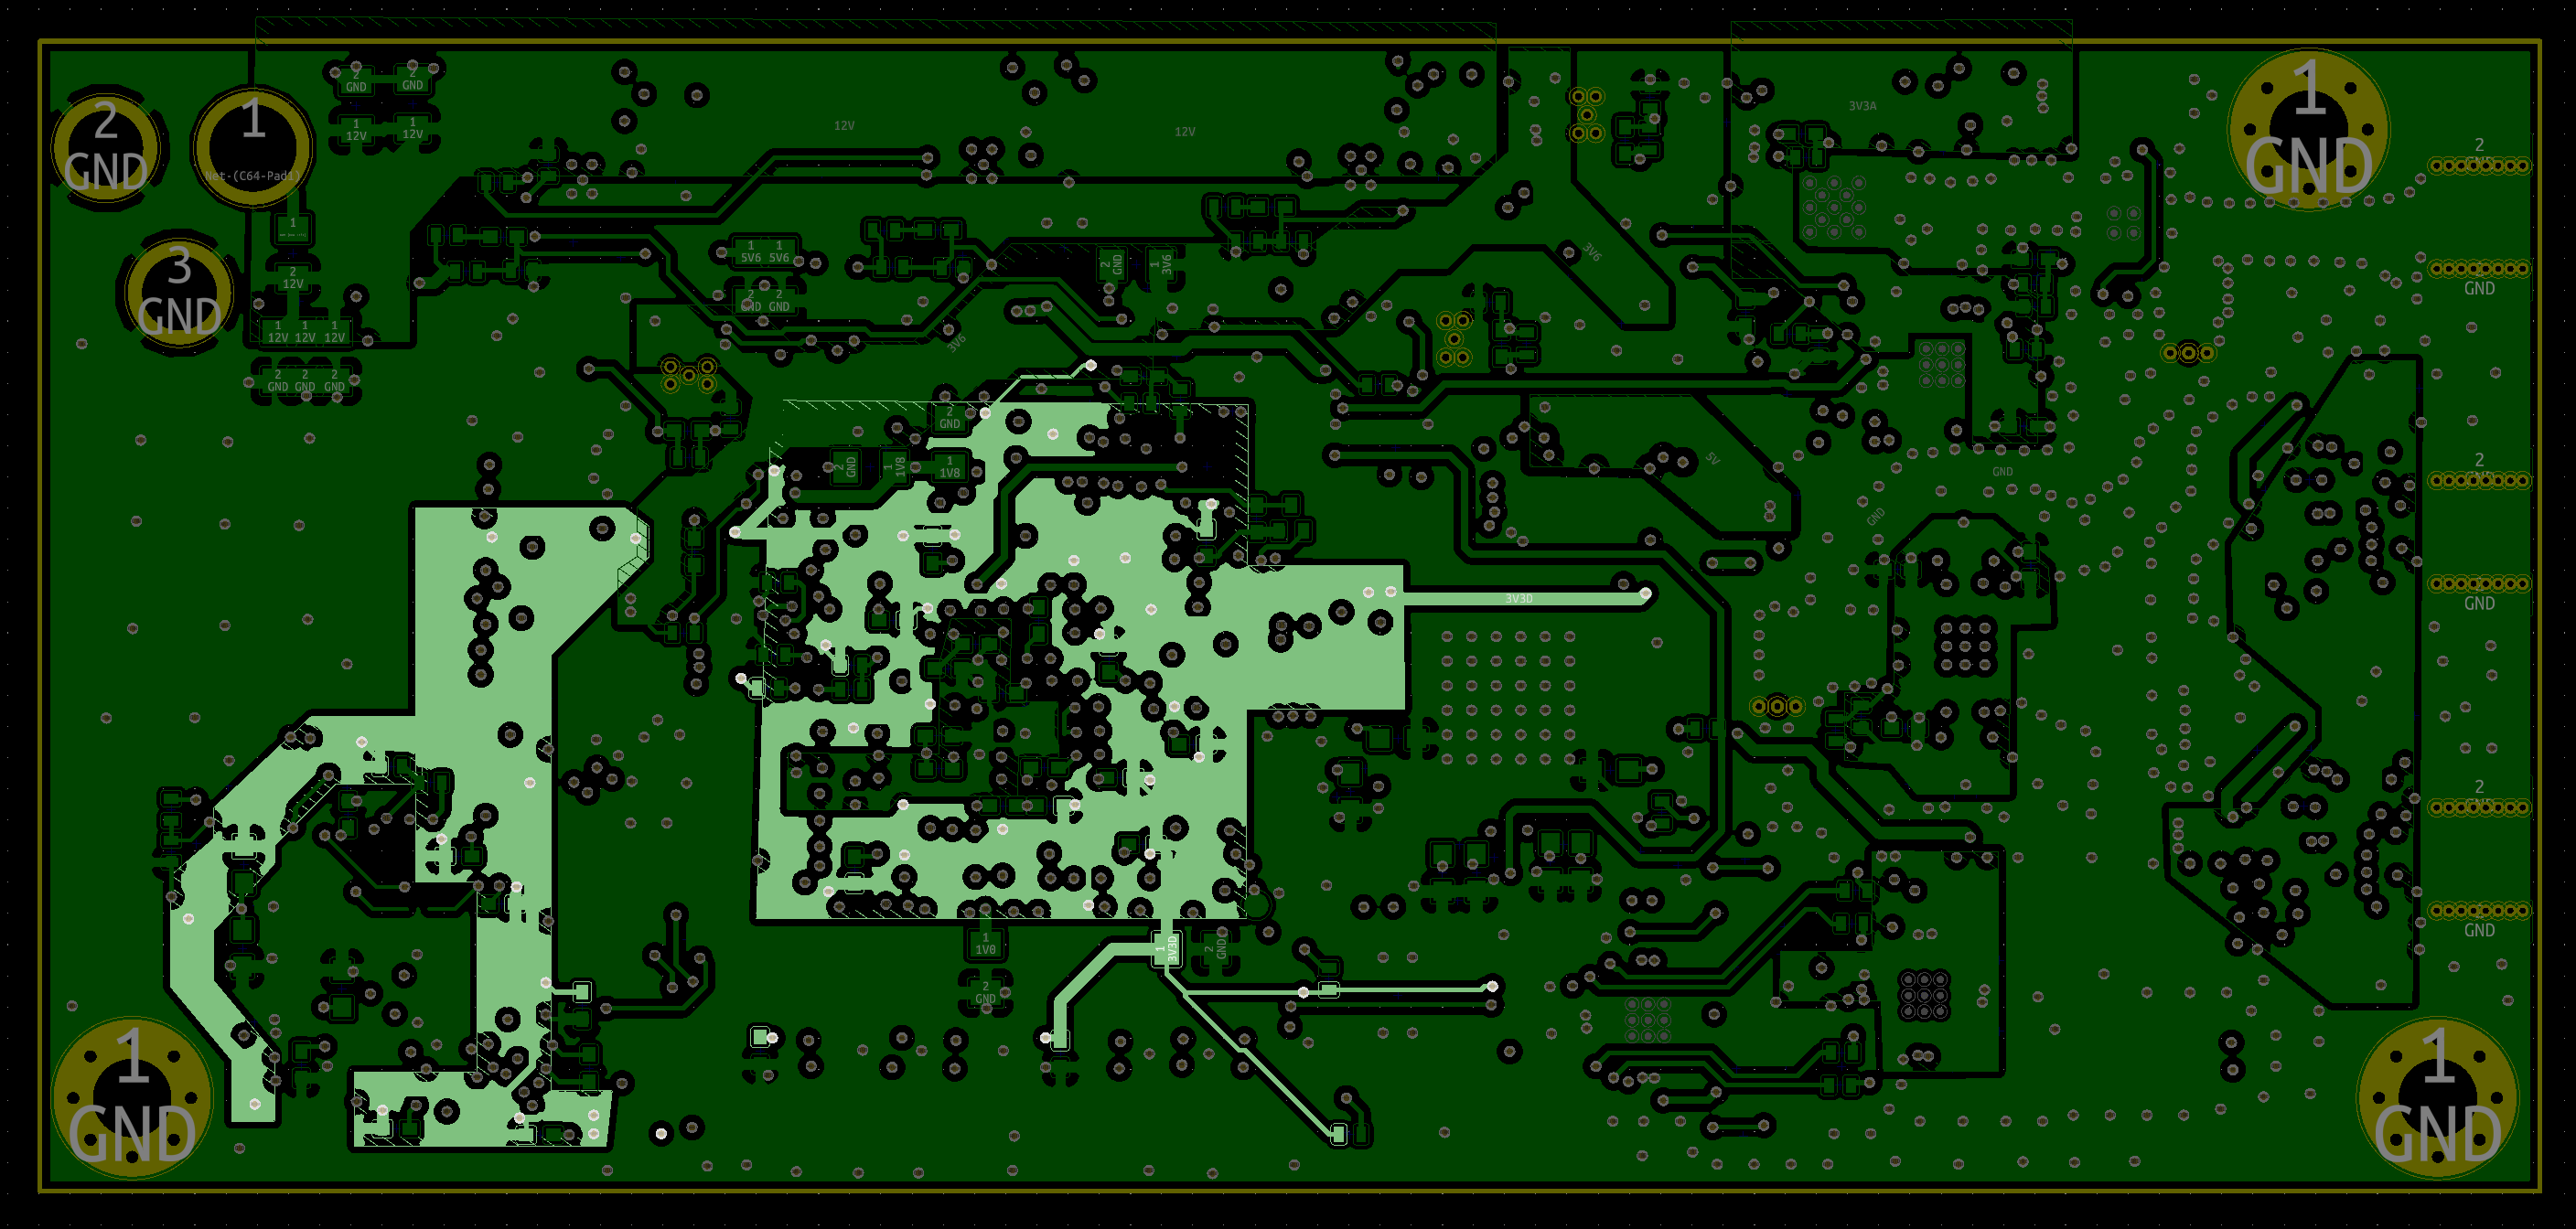
\includegraphics[width=\textwidth]{data/fmcw-layer4-3v3d.png}
        \caption{Another 3.3V power plane is used as one of the power inputs to the FPGA as well as
          to a USB-to-UART device (a configuration bit stream is sent from a host computer through a
          USB cable to the PCB where this device converts it into the proper UART format to be
          transmitted to the FPGA) and an ADC (the ADC converts the mixed transmitted-received
          signals to digital and thensends them to the FPGA for processing).}
        \label{fig:fmcw-layer4-3v3d}
\end{figure}

\begin{figure}[h]
        \centering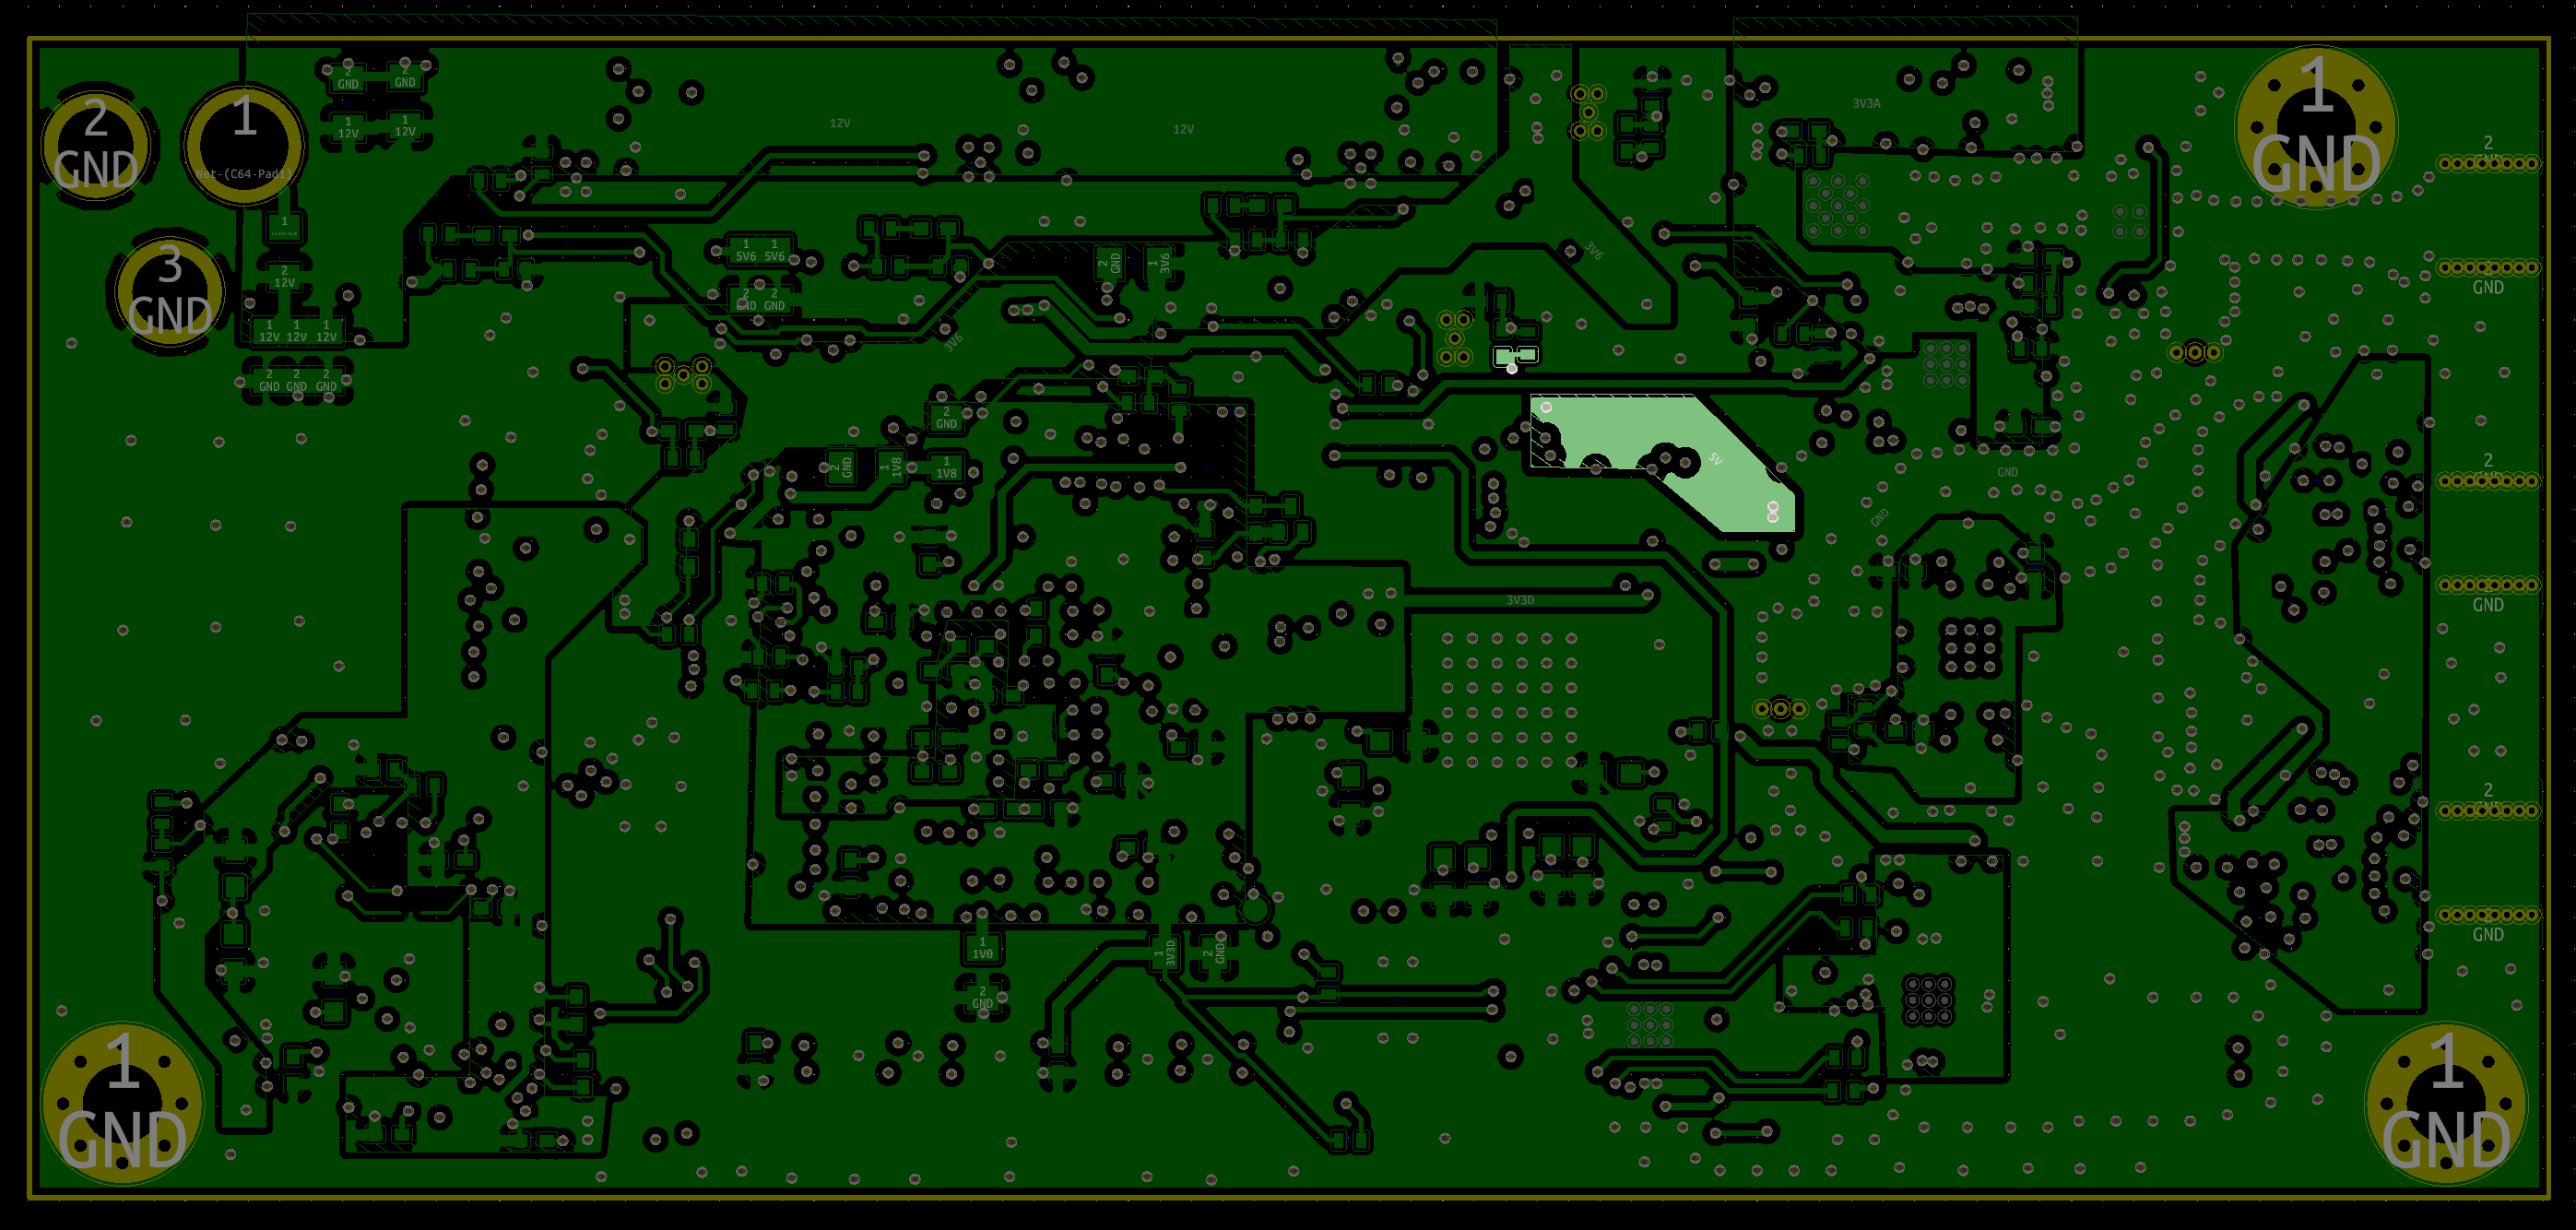
\includegraphics[width=\textwidth]{data/fmcw-layer4-5v.png}
        \caption{A 5V power plane powers one of the inputs to the frequency synthesizer for
          transmission.}
        \label{fig:fmcw-layer4-5v}
\end{figure}

\begin{figure}[h]
        \centering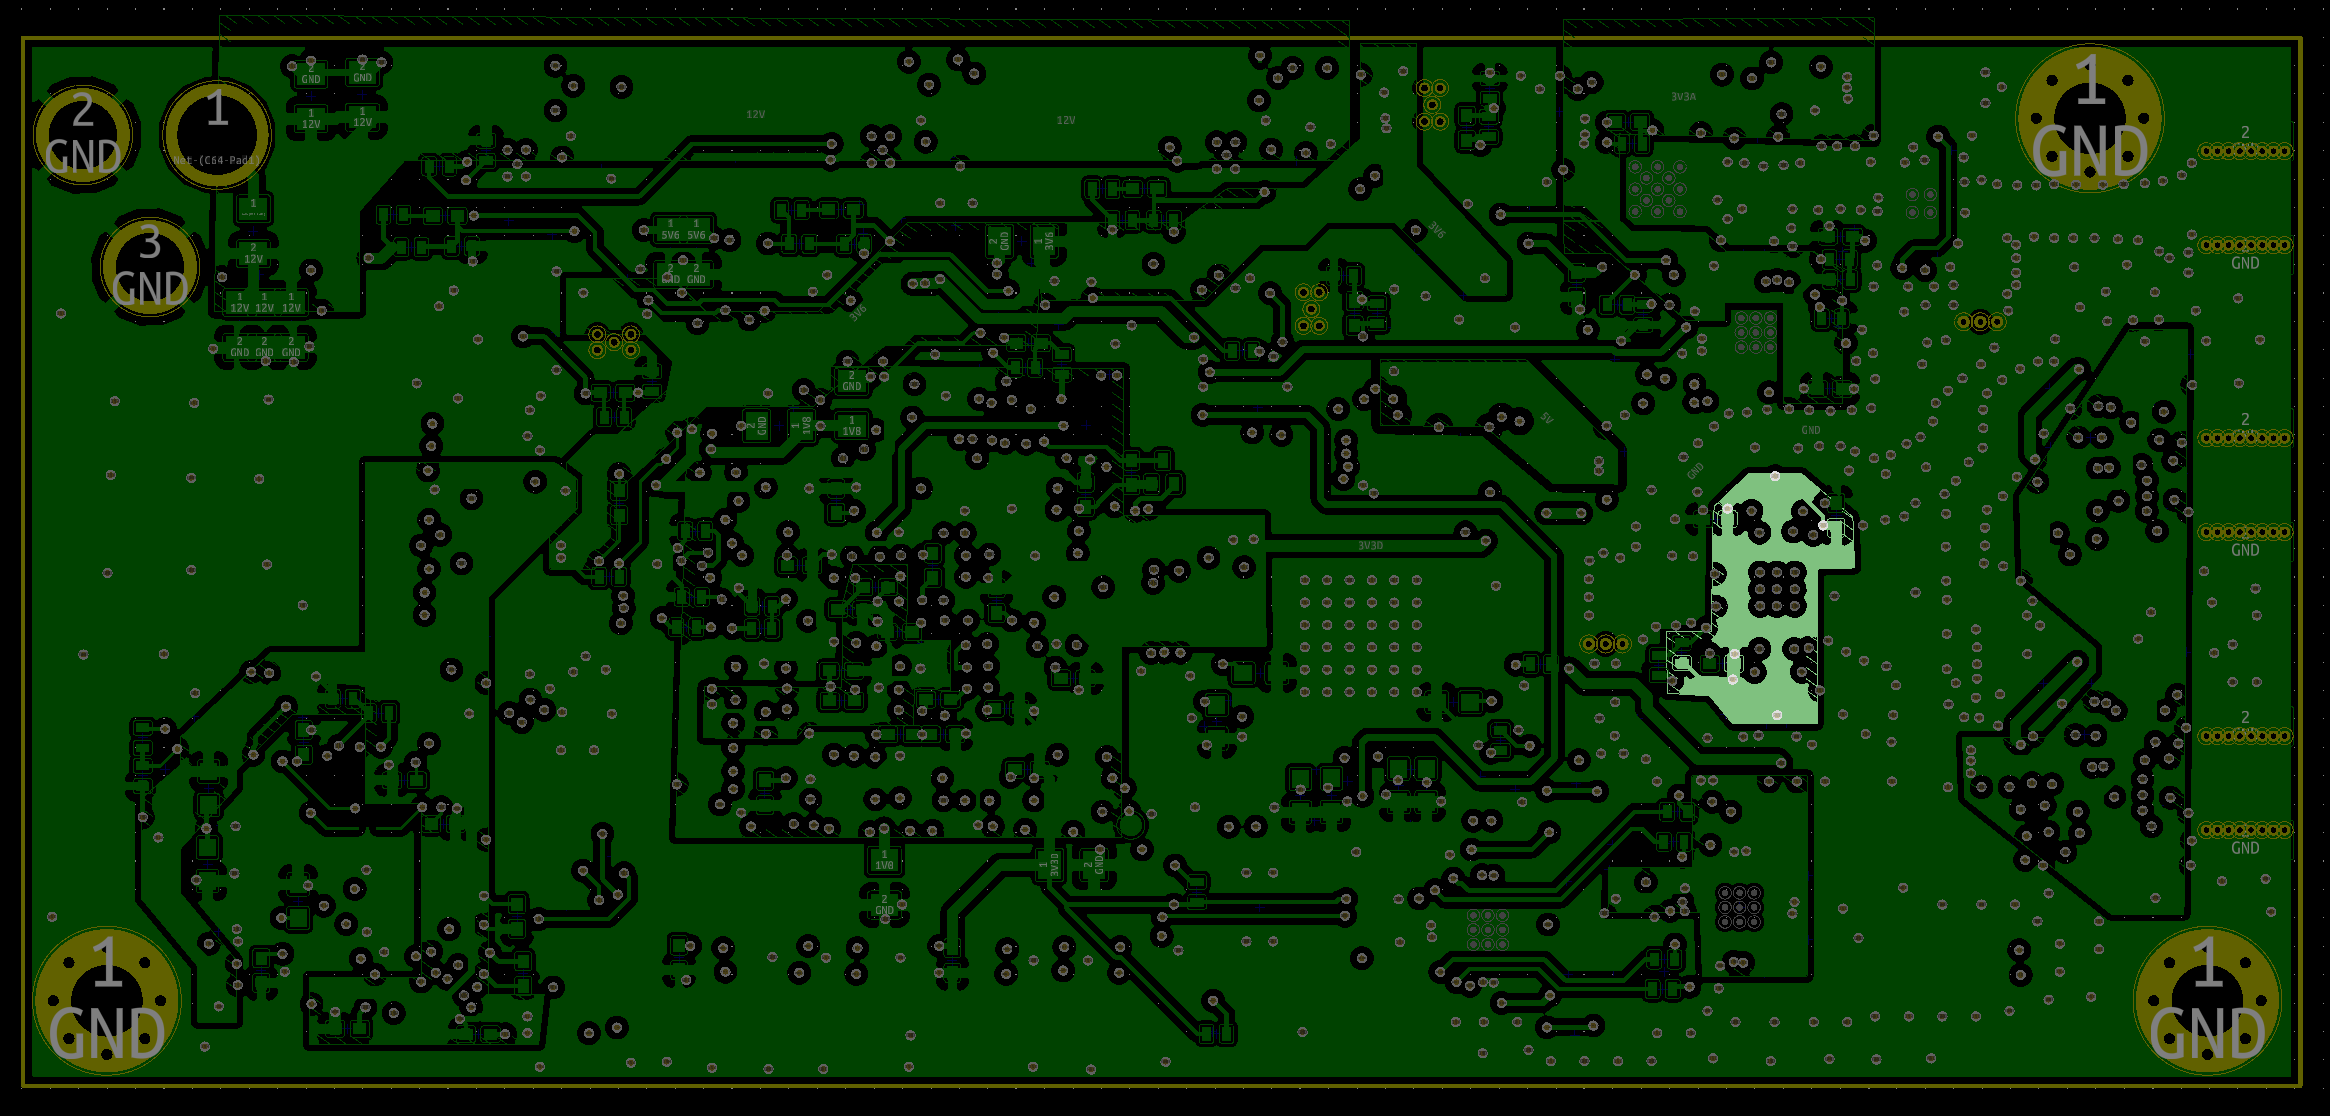
\includegraphics[width=\textwidth]{data/fmcw-layer4-5vf.png}
        \caption{Another 5V power plane is used for to power devices after going through a ferrite
          bead.}
        \label{fig:fmcw-layer4-5vf}
\end{figure}

\section{Component Layout Considerations}

\subsection{Power Input}
\label{sec:power-input-layout}

The barrel jack used has an inner diameter of 2.1mm and an outer diameter of 5.5mm and should output
12V. Since barrel jack dimensions and voltage output vary widely, special attention should be given
to make sure the actual hook up matches these specifications.

The pi filter should be placed as close to the barrel jack connection as possible so as to minimize
crosstalk noise with the rest of the board.

All components should be placed sufficiently close to the TPS5420D buck converter, except for the
trace between the voltage divider and VSNS which should be given a sufficiently wide berth from the
PH trace.

\subsection{LTC2292 ADC}

\begin{itemize}
\item The LTC2292 contains 4 positive voltage supply pins each requiring a 0.1$\mu$F bypass
        capacitor. One capacitor each should be placed directly adjacent to each of the 4 voltage
        supply pins.
\item The device contains 2 input pins for the voltage of the device where the output data is
        sent. These, similarly require a 0.1$\mu$F capacitor each. As before they should be placed
        next to their respective pins, not next to one another.
\item VCMA and VCMB each are connected to a 2.2$\mu$F capacitor to GND. They should be placed as
        close to the pins as possible.
\item REFHA and REFLA (and REFHB and REFLB) have a 0.1$\mu$F capacitor connected between them. These
        are the most critical capacitors connected to the ADC. They must be placed 1.5mm away at
        most, and preferably closer to the pins.
\end{itemize}

\subsection{RX1 / RX2}

\begin{itemize}
\item The 100pF capacitor used to bypass TRF37A73 should be place as close as possible to VCC.
\end{itemize}

\section{RF Impedance Matching}

\fixme{I don't think the text below is correct.}.

I'm keeping it for the value of knowing the trace widths used by the original design. However, the
idea that the trace widths are unimportant seems dubious. The PCB calculator built into KiCad should
be used for this. Additionally, it is probably worth looking at the following guides:
\href{https://www.maximintegrated.com/en/app-notes/index.mvp/id/5100#}{Maxim: General Layout
  Guidelines for RF and Mixed-Signal PCBs},
\href{https://hackaday.com/2016/03/23/michael-ossmann-makes-you-an-rf-design-hero/}{Hackaday:
  Michael Ossmann makes you an RF design hero},
\href{https://www.analog.com/media/en/training-seminars/design-handbooks/Basic-Linear-Design/Chapter12.pdf}{Analog}. I
would also look at \href{https://github.com/erichVK5/WilkinsonPowerDividerFootprintGenerator}{this
  tool} for creating a Wilkinson power divider. Also, the trace width for $50\si{\Omega}$ resistors
seems to have been more like 15mil.

Use \href{http://www.mantaro.com/resources/impedance-calculator.htm}{this Mantaro impedance
  calculator} to calculate trace widths. The proper width should be 11.98mil.

The right side of the board houses the RF circuitry (i.e. transmitter, receivers and SMA
connectors). The signals are carried to the antennas (a patch-fed horn for transmission and a patch
array for reception) via a $50\si{\Omega}$ coaxial cable. All RF inputs and outputs for components
should match this $50\si{\Omega}$ impedance. The original layout does not seem overly concerned with
the microstrip transmission line width between RF components. They are kept short and generally have
a trace width of about 0.3mm. However, many of them are not even remotely straight and this doesn't
seem to be an issue. Where possible the microstrips should be kept short, straight and with an
unbroken ground plane beneath them. That seems to be all that is necessary for impedance
matching. The patch antennas however will need to be appropriately hooked up in order to match the
$50\si{\Omega}$ impedance. This should be a relatively straightforward calculation. The setup Henrik
uses seems to be the most logical one. He uses a single patch-fed horn antenna for transmission and
a patch array for reception. The horn antenna is made of thin copper. More sophisticated horn
antennas require the ability to weld and probably modeling software (e.g. CST).

\chapter{Antennas}
\label{cha:antennas}

There are several promising places to start in learning how to do this. Obviously, the
\href{hforsten.com}{hforsten blog} is a good place. Contextual Electronics also has a
\href{https://www.youtube.com/watch?v=m0B-63Q-R_8}{youtube video} about building a PCB
antenna. Finally, \href{http://openems.de/index.php/Main_Page.html}{OpenEMS} is apparently a very
powerful tool for simulating and designing antennas (among other things RF). This is already
installed and can be scripted through Octave. Make sure to look at the tutorials.

One antenna is used for transmission and two are used for reception. It might be possible to achieve
the same effect with two overall antennas but the design would need to be significantly altered to
do so. The transmission antenna should have high gain and high directivity. This ensures sufficient
power for reception, longer range, and less side clutter (i.e. you don't want a wide field of
vision, you want this to be mostly directed in a single direction). We use two reception antennas
instead of one so that we can perform beamforming. Basically, we mix the signal picked up by each
reception antenna individually with the transmitted signal. Each of these mixed products tells us
the distance from the object. However, if the object is at a slight angle, the phase difference
between the two mixed products tells us the incident angle, so we can localize the distant object.

\href{https://assets.lairdtech.com/home/brandworld/files/ANT-DS-PA58\%201115.pdf}{This antenna}
looks like it would be good for
transmission. \href{https://shop.bizsyscon.com/rf-elements-sh-cc-5-30-symmetrical-horn-carrier-class-30-degree.html#horizontalTab1}{This
  RF Elements} antenna looks even better, but is more than I'm willing to pay (and its gain is
lower,
however). \href{https://smile.amazon.com/d/Sewing-Machines-Accessories/9-4dBi-Triple-Antenna-Terminator-RJX1749/B074PR4TW3/ref=sr_1_8?ie=UTF8&qid=1544680544&sr=8-8&keywords=patch+antenna}{The
  Triple Feed Patch Array Antenna} is a great deal for the price and is based off a clever
open-source design,
\href{http://www.maartenbaert.be/quadcopters/antennas/triple-feed-patch-array-antenna/}{here}. I'm
not sure if the gain will be quite enough, however. If you're confused about the operation of that
last one, look at the description for it on Antenna Test Lab. They provide excellent
information. I'm mostly struggling to find a good patch array antenna for reception. I may have to
just build this myself, but I'm worried about the quality using normal FR4.

\chapter{Links}
\label{cha:links}


\chapter{Full Schematic}
\label{cha:schematic}

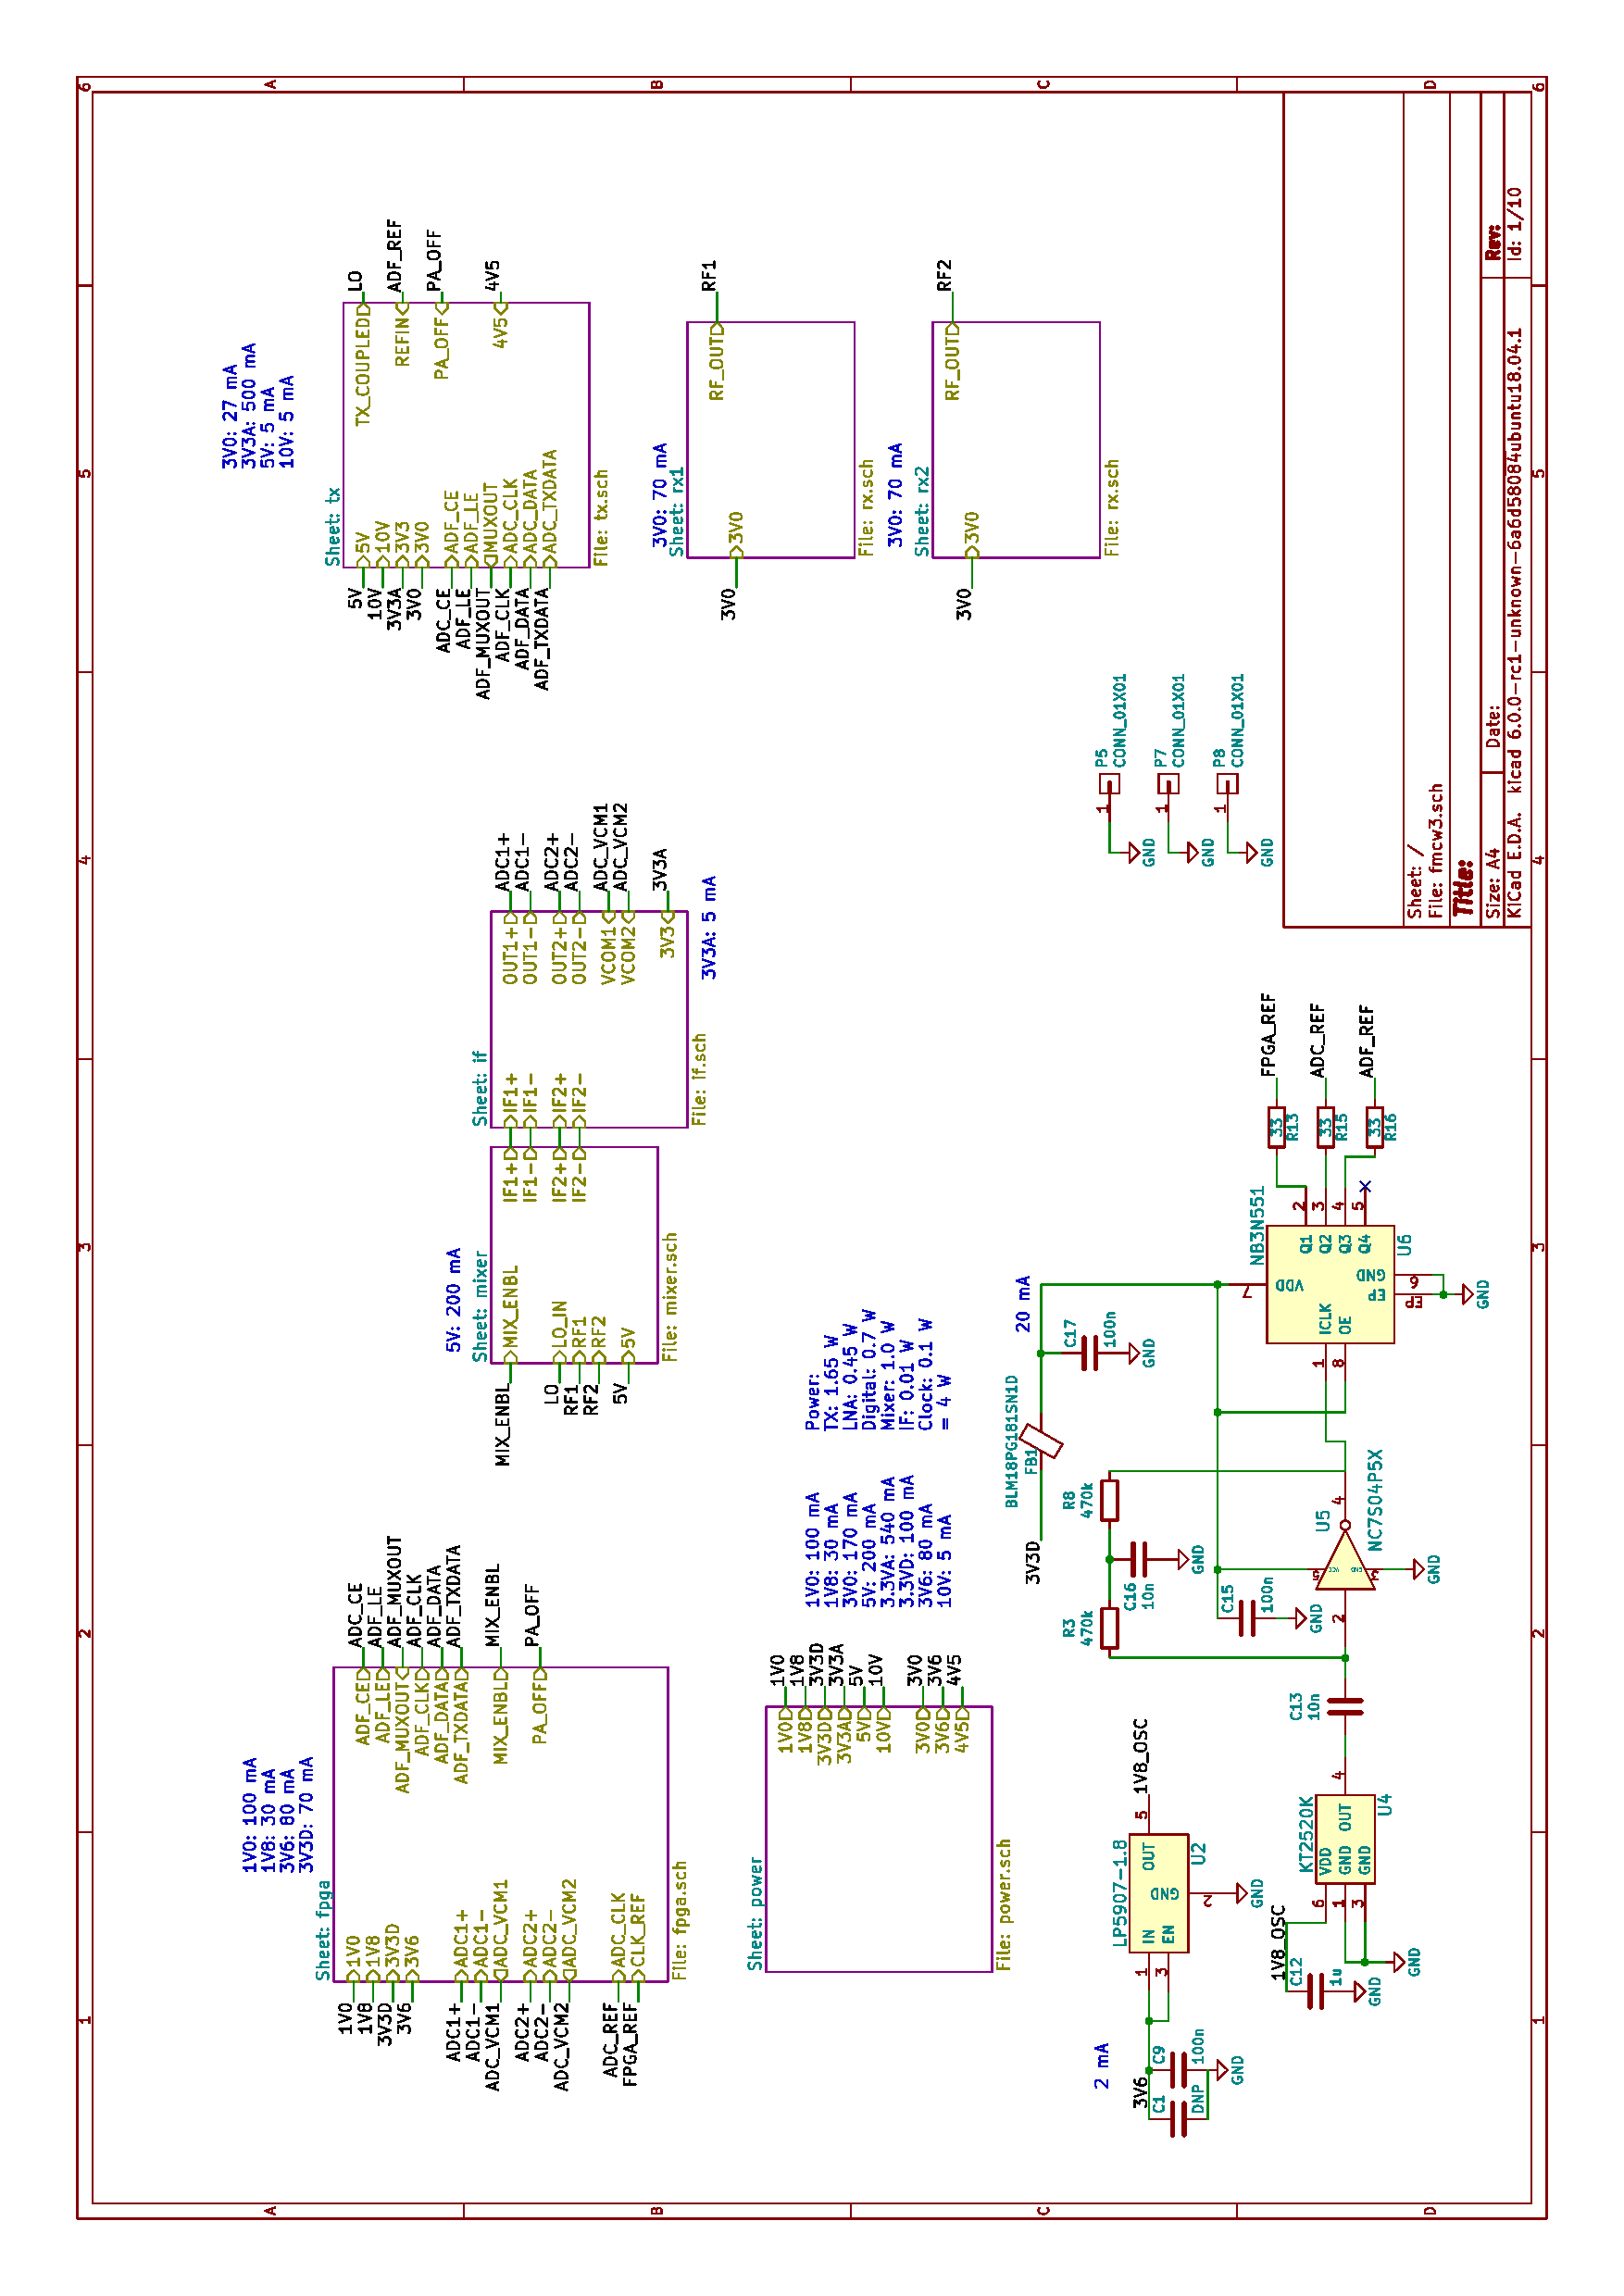
\includepdf[pages=-, link, linkname=schematic, landscape=true, angle=-90,
pagecommand={\refstepcounter{includepdfpage}\label{schematic.\theincludepdfpage}}]{data/fmcw-schematic.pdf}


\end{document}
%%% Local Variables:
%%% mode: latex
%%% TeX-master: t
%%% End:
